%
% File acl2014.tex
%
% Contact: koller@ling.uni-potsdam.de, yusuke@nii.ac.jp
%%
%% Based on the style files for ACL-2013, which were, in turn,
%% Based on the style files for ACL-2012, which were, in turn,
%% based on the style files for ACL-2011, which were, in turn, 
%% based on the style files for ACL-2010, which were, in turn, 
%% based on the style files for ACL-IJCNLP-2009, which were, in turn,
%% based on the style files for EACL-2009 and IJCNLP-2008...
%% Based on the style files for EACL 2006 by 
%%e.agirre@ehu.es or Sergi.Balari@uab.es
%% and that of ACL 08 by Joakim Nivre and Noah Smith

\documentclass[11pt]{article}
\usepackage{acl2014}
\usepackage{times}
\usepackage{url}
\usepackage{latexsym}
\usepackage{amsmath}
\usepackage{xspace}
\usepackage{enumitem}
\usepackage[small]{caption}
\usepackage{longtable}

\usepackage[usenames,dvipsnames,svgnames,table]{xcolor}
\usepackage{soul}

\usepackage{algorithm}
\usepackage[noend]{algpseudocode}
\usepackage{graphicx}
\usepackage{caption}
\usepackage{subcaption}

\usepackage{tikz-dependency}

\newcommand{\eqnref}[1]{\eqref{eqn:#1}}

\usepackage[usenames,dvipsnames,svgnames,table]{xcolor}  % allows better color names
\usepackage{todonotes}   % insert [disable] to disable all notes
% Note that these macros accept optional arguments such as 
% [size=\small,bordercolor=red].
\newcommand{\Note}[4][]{\todo[author=#2,color=#3,fancyline,#1]{#4}}
\newcommand{\noteJH}[2][]{\Note[#1]{JH}{blue!40}{#2}}
\newcommand{\noteJE}[2][]{\Note[#1]{JE}{green!40}{#2}}   
\newcommand{\notewho}[3][]{\Note[#1]{#2}{orange!40}{#3}}  % extra arg with miscellaneous author
\newcommand{\NoteJH}[2][]{\noteJH[inline,#1]{#2}}
\newcommand{\NoteJE}[2][]{\noteJE[inline,#1]{#2}}
\newcommand{\Notewho}[3][]{\notewho[inline,#1]{#2}{#3}}  % extra arg with miscellaneous author

% \newcommand{\root}{\texttt{\$}}


\title{Deriving Multi-Headed Projective Dependency Parses \\ from Link Grammar Parses}
% Oriented link grammar: Creating a multi-headed dependency corpus.

% \author{Juneki Hong and Jason Eisner\\
%   Department of Computer Science \\
%   Johns Hopkins University \\
%   Baltimore, MD 21218, USA \\ 
%   {\tt \{juneki,jason\}@cs.jhu.edu} \\
% }

\date{}

\setlength\titlebox{3cm}    % Expanding the titlebox

\begin{document}
\maketitle

\begin{abstract}
Under multi-headed dependency grammar, a parse is a directed acyclic graph rather than a tree.  Such formalisms can be more syntactically and semantically expressive.  However, 
it is hard to train, test, or improve multi-headed parsers because few multi-headed corpora exist, particularly for the projective case.
% OLD
% investigate the benefit of such parsers or to work on making them faster or more accurate.  
To help fill this gap, we observe that link grammar already produces {\em undirected} projective graphs.  
% OLD
% ... produces parses that are similar to multi-headed projective dependency parses, except that the links are undirected. 
We use Integer Linear Programming to assign consistent directions to the labeled links in a corpus of several thousand parses produced by the Link Grammar Parser, which has broad-coverage hand-written grammars of English as well as Russian and other languages.  We find that such directions can indeed be consistently assigned in a way that yields valid multi-headed dependency parses. The resulting parses in English appear reasonably linguistically plausible, though differing in style from CoNLL-style parses of the same sentences; we discuss the differences.  
\end{abstract}

\section{Multi-Headed Dependency Parsing}

Dependency parsing maps a sentence to a directed graph whose vertices are the words $1, 2, \ldots, n$ of the sentence along with a distinguished ``root'' vertex 0.  A labeled directed edge $u \stackrel{L}{\rightarrow} v$ or $v \stackrel{L}{\leftarrow} u$ indicates that the ``child'' $v$ is some kind of argument or modifier of its ``parent'' $u$.  The edge label $L$ indicates the specific syntactic or semantic relationship between the two words.  

In the special case $u=0$, the edge designates $v$ as playing some special top-level role in the sentence, e.g., as the main verb.  We disallow $v=0$.

As recently discussed by \newcite{gomezrodriguez-nivre-2013}, one might impose various requirements on the parse graph:
\begin{itemize}[noitemsep]
\item {\sc Single-Head}: each word has $\leq 1$ parent
\item {\sc Acyclic}: there are no directed cycles
\item {\sc Connected}: each pair of words has a undirected path between them
\item {\sc Reachable}: each word can be reached from 0 by a directed path ($\Rightarrow$ {\sc Connected})
\item {\sc Planar}: edges may not ``cross''\footnote{That is, if there are edges between $i,j$ and between $u,v$, where $i < u < j$, then {\sc Planar} requires $i \leq v \leq j$.}
\end{itemize}
It is common to impose all of these requirements at once, leading to a {\em projective dependency parser} that produces projective trees rooted at 0.\footnote{{\sc Projective} basically means {\sc Planar} + {\sc Reachable}.  Note: It does not prevent 0 from having multiple children.}  However, parsing algorithms can be devised that relax any or all of the requirements \cite{gomezrodriguez-nivre-2013}.  

In this paper, we are interested in relaxing the {\sc Single-Head} requirement while preserving all the others.  This means that the parse can have more than $n$ edges, allowing it to express more relationships between words.  In English, for example, here are some constructions that seem to call for a multi-headed analysis.  
\begin{description}
\item[control] In {\em ``Jill likes to skip,''} the word {\em Jill} is the subject of two verbs.  In {\em ``Jill persuaded Jack to skip,''} {\em Jack} is the object of one verb and the subject of another.  Without recognizing this, our parser would miss the syntactic invariants that {\em skip} always has a subject and {\em persuaded} always has an object.  It would also be unable to exploit the selectional preferences of both verbs to help disambiguate the parse.  This is why we prefer to make the parser aware of multi-headedness, rather than using a single-headed parser and then extracting the additional semantic roles from its output.
\item[relativization] In {\em ``The boy that Jill skipped with fell down,''} the word {\em boy} is the object of {\em with} as well as the subject of {\em fell}.  Without recognizing this, we would miss the syntactic invariant that {\em with} always has an object.  
\item[conjunction] In {\em ``Jack and Jill went up the hill,''} {\em Jack} and {\em Jill} serve as the two arguments to {\em and}, but they are also semantically subjects of {\em went}.  Without recognizing this, we would have no (local) reason for expecting the arguments of {\em and} to be nouns.
\end{description}

In linguistics, it is common to analyze some of these structures using trees with ``empty categories.''  The subject of {\em skip} is taken to be a silent morpheme {\em PRO}:
{\em ``Jill$_i$ likes PRO$_i$ to skip.''}  However, this is no longer a tree if one considers the implicit undirected edge between {\em Jill} and {\em PRO} (denoted by their shared index $i$).  Our simpler representation contracts this coreference edge, eliminating {\em PRO} and creating a {\em Jill} $\leftarrow$ {\em skip} link.  

\section{Link Grammars}

A few past NLP papers have explored multi-headed dependency parsing \cite{buchkromann-2006,mcdonald-pereira-2006,sagae-tsujii-2008,gomezrodriguez-nivre-2013}.  Unfortunately, there seem to be no annotated corpora in this form other than the Danish Dependency Treebank \cite{kromann-2003}; researchers have sometimes converted corpora from other formats such as HPSG.  

% ADDRESSED BY ABOVE?
% \NoteJE{We should acknowledge that another option would be to post-process either CoNLL parses or our link parses to automatically add more multi-heading, e.g., to handle control phenomena ("John wants to skip" or "Jane ran for office in order to change the tax laws" should have John/Jane be the subject of two verbs).  However, that requires per-language}

All of these options result in non-projective parses, so the parsers must use non-projective or pseudo-projective algorithms.

It seems at first that no one has worked out annotation conventions for {\em projective} multi-headed dependency parsing.  However, this is not quite true.  Link Grammar \cite{SleatorTemperly91} is a grammar-based formalism for projective dependency parsing with {\em undirected} links.  It produces undirected connected planar graphs.  Annotation conventions are implicit in the detailed lexicon for the Link Grammar Parser,\noteJE{check caps}%
\footnote{\url{http://www.abisource.com/projects/link-grammar/dict/introduction.html}.  The 122 link types in the English lexicon are documented at \url{http://www.abisource.com/projects/link-grammar/dict/summarize-links.html}.} 
which specifies for every word a constraint on the {\em sequence} of labeled leftward and rightward edges attached to it.  As remarked by \newcite{eisner-2000-iwptbook}, this is analogous to dependency grammar's use of head automata to constrain a word's sequence of left and right children.  For example, in {\em ``The boy that Jill skipped with fell down,''} the word {\em with} uses a lexical entry that requires it to link to a governing verb to the left, an extracted object farther to the left, and nothing to the right.  Each entry has a hand-assigned cost in \{0,1,2\} and the parser finds the parse of minimum total cost.
% Information about cost is in this message from Linas Vepstas on 2014-02-01: 
%   https://groups.google.com/d/msg/link-grammar/eeJw1Ofgc9U/diqPYSwuFfoJ

Given a link grammar parse, it would be straightforward to convert it to an acyclic dependency parse by orienting all edges rightward.  However, the result may violate the {\sc Reachable} constraint.  Instead we could orient all edges by depth-first search from the root node, which yields a DAG satisfying all our constraints.  However, this might result in inconsistent annotation conventions, with some \texttt{S}-labeled links pointing from subject to verb and others from verb to subject.  

We supposed that the link grammar lexicon designers actually had a consistent direction in mind for each edge type.  We would expect verbs to point to their subject arguments in dependency grammar, and so we surmise that all \texttt{S} links are intended to point leftward (from verb to subject: {\em ``Jack $\stackrel{\texttt{S}}{\leftarrow}$ is falling''}).  The link grammar designers take care to use a distinct \texttt{SI} label in cases of subject-verb inversion, and we surmise that \texttt{SI} links are intended to point rightward (again from verb to subject: {\em ``Is $\stackrel{\texttt{SI}}{\rightarrow}$ Jack falling?''}).

Our goal in this paper is to recover these implicit directions by global optimization.  We seek a fixed mapping from labels to directions such that link grammar parses become directed dependency parses that satisfy all of our constraints.

Our first thought was to seek a direction mapping such that no parsed word sequence allowed by the link grammar lexicon could possibly violate our constraints after directions were imposed.  This is a well-defined constraint programming problem.  For example, to prevent cyclicity, we would require (roughly speaking) that no word type in the lexicon could follow a sequence of directed rightward links through other word types and then a leftward link back to itself.  

However, working directly with the link grammar lexicon format is somewhat tricky.  We also feared that there would not be a perfect solution---for example, because of errors in the lexicon, or linguistically unnatural word sequences not anticipated by the grammar designers.  In this case it would not be clear how to relax our constraints.

Thus, we chose to use a sample of {\em actual} sentences parsed by the link grammar, and to seek a direction mapping so that {\em these} parses would not violate our constraints after directions were imposed.  If no such mapping exists, then we are willing to orient a few edge tokens in the wrong direction to ensure that the parses are still well-formed---but we minimize the number of such violations.  In this way, the empirical distribution of sentences guides our assignment of directions.  The resulting directed corpus can be used for research on multi-headed dependency parsing.

% Link grammars are a grammatical system equivalent to context-free grammars that assign linking requirements to every given word. A link parser then tries to satisfy all of these requirements for every word of a sentence while still maintaining planarity. The resulting links describe the relationships between constituents in a parse. 

% The link grammar is based on a set of handwritten dictionaries. Instead of going through these dictionaries, we learned the grammar using an ILP. This approach also potentially allows us to analyze link grammar dictionaries other than English. \todo{explore other link grammar dictionaries} 

% \NoteJE{what statistics does it use?  what languages are available}

% Link parsing in contrast produces a multiheaded planar graph with undirected edges, where every edge has a label describing the relationship between two constituents in a parse. In this paper we explore whether these relationships include dependencies, and whether the multiheadedness of the link grammar offers additional dependency relationships not found in other corpora.

% Dependency parsing is the task of mapping a sentence to a projective (not always projective?) directed acyclic tree. Link parsing in contrast produces a multiheaded planar graph with undirected edges, where every edge has a label describing the relationship between two constituents in a parse. In this paper we explore whether these relationships include dependencies. To determine the directional dependencies within the link edge labels we will use integer linear programming, encoding the problem in the Zimpl little language \cite{Koch2004}. It turns out that the link parses roughly only match half of the conll dependency corpus. However this is because \todo{}. 

\section{Data Sets}
We used the English sentences from the CoNLL 2007 Shared Task \cite{CONLL-SHARED-2007}---a subset of the Penn Treebank for which {\em single}-headed reference parses are available.  We also used a prefix of the Russian National Corpus,\footnote{That is, a prefix when considering the files in Unix sort order by filename.  We dropped sentences with $\leq 2$ words, as well as file 22592319, which appeared to contain charts.} which is unparsed.

We generated link parses using the AbiWord/CMU link grammar parser version 5.0.8 \cite{LINKPARSER-2014}.  The parser's coverage is not perfect: we obtained connected parses for only 285(of 10,000$\!\!$) English sentences and only 8,018 (of 10,000) Russian sentences, discarding the other sentences.\footnote{For Russian only, we permitted the parser to drop words if necessary.  Otherwise only 208 sentences were parseable.}
These two languages have the most mature lexicons at present, although lexicons for 7 other languages are available.  

The link grammar parses do differ in style from the single-headed CoNLL parses of the same English sentences.  They have !!!\% more edges overall.  Only !!!\% of the links match CoNLL arcs, and only !!!\% of the CoNLL arcs match links.
% DATA FOR THE ABOVE
% \begin{figure}[ht!]
%   \centering
%   \small
%   	\begin{tabular}{|l|l|l|}
		\hline
		 & CoNLL arcs & Percent of total \\ 
		\hline
		Matches: & 64165 & 64.86\%\\ 
		\hline
		Flipped direction: & 4430 & 4.48\%\\ 
		\hline
		Mismatches: & 30334 & 30.66\%\\ 
		\hline
		Total: & 98929 & 100\% \\ 
		\hline
	\end{tabular}

%   \caption{Arcs that match links}
% \end{figure}
% 
% OLD
% Using the sentences of the dependency corpus as comparison, we find that the link parses do not wholly subsume dependency parses, and that the undirected links match roughly three fourths of the arcs in the conll dependency corpus. \todo{This is because...} 


% With the English sentences we compared our link parse results to the original dependency annotations, and with the Russian sentences we only produced link parses.

%\subsection{Discarding Incomplete Link Parses}

%\NoteJE{ideally we could cut this section given what I wrote above.  However, you seem to be saying that we did train on sentences with dropped words as long as the parses were connected.  Didn't we decide to drop those sentences too?}

%Not all of the data was used for this work. From the given sentences, we discarded those that the link parser could not process and returned a parse with nodes disconnected from the root. 43.85\% of the English sentences were removed in this way. The ILP was run only on the connected parses to produce a corpus of directionalized link parses. 

%For our analysis of these parses, we further discarded those that had dropped words, where the link parser could not attach links to every word in the sentence. About 0.00\% of the non-disconnected sentences were removed, leaving us working only with complete link parses.

%\begin{figure}[ht!]
%  \centering
%  \small
%  	\begin{tabular}{|l|l|}
		\hline
		Original number of sentences in conll corpus & 4096\\ 
		\hline
		Sentences after discarding disconnected parses & 3303\\ 
		\hline
		Sentences used for experiment and analysis & 2969\\ 
		\hline
	\end{tabular}

%  \caption{\small The English sentences used for this work.}
%\end{figure}

%\noteJH{The stability results come from the second row of this table. The analysis later in the paper uses the third row. Putting this section here might be confusing to readers?}

\section{Integer Linear Programming Model}

For each undirected labeled edge $ij$ in the link corpus, where $i,j$ denote tokens in the same sentence with $i < j$, we introduce nonnegative integer variables $x_{ij}$ and $x_{ji}$ with a constraint $x_{ij}+x_{ji}=1$.  We interpret $x_{ij}=1$ or $x_{ji}=1$ to mean that the link has direction $i \rightarrow j$ or $i \leftarrow j$, respectively.\footnote{In practice we halve the number of variables by replacing $x_{ji}$ with $1-x_{ij}$ for $j > i$, but that obscures the exposition.}

% OLD VERSION
% we introduce a variable $x_{ij}$ that is 0 or 1 according to whether $e$ points left or right.  We abbreviate $1-x_{ij}$ as $\bar{x}_{ij}$.

For each non-0 token $v$, we ensure that it has at least one parent by constraining\footnote{To denote two linked tokens, we use variables $i,j$ when $i$ is to the left of $j$, or variables $u,v$ when $u$ is the parent of $v$.}
\begin{align}\label{eqn:oneparent}
\sum_u x_{uv} & \geq 1
\end{align}
% OLD VERSION
% $$\sum_{u < v} x_{uv} + \sum_{u > v} \bar{x}_{vu} \geq 1$$
where $u$ ranges only over tokens such that the relevant variable exists.
%
To prevent cycles,\footnote{This also ensures {\sc reachable}, given \eqnref{oneparent}.} for each token $v$ we introduce a depth variable $d_v$ in the range $[0,n_v]$ (not constrained to be integer), where $n_v$ is the length of the sentence containing $v$.  We require a child's depth to be at least 1 greater than each of its parents' depths---constraints that can be satisfied iff the sentence has no directed cycles:
\begin{align}\label{eqn:nocycles}
(\forall u)\; d_v + (1+n_v) \cdot (1-x_{uv}) & \geq 1+d_u
% OLD VERSION
% $$(\forall u < v) d_v + (1+n_v) \cdot \bar{x}_{uv} \geq 1+d_u$$
% $$(\forall u > v) d_v + (1+n_v) \cdot x_{vu} \geq 1+d_u$$
\end{align}
The second summand ensures that \eqnref{nocycles} is trivially satisfied (hence has no effect) when $u$ is {\em not} the parent of $v$.  
\noteJE{in final version: figure out whether it is faster to require the 0 tokens to have depth 0, or add all the depths (perhaps multiplied by 0.001) to the objective function to break ties in simplex, or neither.  See also other notes in tex file.}
% As a speedup, we can require the 0 tokens to have depth 0. \noteJE{does this really still make a difference to speed?  
% \noteJE{what's the point of the root\_depth constraint in the .zpl file?  Almost trivially satisfied.}

Finally, we encourage all links with the same label \noteJE{explain that we mean capital letters?} to have the same direction.  For each label $L$, we introduce binary variables $r_L$ and $\ell_L$, which say whether a link of type $L$ is ``allowed'' to point right or left, respectively.  For each undirected edge $ij$ of label $L$, with $i < j$, we write
\begin{align}
x_{ij} &\leq r_L + s_{ij} & 
x_{ji} &\leq \ell_L + s_{ij}
\end{align}
where $s_{ij} \geq 0$ is a slack variable that allows an edge token to point in a disallowed direction if needed to ensure \eqnref{oneparent}--\eqnref{nocycles}. 

Our objective tries to minimize the number of allowed directions (by link type---cf.\@ \newcite{ravi2009}) and the total slack (by link token):
\begin{align}\label{eqn:obj}
\min \left( \sum_{L} r_L + \ell_L \right) \cdot \frac{N_L}{4} + \sum_{ij} s_{ij}
\end{align}
where $N_L$ is the number of link tokens with label $L$.  Objective \eqnref{obj} is willing to tolerate up to 1/4 of those link tokens' using a disallowed direction before it prefers to allow {\em both} directions. \noteJE{check!}
% CUT FOR SPACE
% (i.e., $r_L+\ell_L=2$).  

\NoteJE{It might be a good idea to have the second allowed direction still carry some lesser slack penalty, so that we break ties in favor of the preferred direction.  The two bits for each label would then say ``which direction is preferred?'' and ``is the other direction allowed?''}

% OLD
% We formulate an ILP to find the minimal set of link type to directionality assignments that would directionalize all the links in a set of link grammar parses, while still mandating that all of the resulting dependency parses would be connected DAGs, and with all the nodes reachable from the root. Our task of finding the smallest set of assignments that would explain the parses is also called model minimization\cite{ravi2009}. \noteJE{worth citing, but not quite the same thing}
% For every encountered label we generate two boolean label/direction variables (e.g. label/left, label/right). Setting one of these variables to \textsc{true} allows the label type to only go in the specified direction, while setting both would allow the label to go in either way.
% The objective is to minimize the number of label/direction variables set to \textsc{true}, while still satisfying acyclicity and reachability constraints. The encoding was written in the Zimpl little language \cite{Koch2004} and solved using the SCIP Optimization Suite \cite{achterberg2009scip}.
% \subsection{Slack}
% We introduced slack such that the link types were allowed to deviate from the majority one percent of the time before the ILP would assign both label/direction variables to \textsc{true}. This allows for flexibility against noise in the link parser's label assignments, balanced with allowing for both directions to be assigned if necessary.

\section{Experiments and Results}
\begin{figure*}[ht!]
  \centering
  \begin{subfigure}[b]{0.3233\textwidth}
	\begin{dependency}
		\begin{deptext}
			{\scriptsize PR} \& {\scriptsize VB} \& {\scriptsize RB} \& {\scriptsize VB} \& {\scriptsize .} \\
			it \& did \& n't \& work \& . \\
			- \& v-d \& - \& v \& - \\
		\end{deptext}
		\deproot[edge above, edge style = {blue, dotted}]{2}{\small ROOT}
		\depedge[edge below, edge style = {red, ultra thick}]{1}{2}{Ss}
		\depedge[edge above, edge style = {blue, thick}]{2}{1}{\small SBJ}
		\depedge[edge below, edge style = {red, thick}]{2}{3}{N}
		\depedge[edge above, edge style = {blue, thick}]{2}{3}{\small VMOD}
		\depedge[edge below, edge style = {red, thick}]{2}{4}{I*d}
		\depedge[edge above, edge style = {blue, thick}]{2}{4}{\small VC}
		\depedge[edge above, edge style = {blue, dotted}]{2}{5}{\small P}
		\deproot[edge below, edge style = {red, dotted}]{1}{Wd}
		\deproot[edge below, edge style = {orange, ultra thick}]{4}{WV}
		\deproot[edge below, edge style = {red, dotted}]{5}{Xp}
	\end{dependency}
\end{subfigure}
\begin{subfigure}[b]{0.3233\textwidth}
	\begin{dependency}
		\begin{deptext}
			{\scriptsize DT} \& {\scriptsize NN} \& {\scriptsize VB} \& {\scriptsize JJ} \& {\scriptsize .} \\
			the \& reason \& is \& simple \& . \\
			- \& n \& v \& a \& - \\
		\end{deptext}
		\deproot[edge below, edge style = {red, thick}]{3}{WV}
		\deproot[edge above, edge style = {blue, thick}]{3}{\small ROOT}
		\depedge[edge below, edge style = {red, thick}]{3}{2}{Ss*t}
		\depedge[edge above, edge style = {blue, thick}]{3}{2}{\small SBJ}
		\depedge[edge below, edge style = {red, thick}]{3}{4}{Paf}
		\depedge[edge above, edge style = {blue, thick}]{3}{4}{\small VMOD}
		\depedge[edge above, edge style = {blue, dotted}]{3}{5}{\small P}
		\depedge[edge below, edge style = {red, thick}]{2}{1}{D*u}
		\depedge[edge above, edge style = {blue, thick}]{2}{1}{\small NMOD}
		\deproot[edge below, edge style = {orange, ultra thick}]{2}{Wd}
		\deproot[edge below, edge style = {red, dotted}]{5}{Xp}
	\end{dependency}
\end{subfigure}
\begin{subfigure}[b]{0.3233\textwidth}
	\begin{dependency}
		\begin{deptext}
			{\scriptsize DT} \& {\scriptsize NN} \& {\scriptsize VB} \& {\scriptsize RB} \& {\scriptsize .} \\
			the \& judge \& wrote \& again \& . \\
			- \& n \& v-d \& - \& - \\
		\end{deptext}
		\deproot[edge below, edge style = {red, thick}]{3}{WV}
		\deproot[edge above, edge style = {blue, thick}]{3}{\small ROOT}
		\depedge[edge below, edge style = {red, thick}]{3}{2}{Ss}
		\depedge[edge above, edge style = {blue, thick}]{3}{2}{\small SBJ}
		\depedge[edge below, edge style = {red, thick}]{3}{4}{MVa}
		\depedge[edge above, edge style = {blue, thick}]{3}{4}{\small ADV}
		\depedge[edge above, edge style = {blue, dotted}]{3}{5}{\small P}
		\depedge[edge below, edge style = {red, thick}]{2}{1}{Ds}
		\depedge[edge above, edge style = {blue, thick}]{2}{1}{\small NMOD}
		\deproot[edge below, edge style = {orange, ultra thick}]{2}{Wd}
		\deproot[edge below, edge style = {red, dotted}]{5}{Xp}
	\end{dependency}
\end{subfigure}


  \caption{\small Example Parses: The blue upper edges show CoNLL dependency parses; the red lower edges show oriented link grammar parses. Vertical edges are those with parent 0.  See Appendix~\ref{app:parses} for formatting details and more examples.}
  \label{fig:parses}
\end{figure*}

We solved our ILP problem using the SCIP Optimization Suite \cite{achterberg2009scip}, encoding it using the ZIMPL language \cite{Koch2004}.  Our largest run took 1.5 hours. \noteJE{update in final version}  Detailed results from this run are included as Appendix~\ref{app:linktypes}.  On English, !!! of !!! link {\em types} allowed both directions, and only $\sum_{ij} s_{ij} = !!!$ of !!! link {\em tokens} required a disallowed direction via slack.
78.10\%of the English sentences and !!! of the Russian sentences had at least one multiheaded word.

\noteJE{fill these numbers in}

\subsection{Stability of Results}\label{sec:stability}
\begin{figure}[ht!]
  \small
  \centering
  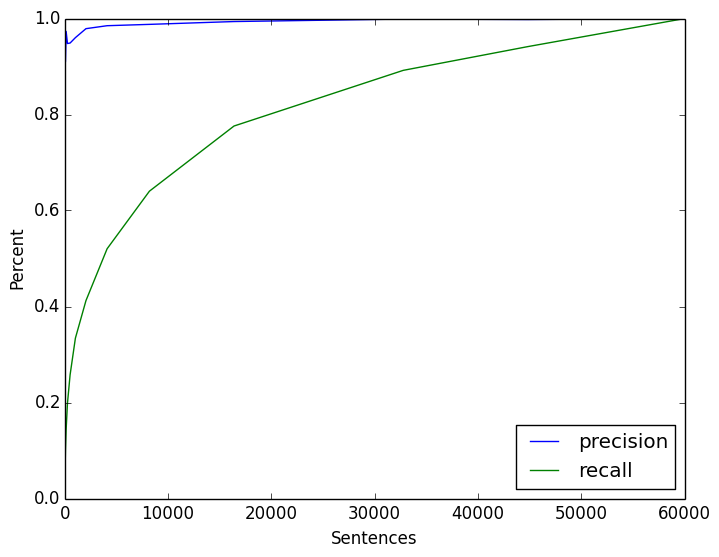
\includegraphics[width=\linewidth, keepaspectratio=true]{figure/precision_recall.png}
  \caption{Convergence to the direction mapping obtained on the largest run.  Precision relative to that run is very high even for small datasets.  Recall grows as more link types are seen.}\label{fig:convergence}
\end{figure}

We worried that the direction mapping might be unstable and sensitive to the input corpus.  Figure~\ref{fig:convergence} shows otherwise (for both English and Russian). \noteJE{IMPORTANT! current graph is with fine-grained tags; rerun with the coarse-grained tags as in the rest of the paper} Using even a small prefix of the data got very high-precision results, in the sense that nearly all $r_L$ or $\ell_L$ variables that were 1 in this lightly trained mapping were also 1 in our largest run.  The only disadvantage to using small data is low recall relative to the large run---many of the labels $L$ are not observed yet and so we do not yet allow either direction ($r_L=\ell_L=0$).  

We used only coarse link tags as our labels, keeping only the capital letters of a tag (and merging all \texttt{ID} tags).  This is because other characters in a tag indicate fine-grained features such as plurality that generally do not affect link direction.  However, when we tried using fine tags as our labels instead, we found that all refinements of the same coarse tag would almost always spontaneously agree on their preferred direction.  This indicates that there is indeed a ``natural'' direction for the coarse tag and that we can find it.

% OLD
% We report on the convergence of the results of our ILP with increasing data. With increasing trials of sentences, we measure how similar the subsequent direction mappings would be with each other. Taking the direction table of the largest run as the answer key, we compared how much the solutions of the smaller runs deviated from it. 
% We recorded the precision of whether the mappings in the smaller runs could be found in those of the largest run, and similarly the recall of whether the mappings in the largest run could be found in the smaller runs. 

% Because the precision values were high, we found that the solutions of the previous runs were consistent with the largest run, and as the data increased so did the recall values, and so we would continue to encounter novel link types and then incorporate them.

\subsection{Linguistic Analysis}

The resulting English corpus uses a syntactic annotation scheme that is somewhat different from the CoNLL annotations.  Differences are tabulated in Appendix~\ref{app:linktypes}, and the actual parses are contrasted in Figure~\ref{fig:parses} and Appendix~\ref{app:parses}.

The link grammar results in multi-headed treatments of infinitivals, compound determiners, relative clauses, and embedding.  The other annotation differences are generally reasonable, e.g., letting {\em 's} be the head of a possessive, and different handling of punctuation and lists.  Of course, a few of the differences are due to parser attachment errors.

The most vexing issue is that subject-verb links are handled inconsistently.  Under the English link grammar, a verb that governs a clause (or 0 for the main clause) will link to both the clause's subject and its last (main) verb.  This ought to give us the desired treatment of {\em ``Jill persuaded him to skip''}, in which {\em ``him''} has two parents.  Unfortunately, the grammar is inconsistent when the subject is missing ({\em ``Jill wanted to skip''}): the governing verb here links instead to the clause's first (tensed) verb but {\em no longer} to the last as well.  This favors a consistent solution where each auxiliary verb is a parent of the verb to its right ({\em to} $\rightarrow$ {\em skip}).  As a result, when the subject is present, it must be the {\em parent} of the first verb, which otherwise would not have a parent ({\em him} $\rightarrow$ {\em to} $\rightarrow$ {\em skip}).  Yet inconsistently, subjects must be {\em children} of verbs in a few  inconsistently handled constructions such as non-embedded reported speech ({\em ``It was impossible, they said''}), since the subject ({\em ``they''}) links only to the verb ({\em ``said''}) and so has no other possible parent.


% Multiheaded:
% IV (890/891) - multiheaded treatment of infinitivals
% I (1783/2969) - multiheaded treatment of infinitivals
% B (795/842) - leftward extraction from relative clauses
% CV (1588/1799) - multiheaded treatment of subordination
% AL (39/40) - compound determiners
% PP (448/689) - subject attaches to aux as well as main verb
% HA (3/3) -
% JQ (2/2) - 
% SF (85/111) - pleonastic subject
% AF (6/12) - 
% C (244/1813) - 
% OF (155/291)
% P (651/2060) - 
% Q (12/30)- 
% RS (300/305) - 
% S (4256/7434) -
% SX (4/6) - 
% W (2321/4721) - 
% WV (1800/4138) - 

\NoteJE{what do we say about Russian?  ask Ryan for final version?}


% DOESN'T SEEM NECESSARY FOR THE LANGUAGES WE TRIED
% \section{Future Work}
% \subsection{Slack Hierarchy}
% We would like to introduce slack on the link grammar types such that link types with the same coarse grained label would try and align the same way as the majority in the group, where the preceding capital letters of the link type denote the coarse grained label, while the subscript letters denote further information. This slack would place a prior on rare or never-before seen link types to be assigned in the same way as other similar link types. We think that this will give the ILP better flexibility to handle noise and novel link types while still trying to learn the overall link grammar.


\newpage
\bibliographystyle{acl2014}
\bibliography{LinksToDAG}


\appendix
\clearpage
\onecolumn

% OLD
% \section{ILP Formulation}
% We present our ILP formulation. 
% 
% \begin{figure}[!htb]
%   \small
%   \begin{align*}
%     \text{Sets:}&&\\
%     &\textsc{link}_{\textsc{sentence},\textsc{label}, i,j} \in \textsc{links} &\\
%     &\textsc{label} \in \textsc{labels}&\\ 
%     &\textsc{dir} = \{\textsc{left}, \textsc{right}\} &\\
%     \text{Params:}&&\\
%     &\textsc{m}_\textsc{length} = \max (\forall{\textsc{link}_{\textsc{sentence}, i,j}} \max(i,j)) &\\
%     %&\textsc{count}_{\textsc{label}, \textsc{dir}} = \sum_{\textsc{link}_{\textsc{label},\textsc{dir}}}1 &\\
%     &\textsc{cost}_{\textsc{label}} = \frac{100}{ \sum_{\textsc{link}_{\textsc{label},\textsc{dir}}}1 } &\\
%     \text{Variables:}&&\\
%     &\textsc{slack}_{\textsc{link}} \geq 0 &\\ 
%     &\textsc{depth}_{\textsc{sentence},i} \geq 0 &\\
%     &\textsc{allowed}_{\textsc{label},\textsc{dir}} = \{0,1\}&\\
%     &\textsc{arc}_{\textsc{link}} = \{0,1\} &\\
%     \text{minimize:}& &\\ 
%     &\sum_{\textsc{label}, \textsc{dir}} (\textsc{allowed}_{\textsc{label},\textsc{dir}}) + \textsc{cost}_{\textsc{label}} \cdot \sum_\textsc{link} \textsc{slack}_{\textsc{link}} &\\
%     &&\\
%     \text{subject to: }& &\\
%     &\text{Links go in the allowed directions, except for slack}&\\
%     &\forall{\textsc{link}_{i,j,\textsc{label}}}: 1-\textsc{arc}_{\textsc{link}} \leq \textsc{allowed}_{\textsc{label}, \textsc{left}} + \textsc{slack}_{\textsc{link}} &\\
%     &\forall{\textsc{link}_{i,j,\textsc{label}}}: \textsc{arc}_{\textsc{link}} \leq \textsc{allowed}_{\textsc{label}, \textsc{right}} + \textsc{slack}_{\textsc{link}} &\\
%     &\text{Depth constraints for acyclicity}&\\
%     &\forall{\textsc{link}_{\textsc{sentence},i}}: \textsc{depth}_{\textsc{sentence},\text{root}} \leq \textsc{depth}_{\textsc{sentence},i} &\\
%     &\forall{\textsc{link}_{\textsc{sentence},i,j}}: \textsc{depth}_{\textsc{sentence},i} + \textsc{m}_\textsc{length}\cdot\textsc{arc}_{\textsc{sentence},i,j} \geq \textsc{depth}_{\textsc{sentence},j} + 1 &\\
%     &\forall{\textsc{link}_{\textsc{sentence},i,j}}: \textsc{depth}_{\textsc{sentence},j} + \textsc{m}_\textsc{length}\cdot(1-\textsc{arc}_{\textsc{sentence},i,j}) \geq \textsc{depth}_{\textsc{sentence},i} + 1 &\\
%     &\text{Every token has a parent}&\\
%     &\forall{\textsc{link}_{\textsc{sentence},i \neq \textsc{root}}}: \sum_{\textsc{link}_{\textsc{sentence},i,j}} (1-\textsc{arc}_{\textsc{sentence},i,j}) + \sum_{\textsc{link}_{\textsc{sentence},j,i}}(\textsc{arc}_{\textsc{sentence},j,i}) \geq 1&\\
%   \end{align*}
%   \caption{\small The ILP formulation.}
% \end{figure}
% 
% 
% \clearpage

\section{English Link Types}\label{app:linktypes}

Recall that \url{http://www.abisource.com/projects/link-grammar/dict/summarize-links.html} documents the 122 link types in the English link grammar lexicon.  Below is the result of our largest English run, whose corpus uses !!! of these types.  

Other researchers could postprocess link grammar parses by using the first two columns.  These indicate whether a given link label $L$ tended to be oriented rightward or leftward by our ILP.  

The labels that do not have a consistent direction are mainly those that connect a conjunction to its conjuncts.\footnote{See \url{http://www.abisource.com/projects/link-grammar/dict/coordination.html}.}  
Our coarsening of the labels (see section~\ref{sec:stability}) discarded the characters that distinguish left from right conjuncts.

The third column indicates where multi-headedness happens, by showing how often the child of an $L$ link had additional parents as well.

The remaining columns compare to the CoNLL parses.  They show the fraction of $L$-labeled link tokens that were also present in the CoNLL reference parse---and on that fraction, whether the orientation matches CoNLL's and what the dominant CoNLL label was.

\NoteJE{improve table formatting.  Numeric justification; en dashes; longtable; remove most hlines.}

\renewcommand{\arraystretch}{1.2}    % more space between rows
\begin{small}
\centering
\begin{longtable}{|l|l|l|l|l|l|}
\hline
Label & Rightward & Multiheaded & CoNLL Match & CoNLL Dir Match & CoNLL Label\\ 
\hline
A & 0\% (0/426) & 0\% (0/426) & 86\% (365/426) & 99\% (360/365) & NMOD 99\% (360/365) \\ 
\hline
AF & 100\% (1/1) & 100\% (1/1) & 100\% (1/1) & 0\% (0/1) & VMOD 100\% (1/1) \\ 
\hline
AJ & 50\% (10/20) & 0\% (0/20) & 75\% (15/20) & 100\% (15/15) & COORD 93\% (14/15) \\ 
\hline
AL & 100\% (8/8) & 100\% (8/8) & - & - & - \\ 
\hline
AM & 0\% (0/2) & 0\% (0/2) & - & - & - \\ 
\hline
AN & 0\% (0/426) & 0\% (0/426) & 83\% (353/426) & 98\% (347/353) & NMOD 99\% (348/353) \\ 
\hline
B & 100\% (77/77) & 56\% (43/77) & 60\% (46/77) & 87\% (40/46) & NMOD 72\% (33/46) \\ 
\hline
BI & 100\% (4/4) & 0\% (0/4) & 25\% (1/4) & 100\% (1/1) & VMOD 100\% (1/1) \\ 
\hline
C & 100\% (128/128) & 2\% (2/128) & 3\% (4/128) & 50\% (2/4) & NMOD 75\% (3/4) \\ 
\hline
CC & 100\% (5/5) & 0\% (0/5) & - & - & - \\ 
\hline
CO & 0\% (0/119) & 3\% (4/119) & 8\% (9/119) & 100\% (9/9) & NMOD 78\% (7/9) \\ 
\hline
CP & 100\% (26/26) & 4\% (1/26) & 92\% (24/26) & 100\% (24/24) & ROOT 100\% (24/24) \\ 
\hline
CV & 100\% (127/127) & 98\% (125/127) & 54\% (68/127) & 26\% (18/68) & VMOD 47\% (32/68) \\ 
\hline
D & 0\% (3/1048) & 1\% (8/1048) & 88\% (917/1048) & 100\% (915/917) & NMOD 100\% (916/917) \\ 
\hline
DD & 0\% (0/30) & 0\% (0/30) & 30\% (9/30) & 100\% (9/9) & NMOD 100\% (9/9) \\ 
\hline
DG & 0\% (0/64) & 0\% (0/64) & 91\% (58/64) & 100\% (58/58) & NMOD 100\% (58/58) \\ 
\hline
DP & 0\% (0/1) & 0\% (0/1) & 100\% (1/1) & 100\% (1/1) & SBJ 100\% (1/1) \\ 
\hline
DT & 0\% (0/21) & 0\% (0/21) & 100\% (21/21) & 100\% (21/21) & NMOD 100\% (21/21) \\ 
\hline
E & 0\% (0/103) & 0\% (0/103) & 74\% (76/103) & 96\% (73/76) & ADV 79\% (60/76) \\ 
\hline
EA & 0\% (0/24) & 0\% (0/24) & 92\% (22/24) & 100\% (22/22) & AMOD 95\% (21/22) \\ 
\hline
EB & 100\% (19/19) & 0\% (0/19) & 63\% (12/19) & 92\% (11/12) & VMOD 75\% (9/12) \\ 
\hline
EC & 0\% (0/1) & 0\% (0/1) & 100\% (1/1) & 100\% (1/1) & AMOD 100\% (1/1) \\ 
\hline
EE & 0\% (0/4) & 0\% (0/4) & 100\% (4/4) & 25\% (1/4) & AMOD 100\% (4/4) \\ 
\hline
EF & 100\% (1/1) & 0\% (0/1) & 100\% (1/1) & 0\% (0/1) & AMOD 100\% (1/1) \\ 
\hline
EN & 0\% (0/22) & 0\% (0/22) & 77\% (17/22) & 24\% (4/17) & AMOD 76\% (13/17) \\ 
\hline
G & 0\% (0/305) & 0\% (0/305) & 69\% (211/305) & 98\% (206/211) & NMOD 94\% (199/211) \\ 
\hline
GN & 0\% (0/12) & 0\% (0/12) & 83\% (10/12) & 100\% (10/10) & NMOD 100\% (10/10) \\ 
\hline
H & 100\% (1/1) & 0\% (0/1) & 100\% (1/1) & 100\% (1/1) & AMOD 100\% (1/1) \\ 
\hline
I & 100\% (266/267) & 63\% (167/267) & 94\% (252/267) & 51\% (128/252) & VC 48\% (122/252) \\ 
\hline
ID & 0\% (0/76) & 0\% (0/76) & 74\% (56/76) & 36\% (20/56) & AMOD 38\% (21/56) \\ 
\hline
IN & 100\% (9/9) & 0\% (0/9) & 100\% (9/9) & 100\% (9/9) & PMOD 100\% (9/9) \\ 
\hline
IV & 100\% (73/73) & 100\% (73/73) & 81\% (59/73) & 92\% (54/59) & OBJ 61\% (36/59) \\ 
\hline
J & 99\% (844/856) & 1\% (12/856) & 87\% (741/856) & 96\% (714/741) & PMOD 97\% (720/741) \\ 
\hline
JG & 100\% (2/2) & 0\% (0/2) & 50\% (1/2) & 100\% (1/1) & PMOD 100\% (1/1) \\ 
\hline
JT & 100\% (1/1) & 0\% (0/1) & 100\% (1/1) & 100\% (1/1) & AMOD 100\% (1/1) \\ 
\hline
K & 100\% (28/28) & 0\% (0/28) & 100\% (28/28) & 100\% (28/28) & ADV 54\% (15/28) \\ 
\hline
L & 100\% (27/27) & 0\% (0/27) & - & - & - \\ 
\hline
M & 100\% (495/495) & 0\% (0/495) & 75\% (372/495) & 94\% (351/372) & NMOD 84\% (311/372) \\ 
\hline
MG & 100\% (2/2) & 0\% (0/2) & 50\% (1/2) & 100\% (1/1) & NMOD 100\% (1/1) \\ 
\hline
MJ & 50\% (7/14) & 0\% (0/14) & 79\% (11/14) & 100\% (11/11) & COORD 91\% (10/11) \\ 
\hline
MV & 100\% (672/672) & 0\% (2/672) & 54\% (366/672) & 99\% (363/366) & ADV 77\% (280/366) \\ 
\hline
MX & 100\% (105/105) & 4\% (4/105) & 39\% (41/105) & 88\% (36/41) & NMOD 88\% (36/41) \\ 
\hline
N & 100\% (29/29) & 0\% (0/29) & 100\% (29/29) & 100\% (29/29) & VMOD 100\% (29/29) \\ 
\hline
NA & 0\% (0/2) & 0\% (0/2) & 100\% (2/2) & 50\% (1/2) & COORD 100\% (2/2) \\ 
\hline
ND & 0\% (0/29) & 0\% (0/29) & 72\% (21/29) & 100\% (21/21) & NMOD 71\% (15/21) \\ 
\hline
NI & 33\% (4/12) & 0\% (0/12) & 67\% (8/12) & 100\% (8/8) & NMOD 50\% (4/8) \\ 
\hline
NM & 100\% (31/31) & 0\% (0/31) & 84\% (26/31) & 69\% (18/26) & AMOD 69\% (18/26) \\ 
\hline
NN & 0\% (0/21) & 0\% (0/21) & 33\% (7/21) & 100\% (7/7) & AMOD 100\% (7/7) \\ 
\hline
NS & 0\% (0/9) & 0\% (0/9) & 78\% (7/9) & 100\% (7/7) & NMOD 100\% (7/7) \\ 
\hline
NT & 0\% (0/2) & 0\% (0/2) & - & - & - \\ 
\hline
O & 100\% (576/576) & 0\% (0/576) & 81\% (465/576) & 97\% (450/465) & OBJ 72\% (336/465) \\ 
\hline
OD & 100\% (2/2) & 0\% (0/2) & 100\% (2/2) & 100\% (2/2) & ADV 50\% (1/2) \\ 
\hline
OF & 100\% (24/24) & 50\% (12/24) & 100\% (24/24) & 96\% (23/24) & NMOD 67\% (16/24) \\ 
\hline
OT & 100\% (1/1) & 0\% (0/1) & 100\% (1/1) & 100\% (1/1) & OBJ 100\% (1/1) \\ 
\hline
P & 99\% (189/190) & 34\% (65/190) & 94\% (179/190) & 99\% (178/179) & VC 56\% (101/179) \\ 
\hline
\end{longtable}
\end{small}
\begin{small}
\centering
\begin{longtable}{|l|l|l|l|l|l|}
\hline
Label & Rightward & Multiheaded & CoNLL Match & CoNLL Dir Match & CoNLL Label\\ 
\hline
PP & 98\% (57/58) & 71\% (41/58) & 95\% (55/58) & 100\% (55/55) & VC 100\% (55/55) \\ 
\hline
Q & 100\% (3/3) & 33\% (1/3) & 100\% (3/3) & 67\% (2/3) & ROOT 67\% (2/3) \\ 
\hline
QI & 100\% (8/8) & 0\% (0/8) & 13\% (1/8) & 100\% (1/1) & PMOD 100\% (1/1) \\ 
\hline
R & 100\% (68/68) & 49\% (33/68) & 15\% (10/68) & 30\% (3/10) & NMOD 60\% (6/10) \\ 
\hline
RJ & 0\% (0/4) & 50\% (2/4) & - & - & - \\ 
\hline
RS & 0\% (0/33) & 100\% (33/33) & 100\% (33/33) & 100\% (33/33) & SBJ 100\% (33/33) \\ 
\hline
S & 95\% (636/671) & 56\% (378/671) & 91\% (612/671) & 8\% (46/612) & SBJ 97\% (593/612) \\ 
\hline
SF & 100\% (11/11) & 82\% (9/11) & 82\% (9/11) & 0\% (0/9) & SBJ 100\% (9/9) \\ 
\hline
SFI & 100\% (1/1) & 0\% (0/1) & 100\% (1/1) & 100\% (1/1) & SBJ 100\% (1/1) \\ 
\hline
SI & 100\% (4/4) & 0\% (0/4) & 100\% (4/4) & 100\% (4/4) & SBJ 100\% (4/4) \\ 
\hline
SJ & 50\% (155/310) & 0\% (0/310) & 68\% (212/310) & 91\% (193/212) & COORD 84\% (179/212) \\ 
\hline
SX & 100\% (2/2) & 100\% (2/2) & 100\% (2/2) & 0\% (0/2) & SBJ 100\% (2/2) \\ 
\hline
TA & 0\% (0/2) & 0\% (0/2) & 100\% (2/2) & 100\% (2/2) & NMOD 100\% (2/2) \\ 
\hline
TH & 100\% (21/21) & 0\% (0/21) & - & - & - \\ 
\hline
TI & 100\% (2/2) & 0\% (0/2) & 100\% (2/2) & 100\% (2/2) & PMOD 50\% (1/2) \\ 
\hline
TM & 100\% (1/1) & 0\% (0/1) & 100\% (1/1) & 100\% (1/1) & NMOD 100\% (1/1) \\ 
\hline
TO & 100\% (82/82) & 0\% (0/82) & 1\% (1/82) & 100\% (1/1) & NMOD 100\% (1/1) \\ 
\hline
TY & 100\% (3/3) & 0\% (0/3) & 100\% (3/3) & 100\% (3/3) & NMOD 100\% (3/3) \\ 
\hline
U & 100\% (3/3) & 0\% (0/3) & 100\% (3/3) & 100\% (3/3) & PMOD 100\% (3/3) \\ 
\hline
VJ & 51\% (46/90) & 0\% (0/90) & 61\% (55/90) & 78\% (43/55) & COORD 78\% (43/55) \\ 
\hline
W & 100\% (546/546) & 0\% (0/546) & 4\% (23/546) & 52\% (12/23) & P 48\% (11/23) \\ 
\hline
WN & 100\% (1/1) & 0\% (0/1) & - & - & - \\ 
\hline
WV & 100\% (426/426) & 100\% (426/426) & 56\% (237/426) & 97\% (230/237) & ROOT 97\% (230/237) \\ 
\hline
X & 79\% (679/863) & 6\% (53/863) & 10\% (86/863) & 94\% (81/86) & P 100\% (86/86) \\ 
\hline
Y & 0\% (0/4) & 0\% (0/4) & 75\% (3/4) & 100\% (3/3) & AMOD 100\% (3/3) \\ 
\hline
YP & 0\% (0/7) & 0\% (0/7) & 100\% (7/7) & 0\% (0/7) & NMOD 100\% (7/7) \\ 
\hline
YS & 0\% (0/65) & 0\% (0/65) & 98\% (64/65) & 0\% (0/64) & NMOD 100\% (64/64) \\ 
\hline
Z & 100\% (1/1) & 0\% (0/1) & - & - & - \\ 
\hline
\end{longtable}
\end{small}


\section{Sample English Parses}\label{app:parses}

\NoteJE{show the fine-grained link labels in the parses, even though the ILP deals with coarse-grained.  Juneki tried already to hack this in but was getting double links.}

Below we display the first 100 English sentences whose widths do not exceed the width of this page.  The blue upper half shows the CoNLL tagging and dependency parse.  The red lower half shows the link grammar's tagging and our orientation of the link parse.  
% The dashes in the link grammar part of speech tag annotations mean that the link parser did not return one.
A vertical edge to word token $v$ denotes an edge $0 \rightarrow v$.
Words that were unknown to the link parser are flagged with \texttt{[!]}.  

Edges are shown as solid lines if they appear in both parses.  They are drawn more thickly if the directions do not match.

Edges are shown as dotted lines if they appear only in one parse and not in the other.  Such edges are highlighted in orange if the child has multiple parents.  

% OLD
% For every arc:
% \begin{enumerate}
% \item If there is a corresponding link between the same nodes then a solid blue line is drawn.
% \item Or else a dotted blue line is drawn. 
% \end{enumerate}
% The bottom red arcs represent the oriented link grammar parses. For every link edge:
% \begin{enumerate}
% \item If there is a corresponding CoNLL arc between the same nodes then a solid red line is drawn.
% \item If the matching arc is facing the opposite direction, then the link edge is drawn thicker.
% \item Of the remaining edges, if an edge is a multiheaded link, then it is drawn with thick orange.
% \item The rest of the remaining edges are drawn with dotted red lines.
% \end{enumerate}

% \subsection{Link Parser Annotations}
% These sentences have been taken from the English bnews training data set. We chose to display sentences with complete link parses similar to the analysis section of this paper. 
% 
% \subsection{Parse Colorization}
% The sentence used in the middle of the parse is taken from the output of the link parser. We removed sentences with dropped words, but they would have shown up in the parse as [bracketed]. 



% Uncomment this to add in all of the parses. Warning: compilation will take a long time.
%\begin{figure*}[ht!]
	\begin{dependency}
		\begin{deptext}
			{\scriptsize PR} \& {\scriptsize VB} \& {\scriptsize VB} \& {\scriptsize DT} \& {\scriptsize NN} \& {\scriptsize PR} \& {\scriptsize VB} \& {\scriptsize TO} \& {\scriptsize VB} \& {\scriptsize IN} \& {\scriptsize VB} \& {\scriptsize IN} \& {\scriptsize JJ} \& {\scriptsize NN} \& {\scriptsize .} \\
			they \& chance \& alienating \& the \& customers \& they \& hope \& to \& woo \& by \& looking \& like \& opportunistic \& sharks \& . \\
			- \& v \& g \& - \& n \& - \& v \& r \& v \& - \& v \& p \& a \& n \& - \\
		\end{deptext}
		\depedge[edge below, edge style = {red, thick}]{11}{12}{MV}
		\depedge[edge above, edge style = {blue, thick}]{11}{12}{\small ADV}
		\depedge[edge below, edge style = {red, thick}]{10}{11}{M}
		\depedge[edge above, edge style = {blue, thick}]{10}{11}{\small PMOD}
		\depedge[edge below, edge style = {red, thick}]{12}{14}{J}
		\depedge[edge above, edge style = {blue, thick}]{12}{14}{\small PMOD}
		\depedge[edge below, edge style = {red, thick}]{14}{13}{A}
		\depedge[edge above, edge style = {blue, thick}]{14}{13}{\small NMOD}
		\deproot[edge below, edge style = {orange, thick}]{2}{WV}
		\deproot[edge above, edge style = {blue, thick}]{2}{\small ROOT}
		\depedge[edge below, edge style = {red, thick}]{3}{5}{R}
		\depedge[edge above, edge style = {blue, thick}]{3}{5}{\small OBJ}
		\depedge[edge above, edge style = {blue, dotted}]{3}{10}{\small ADV}
		\depedge[edge below, edge style = {orange, ultra thick}]{1}{2}{S}
		\depedge[edge above, edge style = {blue, ultra thick}]{2}{1}{\small SBJ}
		\depedge[edge below, edge style = {red, thick}]{2}{3}{O}
		\depedge[edge above, edge style = {blue, thick}]{2}{3}{\small OBJ}
		\depedge[edge above, edge style = {blue, dotted}]{2}{15}{\small P}
		\depedge[edge below, edge style = {red, thick}]{5}{4}{D}
		\depedge[edge above, edge style = {blue, thick}]{5}{4}{\small NMOD}
		\depedge[edge above, edge style = {blue, dotted}]{5}{7}{\small NMOD}
		\depedge[edge below, edge style = {red, ultra thick}]{6}{7}{S}
		\depedge[edge above, edge style = {blue, ultra thick}]{7}{6}{\small SBJ}
		\depedge[edge above, edge style = {blue, dotted}]{7}{9}{\small OBJ}
		\depedge[edge above, edge style = {blue, dotted}]{9}{8}{\small VMOD}
		\deproot[edge below, edge style = {red, dotted}]{1}{W}
		\deproot[edge below, edge style = {red, dotted}]{15}{X}
		\depedge[edge below, edge style = {orange, ultra thick, dotted}]{3}{9}{B}
		\depedge[edge below, edge style = {red, dotted}]{5}{6}{R}
		\depedge[edge below, edge style = {orange, ultra thick, dotted}]{5}{8}{B}
		\depedge[edge below, edge style = {orange, ultra thick, dotted}]{5}{9}{S}
		\depedge[edge below, edge style = {orange, ultra thick, dotted}]{7}{8}{MV}
		\depedge[edge below, edge style = {red, dotted}]{9}{10}{MV}
	\end{dependency}
\end{figure*}

\begin{figure*}[ht!]
	\begin{dependency}
		\begin{deptext}
			{\scriptsize DT} \& {\scriptsize NN} \& {\scriptsize VB} \& {\scriptsize DT} \& {\scriptsize NN} \& {\scriptsize IN} \& {\scriptsize NN} \& {\scriptsize IN} \& {\scriptsize DT} \& {\scriptsize NN} \& {\scriptsize IN} \& {\scriptsize NN} \& {\scriptsize .} \\
			the \& companies \& reached \& an \& agreement \& in \& principle \& for \& the \& sale \& in \& August \& . \\
			- \& n \& v-d \& - \& s \& r \& n \& p \& - \& n-u \& r \& i \& - \\
		\end{deptext}
		\depedge[edge below, edge style = {red, thick}]{11}{12}{IN}
		\depedge[edge above, edge style = {blue, thick}]{11}{12}{\small PMOD}
		\depedge[edge below, edge style = {red, thick}]{10}{9}{D}
		\depedge[edge above, edge style = {blue, thick}]{10}{9}{\small NMOD}
		\deproot[edge below, edge style = {orange, thick}]{3}{WV}
		\deproot[edge above, edge style = {blue, thick}]{3}{\small ROOT}
		\depedge[edge below, edge style = {orange, ultra thick}]{2}{3}{S}
		\depedge[edge above, edge style = {blue, ultra thick}]{3}{2}{\small SBJ}
		\depedge[edge below, edge style = {red, thick}]{3}{5}{O}
		\depedge[edge above, edge style = {blue, thick}]{3}{5}{\small OBJ}
		\depedge[edge below, edge style = {red, thick}]{3}{11}{MV}
		\depedge[edge above, edge style = {blue, thick}]{3}{11}{\small ADV}
		\depedge[edge above, edge style = {blue, dotted}]{3}{13}{\small P}
		\depedge[edge below, edge style = {red, thick}]{2}{1}{D}
		\depedge[edge above, edge style = {blue, thick}]{2}{1}{\small NMOD}
		\depedge[edge below, edge style = {red, thick}]{5}{4}{D}
		\depedge[edge above, edge style = {blue, thick}]{5}{4}{\small NMOD}
		\depedge[edge above, edge style = {blue, dotted}]{5}{6}{\small NMOD}
		\depedge[edge above, edge style = {blue, dotted}]{5}{8}{\small NMOD}
		\depedge[edge below, edge style = {red, thick}]{6}{7}{J}
		\depedge[edge above, edge style = {blue, thick}]{6}{7}{\small PMOD}
		\depedge[edge below, edge style = {red, thick}]{8}{10}{J}
		\depedge[edge above, edge style = {blue, thick}]{8}{10}{\small PMOD}
		\deproot[edge below, edge style = {red, dotted}]{2}{W}
		\deproot[edge below, edge style = {red, dotted}]{13}{X}
		\depedge[edge below, edge style = {red, dotted}]{3}{6}{MV}
		\depedge[edge below, edge style = {red, dotted}]{7}{8}{M}
	\end{dependency}
\end{figure*}

\begin{figure*}[ht!]
	\begin{dependency}
		\begin{deptext}
			{\scriptsize IN} \& {\scriptsize DT} \& {\scriptsize RB} \& {\scriptsize CD} \& {\scriptsize NN} \& {\scriptsize VB} \& {\scriptsize ,} \& {\scriptsize CD} \& {\scriptsize VB} \& {\scriptsize DT} \& {\scriptsize NN} \& {\scriptsize TO} \& {\scriptsize VB} \& {\scriptsize .} \\
			of \& the \& almost \& 3{,}000\lbrack !\rbrack \& athletes \& surveyed \& {,} \& 1{,}240\lbrack !\rbrack \& took \& the \& time \& to \& respond \& . \\
			- \& - \& - \& - \& n \& v-d \& - \& - \& v-d \& - \& n \& r \& v \& - \\
		\end{deptext}
		\depedge[edge below, edge style = {red, thick}]{11}{10}{D}
		\depedge[edge above, edge style = {blue, thick}]{11}{10}{\small NMOD}
		\depedge[edge below, edge style = {orange, thick}]{11}{13}{IV}
		\depedge[edge above, edge style = {blue, thick}]{11}{13}{\small NMOD}
		\depedge[edge below, edge style = {orange, ultra thick}]{12}{13}{I}
		\depedge[edge above, edge style = {blue, ultra thick}]{13}{12}{\small VMOD}
		\depedge[edge below, edge style = {red, thick}]{1}{5}{J}
		\depedge[edge above, edge style = {blue, thick}]{1}{5}{\small PMOD}
		\deproot[edge below, edge style = {orange, thick}]{9}{WV}
		\deproot[edge above, edge style = {blue, thick}]{9}{\small ROOT}
		\depedge[edge below, edge style = {red, ultra thick}]{4}{3}{EN}
		\depedge[edge above, edge style = {blue, ultra thick}]{3}{4}{\small AMOD}
		\depedge[edge above, edge style = {blue, dotted}]{5}{2}{\small NMOD}
		\depedge[edge above, edge style = {blue, dotted}]{5}{3}{\small NMOD}
		\depedge[edge above, edge style = {blue, dotted}]{5}{6}{\small NMOD}
		\depedge[edge above, edge style = {blue, dotted}]{9}{1}{\small VMOD}
		\depedge[edge above, edge style = {blue, dotted}]{9}{7}{\small P}
		\depedge[edge below, edge style = {orange, ultra thick}]{8}{9}{S}
		\depedge[edge above, edge style = {blue, ultra thick}]{9}{8}{\small SBJ}
		\depedge[edge below, edge style = {red, thick}]{9}{11}{O}
		\depedge[edge above, edge style = {blue, thick}]{9}{11}{\small OBJ}
		\depedge[edge above, edge style = {blue, dotted}]{9}{14}{\small P}
		\depedge[edge below, edge style = {red, dotted}]{11}{12}{TO}
		\deproot[edge below, edge style = {red, dotted}]{8}{W}
		\deproot[edge below, edge style = {red, dotted}]{14}{X}
		\depedge[edge below, edge style = {red, dotted}]{5}{4}{D}
		\depedge[edge below, edge style = {red, dotted}]{4}{2}{DD}
		\depedge[edge below, edge style = {red, dotted}]{6}{7}{X}
		\depedge[edge below, edge style = {red, dotted}]{8}{1}{CO}
		\depedge[edge below, edge style = {red, dotted}]{8}{6}{CO}
	\end{dependency}
\end{figure*}

\begin{figure*}[ht!]
	\begin{dependency}
		\begin{deptext}
			{\scriptsize IN} \& {\scriptsize DT} \& {\scriptsize CD} \& {\scriptsize NN} \& {\scriptsize ,} \& {\scriptsize CD} \& {\scriptsize NN} \& {\scriptsize VB} \& {\scriptsize VB} \& {\scriptsize DT} \& {\scriptsize NN} \& {\scriptsize NN} \& {\scriptsize .} \\
			since \& that \& 1976\lbrack !\rbrack \& ruling \& {,} \& 37 \& states \& have \& reintroduced \& the \& death \& penalty \& . \\
			- \& j-d \& - \& n \& - \& - \& n \& v \& v \& - \& s \& n-u \& - \\
		\end{deptext}
		\depedge[edge below, edge style = {red, thick}]{12}{10}{D}
		\depedge[edge above, edge style = {blue, thick}]{12}{10}{\small NMOD}
		\depedge[edge below, edge style = {red, thick}]{12}{11}{AN}
		\depedge[edge above, edge style = {blue, thick}]{12}{11}{\small NMOD}
		\depedge[edge below, edge style = {red, thick}]{1}{4}{J}
		\depedge[edge above, edge style = {blue, thick}]{1}{4}{\small PMOD}
		\deproot[edge above, edge style = {blue, dotted}]{8}{\small ROOT}
		\depedge[edge below, edge style = {red, thick}]{4}{2}{D}
		\depedge[edge above, edge style = {blue, thick}]{4}{2}{\small NMOD}
		\depedge[edge below, edge style = {red, thick}]{4}{3}{AN}
		\depedge[edge above, edge style = {blue, thick}]{4}{3}{\small NMOD}
		\depedge[edge below, edge style = {red, thick}]{7}{6}{D}
		\depedge[edge above, edge style = {blue, thick}]{7}{6}{\small NMOD}
		\depedge[edge below, edge style = {red, thick}]{9}{12}{O}
		\depedge[edge above, edge style = {blue, thick}]{9}{12}{\small OBJ}
		\depedge[edge above, edge style = {blue, dotted}]{8}{1}{\small ADV}
		\depedge[edge above, edge style = {blue, dotted}]{8}{5}{\small P}
		\depedge[edge below, edge style = {red, ultra thick}]{7}{8}{S}
		\depedge[edge above, edge style = {blue, ultra thick}]{8}{7}{\small SBJ}
		\depedge[edge below, edge style = {orange, thick}]{8}{9}{PP}
		\depedge[edge above, edge style = {blue, thick}]{8}{9}{\small VC}
		\depedge[edge above, edge style = {blue, dotted}]{8}{13}{\small P}
		\depedge[edge below, edge style = {red, dotted}]{1}{5}{X}
		\deproot[edge below, edge style = {red, dotted}]{7}{W}
		\deproot[edge below, edge style = {orange, ultra thick, dotted}]{9}{WV}
		\deproot[edge below, edge style = {red, dotted}]{13}{X}
		\depedge[edge below, edge style = {red, dotted}]{7}{1}{CO}
	\end{dependency}
\end{figure*}

\begin{figure*}[ht!]
	\begin{dependency}
		\begin{deptext}
			{\scriptsize NN} \& {\scriptsize NN} \& {\scriptsize RB} \& {\scriptsize VB} \& {\scriptsize DT} \& {\scriptsize NN} \& {\scriptsize IN} \& {\scriptsize VB} \& {\scriptsize NN} \& {\scriptsize .} \\
			Mr. \& Bakes\lbrack !\rbrack \& previously \& had \& a \& turn \& at \& running \& Continental\lbrack !\rbrack \& . \\
			x \& - \& - \& v-d \& - \& n \& - \& v \& - \& - \\
		\end{deptext}
		\deproot[edge below, edge style = {orange, thick}]{4}{WV}
		\deproot[edge above, edge style = {blue, thick}]{4}{\small ROOT}
		\depedge[edge below, edge style = {red, thick}]{2}{1}{G}
		\depedge[edge above, edge style = {blue, thick}]{2}{1}{\small NMOD}
		\depedge[edge below, edge style = {orange, ultra thick}]{2}{4}{S}
		\depedge[edge above, edge style = {blue, ultra thick}]{4}{2}{\small SBJ}
		\depedge[edge below, edge style = {red, thick}]{4}{3}{E}
		\depedge[edge above, edge style = {blue, thick}]{4}{3}{\small ADV}
		\depedge[edge below, edge style = {red, thick}]{4}{6}{O}
		\depedge[edge above, edge style = {blue, thick}]{4}{6}{\small OBJ}
		\depedge[edge above, edge style = {blue, dotted}]{4}{10}{\small P}
		\depedge[edge below, edge style = {red, thick}]{7}{8}{M}
		\depedge[edge above, edge style = {blue, thick}]{7}{8}{\small PMOD}
		\depedge[edge below, edge style = {red, thick}]{6}{5}{D}
		\depedge[edge above, edge style = {blue, thick}]{6}{5}{\small NMOD}
		\depedge[edge above, edge style = {blue, dotted}]{6}{7}{\small NMOD}
		\depedge[edge below, edge style = {red, thick}]{8}{9}{O}
		\depedge[edge above, edge style = {blue, thick}]{8}{9}{\small OBJ}
		\deproot[edge below, edge style = {red, dotted}]{2}{W}
		\deproot[edge below, edge style = {red, dotted}]{10}{X}
		\depedge[edge below, edge style = {red, dotted}]{4}{7}{MV}
	\end{dependency}
\end{figure*}

\begin{figure*}[ht!]
	\begin{dependency}
		\begin{deptext}
			{\scriptsize NN} \& {\scriptsize NN} \& {\scriptsize VB} \& {\scriptsize CD} \& {\scriptsize IN} \& {\scriptsize DT} \& {\scriptsize NN} \& {\scriptsize IN} \& {\scriptsize NN} \& {\scriptsize NN} \& {\scriptsize NN} \& {\scriptsize VB} \& {\scriptsize VB} \& {\scriptsize RP} \& {\scriptsize IN} \& {\scriptsize DT} \& {\scriptsize NN} \& {\scriptsize .} \\
			Mr. \& Foret\lbrack !\rbrack \& is \& one \& of \& a \& handful \& of \& executives \& Mr. \& Lorenzo \& has \& relied \& on \& over \& the \& years \& . \\
			x \& - \& v \& - \& - \& - \& d \& - \& n \& x \& m \& v \& - \& - \& - \& - \& n \& - \\
		\end{deptext}
		\depedge[edge below, edge style = {red, thick}]{11}{10}{G}
		\depedge[edge above, edge style = {blue, thick}]{11}{10}{\small NMOD}
		\depedge[edge below, edge style = {red, ultra thick}]{14}{13}{ID}
		\depedge[edge above, edge style = {blue, ultra thick}]{13}{14}{\small PRT}
		\depedge[edge above, edge style = {blue, dotted}]{13}{15}{\small ADV}
		\depedge[edge below, edge style = {orange, ultra thick}]{11}{12}{S}
		\depedge[edge above, edge style = {blue, ultra thick}]{12}{11}{\small SBJ}
		\depedge[edge above, edge style = {blue, dotted}]{12}{13}{\small VC}
		\depedge[edge below, edge style = {red, thick}]{15}{17}{J}
		\depedge[edge above, edge style = {blue, thick}]{15}{17}{\small PMOD}
		\depedge[edge below, edge style = {red, thick}]{17}{16}{D}
		\depedge[edge above, edge style = {blue, thick}]{17}{16}{\small NMOD}
		\deproot[edge below, edge style = {orange, thick}]{3}{WV}
		\deproot[edge above, edge style = {blue, thick}]{3}{\small ROOT}
		\depedge[edge below, edge style = {orange, ultra thick}]{2}{3}{S}
		\depedge[edge above, edge style = {blue, ultra thick}]{3}{2}{\small SBJ}
		\depedge[edge below, edge style = {red, thick}]{3}{4}{O}
		\depedge[edge above, edge style = {blue, thick}]{3}{4}{\small VMOD}
		\depedge[edge above, edge style = {blue, dotted}]{3}{18}{\small P}
		\depedge[edge below, edge style = {red, thick}]{2}{1}{G}
		\depedge[edge above, edge style = {blue, thick}]{2}{1}{\small NMOD}
		\depedge[edge above, edge style = {blue, dotted}]{5}{7}{\small PMOD}
		\depedge[edge below, edge style = {red, thick}]{4}{5}{M}
		\depedge[edge above, edge style = {blue, thick}]{4}{5}{\small NMOD}
		\depedge[edge below, edge style = {red, thick}]{7}{6}{D}
		\depedge[edge above, edge style = {blue, thick}]{7}{6}{\small NMOD}
		\depedge[edge below, edge style = {orange, thick}]{7}{8}{OF}
		\depedge[edge above, edge style = {blue, thick}]{7}{8}{\small NMOD}
		\depedge[edge below, edge style = {orange, thick}]{9}{12}{B}
		\depedge[edge above, edge style = {blue, thick}]{9}{12}{\small NMOD}
		\depedge[edge below, edge style = {orange, ultra thick}]{9}{8}{J}
		\depedge[edge above, edge style = {blue, ultra thick}]{8}{9}{\small PMOD}
		\depedge[edge below, edge style = {red, dotted}]{14}{15}{MV}
		\deproot[edge below, edge style = {red, dotted}]{2}{W}
		\deproot[edge below, edge style = {red, dotted}]{18}{X}
		\depedge[edge below, edge style = {red, dotted}]{5}{9}{J}
		\depedge[edge below, edge style = {red, dotted}]{4}{14}{M}
		\depedge[edge below, edge style = {red, dotted}]{9}{7}{D}
		\depedge[edge below, edge style = {red, dotted}]{9}{11}{R}
	\end{dependency}
\end{figure*}

\begin{figure*}[ht!]
	\begin{dependency}
		\begin{deptext}
			{\scriptsize IN} \& {\scriptsize DT} \& {\scriptsize NN} \& {\scriptsize IN} \& {\scriptsize PD} \& {\scriptsize DT} \& {\scriptsize VB} \& {\scriptsize DT} \& {\scriptsize NN} \& {\scriptsize .} \\
			at \& the \& core \& of \& all \& this \& stands \& a \& hotel \& . \\
			- \& - \& n \& - \& a \& p \& v \& - \& n \& - \\
		\end{deptext}
		\depedge[edge below, edge style = {red, thick}]{1}{3}{J}
		\depedge[edge above, edge style = {blue, thick}]{1}{3}{\small PMOD}
		\deproot[edge below, edge style = {orange, thick}]{7}{WV}
		\deproot[edge above, edge style = {blue, thick}]{7}{\small ROOT}
		\depedge[edge below, edge style = {red, thick}]{3}{2}{D}
		\depedge[edge above, edge style = {blue, thick}]{3}{2}{\small NMOD}
		\depedge[edge below, edge style = {red, thick}]{3}{4}{M}
		\depedge[edge above, edge style = {blue, thick}]{3}{4}{\small NMOD}
		\depedge[edge above, edge style = {blue, dotted}]{4}{6}{\small PMOD}
		\depedge[edge above, edge style = {blue, dotted}]{7}{1}{\small ADV}
		\depedge[edge below, edge style = {red, thick}]{7}{9}{O}
		\depedge[edge above, edge style = {blue, thick}]{7}{9}{\small SBJ}
		\depedge[edge above, edge style = {blue, dotted}]{7}{10}{\small P}
		\depedge[edge above, edge style = {blue, dotted}]{6}{5}{\small NMOD}
		\depedge[edge below, edge style = {red, thick}]{9}{8}{D}
		\depedge[edge above, edge style = {blue, thick}]{9}{8}{\small NMOD}
		\deproot[edge below, edge style = {red, dotted}]{6}{W}
		\deproot[edge below, edge style = {red, dotted}]{10}{X}
		\depedge[edge below, edge style = {red, dotted}]{4}{5}{J}
		\depedge[edge below, edge style = {red, dotted}]{6}{1}{CO}
		\depedge[edge below, edge style = {orange, ultra thick, dotted}]{6}{7}{S}
	\end{dependency}
\end{figure*}

\begin{figure*}[ht!]
	\begin{dependency}
		\begin{deptext}
			{\scriptsize PR} \& {\scriptsize VB} \& {\scriptsize DT} \& {\scriptsize NN} \& {\scriptsize .} \\
			she \& had \& an \& idea \& . \\
			- \& v-d \& - \& n \& - \\
		\end{deptext}
		\deproot[edge below, edge style = {orange, thick}]{2}{WV}
		\deproot[edge above, edge style = {blue, thick}]{2}{\small ROOT}
		\depedge[edge below, edge style = {orange, ultra thick}]{1}{2}{S}
		\depedge[edge above, edge style = {blue, ultra thick}]{2}{1}{\small SBJ}
		\depedge[edge below, edge style = {red, thick}]{2}{4}{O}
		\depedge[edge above, edge style = {blue, thick}]{2}{4}{\small OBJ}
		\depedge[edge above, edge style = {blue, dotted}]{2}{5}{\small P}
		\depedge[edge below, edge style = {red, thick}]{4}{3}{D}
		\depedge[edge above, edge style = {blue, thick}]{4}{3}{\small NMOD}
		\deproot[edge below, edge style = {red, dotted}]{1}{W}
		\deproot[edge below, edge style = {red, dotted}]{5}{X}
	\end{dependency}
\end{figure*}

\begin{figure*}[ht!]
	\begin{dependency}
		\begin{deptext}
			{\scriptsize DT} \& {\scriptsize CD} \& {\scriptsize VB} \& {\scriptsize NN} \& {\scriptsize IN} \& {\scriptsize DT} \& {\scriptsize NN} \& {\scriptsize NN} \& {\scriptsize ,} \& {\scriptsize CC} \& {\scriptsize VB} \& {\scriptsize NN} \& {\scriptsize IN} \& {\scriptsize NN} \& {\scriptsize NN} \& {\scriptsize .} \\
			the \& two \& shared \& results \& from \& this \& route \& swap \& {,} \& and \& followed \& rules \& on \& ticket \& pricing \& . \\
			- \& - \& v-d \& n \& - \& d \& n \& n \& - \& j-n \& v-d \& n \& - \& n \& g \& - \\
		\end{deptext}
		\depedge[edge below, edge style = {red, ultra thick}]{12}{11}{A}
		\depedge[edge above, edge style = {blue, ultra thick}]{11}{12}{\small OBJ}
		\depedge[edge above, edge style = {blue, dotted}]{10}{2}{\small SBJ}
		\depedge[edge above, edge style = {blue, dotted}]{10}{3}{\small COORD}
		\depedge[edge below, edge style = {red, thick}]{10}{9}{X}
		\depedge[edge above, edge style = {blue, thick}]{10}{9}{\small P}
		\depedge[edge above, edge style = {blue, dotted}]{10}{11}{\small COORD}
		\depedge[edge above, edge style = {blue, dotted}]{10}{16}{\small P}
		\depedge[edge below, edge style = {red, thick}]{13}{15}{J}
		\depedge[edge above, edge style = {blue, thick}]{13}{15}{\small PMOD}
		\depedge[edge above, edge style = {blue, dotted}]{12}{13}{\small NMOD}
		\depedge[edge below, edge style = {red, thick}]{15}{14}{AN}
		\depedge[edge above, edge style = {blue, thick}]{15}{14}{\small NMOD}
		\deproot[edge above, edge style = {blue, dotted}]{10}{\small ROOT}
		\depedge[edge below, edge style = {red, thick}]{3}{4}{O}
		\depedge[edge above, edge style = {blue, thick}]{3}{4}{\small OBJ}
		\depedge[edge below, edge style = {red, thick}]{2}{1}{DD}
		\depedge[edge above, edge style = {blue, thick}]{2}{1}{\small NMOD}
		\depedge[edge above, edge style = {blue, dotted}]{5}{8}{\small PMOD}
		\depedge[edge below, edge style = {red, thick}]{4}{5}{M}
		\depedge[edge above, edge style = {blue, thick}]{4}{5}{\small NMOD}
		\depedge[edge below, edge style = {red, thick}]{8}{6}{D}
		\depedge[edge above, edge style = {blue, thick}]{8}{6}{\small NMOD}
		\depedge[edge below, edge style = {red, thick}]{8}{7}{AN}
		\depedge[edge above, edge style = {blue, thick}]{8}{7}{\small NMOD}
		\depedge[edge below, edge style = {red, dotted}]{10}{8}{SJ}
		\depedge[edge below, edge style = {red, dotted}]{10}{12}{SJ}
		\deproot[edge below, edge style = {red, dotted}]{2}{W}
		\deproot[edge below, edge style = {orange, ultra thick, dotted}]{3}{WV}
		\deproot[edge below, edge style = {red, dotted}]{16}{X}
		\depedge[edge below, edge style = {red, dotted}]{3}{13}{MV}
		\depedge[edge below, edge style = {orange, ultra thick, dotted}]{2}{3}{S}
		\depedge[edge below, edge style = {red, dotted}]{5}{10}{J}
	\end{dependency}
\end{figure*}

\begin{figure*}[ht!]
	\begin{dependency}
		\begin{deptext}
			{\scriptsize DT} \& {\scriptsize NN} \& {\scriptsize VB} \& {\scriptsize VB} \& {\scriptsize IN} \& {\scriptsize PR} \& {\scriptsize .} \\
			no \& charges \& were \& brought \& against \& her \& . \\
			misc-d \& n \& v-d \& v-d \& - \& - \& - \\
		\end{deptext}
		\deproot[edge above, edge style = {blue, dotted}]{3}{\small ROOT}
		\depedge[edge below, edge style = {red, ultra thick}]{2}{3}{S}
		\depedge[edge above, edge style = {blue, ultra thick}]{3}{2}{\small SBJ}
		\depedge[edge below, edge style = {orange, thick}]{3}{4}{P}
		\depedge[edge above, edge style = {blue, thick}]{3}{4}{\small VC}
		\depedge[edge above, edge style = {blue, dotted}]{3}{7}{\small P}
		\depedge[edge below, edge style = {red, thick}]{2}{1}{D}
		\depedge[edge above, edge style = {blue, thick}]{2}{1}{\small NMOD}
		\depedge[edge below, edge style = {red, thick}]{5}{6}{J}
		\depedge[edge above, edge style = {blue, thick}]{5}{6}{\small PMOD}
		\depedge[edge below, edge style = {red, thick}]{4}{5}{MV}
		\depedge[edge above, edge style = {blue, thick}]{4}{5}{\small ADV}
		\deproot[edge below, edge style = {red, dotted}]{2}{W}
		\deproot[edge below, edge style = {orange, ultra thick, dotted}]{4}{WV}
		\deproot[edge below, edge style = {red, dotted}]{7}{X}
	\end{dependency}
\end{figure*}

\begin{figure*}[ht!]
	\begin{dependency}
		\begin{deptext}
			{\scriptsize NN} \& {\scriptsize VB} \& {\scriptsize RB} \& {\scriptsize VB} \& {\scriptsize NN} \& {\scriptsize NN} \& {\scriptsize PO} \& {\scriptsize NN} \& {\scriptsize .} \\
			oil \& has \& long \& been \& Mr. \& Corry\lbrack !\rbrack \& 's \& pet \& . \\
			n-u \& v \& e \& v \& x \& - \& p \& n \& - \\
		\end{deptext}
		\deproot[edge above, edge style = {blue, dotted}]{2}{\small ROOT}
		\depedge[edge below, edge style = {red, thick}]{4}{8}{O}
		\depedge[edge above, edge style = {blue, thick}]{4}{8}{\small VMOD}
		\depedge[edge below, edge style = {red, ultra thick}]{1}{2}{S}
		\depedge[edge above, edge style = {blue, ultra thick}]{2}{1}{\small SBJ}
		\depedge[edge above, edge style = {blue, dotted}]{2}{3}{\small ADV}
		\depedge[edge below, edge style = {orange, thick}]{2}{4}{PP}
		\depedge[edge above, edge style = {blue, thick}]{2}{4}{\small VC}
		\depedge[edge above, edge style = {blue, dotted}]{2}{9}{\small P}
		\depedge[edge above, edge style = {blue, dotted}]{8}{6}{\small NMOD}
		\depedge[edge below, edge style = {red, thick}]{6}{5}{G}
		\depedge[edge above, edge style = {blue, thick}]{6}{5}{\small NMOD}
		\depedge[edge below, edge style = {red, ultra thick}]{7}{6}{YS}
		\depedge[edge above, edge style = {blue, ultra thick}]{6}{7}{\small NMOD}
		\deproot[edge below, edge style = {red, dotted}]{1}{W}
		\deproot[edge below, edge style = {orange, ultra thick, dotted}]{4}{WV}
		\deproot[edge below, edge style = {red, dotted}]{9}{X}
		\depedge[edge below, edge style = {red, dotted}]{4}{3}{E}
		\depedge[edge below, edge style = {red, dotted}]{8}{7}{D}
	\end{dependency}
\end{figure*}

\begin{figure*}[ht!]
	\begin{dependency}
		\begin{deptext}
			{\scriptsize LS} \& {\scriptsize .} \& {\scriptsize VB} \& {\scriptsize JJ} \& {\scriptsize NN} \& {\scriptsize .} \\
			2 \& . \& provide \& better \& incentives \& . \\
			- \& y \& v \& a-c \& n \& y \\
		\end{deptext}
		\depedge[edge below, edge style = {orange, ultra thick}]{2}{1}{NI}
		\depedge[edge above, edge style = {blue, ultra thick}]{1}{2}{\small P}
		\deproot[edge above, edge style = {blue, dotted}]{3}{\small ROOT}
		\depedge[edge above, edge style = {blue, dotted}]{3}{1}{\small VMOD}
		\depedge[edge below, edge style = {red, thick}]{3}{5}{O}
		\depedge[edge above, edge style = {blue, thick}]{3}{5}{\small OBJ}
		\depedge[edge above, edge style = {blue, dotted}]{3}{6}{\small P}
		\depedge[edge below, edge style = {red, thick}]{5}{4}{A}
		\depedge[edge above, edge style = {blue, thick}]{5}{4}{\small NMOD}
		\deproot[edge below, edge style = {orange, ultra thick, dotted}]{1}{W}
		\deproot[edge below, edge style = {red, dotted}]{2}{WV}
		\deproot[edge below, edge style = {red, dotted}]{6}{X}
		\depedge[edge below, edge style = {red, dotted}]{2}{3}{W}
	\end{dependency}
\end{figure*}

\begin{figure*}[ht!]
	\begin{dependency}
		\begin{deptext}
			{\scriptsize DT} \& {\scriptsize NN} \& {\scriptsize VB} \& {\scriptsize PR} \& {\scriptsize TO} \& {\scriptsize VB} \& {\scriptsize PR} \& {\scriptsize NN} \& {\scriptsize ,} \& {\scriptsize CC} \& {\scriptsize PR} \& {\scriptsize VB} \& {\scriptsize TO} \& {\scriptsize VB} \& {\scriptsize DT} \& {\scriptsize JJ} \& {\scriptsize NN} \& {\scriptsize .} \\
			the \& Japanese \& want \& us \& to \& accept \& their \& culture \& {,} \& but \& they \& refuse \& to \& accept \& the \& American \& culture \& . \\
			- \& a \& v \& - \& r \& v \& - \& n-u \& - \& ij \& - \& v \& r \& v \& - \& n-u \& n-u \& - \\
		\end{deptext}
		\depedge[edge above, edge style = {blue, dotted}]{10}{3}{\small COORD}
		\depedge[edge below, edge style = {red, ultra thick}]{9}{10}{W}
		\depedge[edge above, edge style = {blue, ultra thick}]{10}{9}{\small P}
		\depedge[edge above, edge style = {blue, dotted}]{10}{12}{\small COORD}
		\depedge[edge above, edge style = {blue, dotted}]{10}{18}{\small P}
		\depedge[edge below, edge style = {orange, ultra thick}]{11}{12}{S}
		\depedge[edge above, edge style = {blue, ultra thick}]{12}{11}{\small SBJ}
		\depedge[edge below, edge style = {orange, thick}]{12}{14}{IV}
		\depedge[edge above, edge style = {blue, thick}]{12}{14}{\small OBJ}
		\depedge[edge below, edge style = {orange, ultra thick}]{13}{14}{I}
		\depedge[edge above, edge style = {blue, ultra thick}]{14}{13}{\small VMOD}
		\depedge[edge below, edge style = {red, thick}]{14}{17}{O}
		\depedge[edge above, edge style = {blue, thick}]{14}{17}{\small OBJ}
		\depedge[edge below, edge style = {red, thick}]{17}{15}{D}
		\depedge[edge above, edge style = {blue, thick}]{17}{15}{\small NMOD}
		\depedge[edge below, edge style = {red, thick}]{17}{16}{AN}
		\depedge[edge above, edge style = {blue, thick}]{17}{16}{\small NMOD}
		\deproot[edge above, edge style = {blue, dotted}]{10}{\small ROOT}
		\depedge[edge below, edge style = {orange, ultra thick}]{2}{3}{S}
		\depedge[edge above, edge style = {blue, ultra thick}]{3}{2}{\small SBJ}
		\depedge[edge below, edge style = {orange, thick}]{3}{6}{IV}
		\depedge[edge above, edge style = {blue, thick}]{3}{6}{\small OBJ}
		\depedge[edge below, edge style = {red, thick}]{2}{1}{DD}
		\depedge[edge above, edge style = {blue, thick}]{2}{1}{\small NMOD}
		\depedge[edge above, edge style = {blue, dotted}]{6}{4}{\small SBJ}
		\depedge[edge below, edge style = {orange, ultra thick}]{5}{6}{I}
		\depedge[edge above, edge style = {blue, ultra thick}]{6}{5}{\small VMOD}
		\depedge[edge below, edge style = {red, thick}]{6}{8}{O}
		\depedge[edge above, edge style = {blue, thick}]{6}{8}{\small OBJ}
		\depedge[edge below, edge style = {red, thick}]{8}{7}{D}
		\depedge[edge above, edge style = {blue, thick}]{8}{7}{\small NMOD}
		\depedge[edge below, edge style = {red, dotted}]{10}{11}{W}
		\depedge[edge below, edge style = {red, dotted}]{12}{13}{TO}
		\deproot[edge below, edge style = {red, dotted}]{2}{W}
		\deproot[edge below, edge style = {orange, ultra thick, dotted}]{3}{WV}
		\deproot[edge below, edge style = {red, dotted}]{9}{X}
		\deproot[edge below, edge style = {red, dotted}]{18}{X}
		\depedge[edge below, edge style = {red, dotted}]{3}{4}{O}
		\depedge[edge below, edge style = {red, dotted}]{3}{5}{TO}
		\depedge[edge below, edge style = {orange, ultra thick, dotted}]{9}{12}{WV}
	\end{dependency}
\end{figure*}

\begin{figure*}[ht!]
	\begin{dependency}
		\begin{deptext}
			{\scriptsize DT} \& {\scriptsize CD} \& {\scriptsize NN} \& {\scriptsize DT} \& {\scriptsize VB} \& {\scriptsize NN} \& {\scriptsize NN} \& {\scriptsize ,} \& {\scriptsize NN} \& {\scriptsize CC} \& {\scriptsize JJ} \& {\scriptsize NN} \& {\scriptsize .} \\
			the \& two \& companies \& each \& produce \& market \& pulp \& {,} \& containerboard \& and \& white \& paper \& . \\
			- \& - \& n \& - \& v \& n \& n-u \& - \& - \& j-n \& s \& n-u \& - \\
		\end{deptext}
		\depedge[edge above, edge style = {blue, dotted}]{10}{7}{\small COORD}
		\depedge[edge below, edge style = {red, thick}]{10}{8}{SJ}
		\depedge[edge above, edge style = {blue, thick}]{10}{8}{\small P}
		\depedge[edge above, edge style = {blue, dotted}]{10}{9}{\small COORD}
		\depedge[edge below, edge style = {red, thick}]{10}{12}{SJ}
		\depedge[edge above, edge style = {blue, thick}]{10}{12}{\small COORD}
		\depedge[edge below, edge style = {red, thick}]{12}{11}{AN}
		\depedge[edge above, edge style = {blue, thick}]{12}{11}{\small NMOD}
		\deproot[edge below, edge style = {orange, thick}]{5}{WV}
		\deproot[edge above, edge style = {blue, thick}]{5}{\small ROOT}
		\depedge[edge above, edge style = {blue, dotted}]{3}{1}{\small NMOD}
		\depedge[edge below, edge style = {red, thick}]{3}{2}{D}
		\depedge[edge above, edge style = {blue, thick}]{3}{2}{\small NMOD}
		\depedge[edge above, edge style = {blue, dotted}]{3}{4}{\small NMOD}
		\depedge[edge below, edge style = {orange, ultra thick}]{3}{5}{S}
		\depedge[edge above, edge style = {blue, ultra thick}]{5}{3}{\small SBJ}
		\depedge[edge below, edge style = {red, thick}]{5}{10}{O}
		\depedge[edge above, edge style = {blue, thick}]{5}{10}{\small OBJ}
		\depedge[edge above, edge style = {blue, dotted}]{5}{13}{\small P}
		\depedge[edge below, edge style = {red, thick}]{7}{6}{AN}
		\depedge[edge above, edge style = {blue, thick}]{7}{6}{\small NMOD}
		\deproot[edge below, edge style = {red, dotted}]{3}{W}
		\deproot[edge below, edge style = {red, dotted}]{13}{X}
		\depedge[edge below, edge style = {red, dotted}]{2}{1}{DD}
		\depedge[edge below, edge style = {red, dotted}]{5}{4}{E}
		\depedge[edge below, edge style = {red, dotted}]{8}{7}{SJ}
		\depedge[edge below, edge style = {red, dotted}]{8}{9}{SJ}
	\end{dependency}
\end{figure*}

\begin{figure*}[ht!]
	\begin{dependency}
		\begin{deptext}
			{\scriptsize NN} \& {\scriptsize NN} \& {\scriptsize CC} \& {\scriptsize VB} \& {\scriptsize NN} \& {\scriptsize NN} \& {\scriptsize NN} \& {\scriptsize IN} \& {\scriptsize NN} \& {\scriptsize VB} \& {\scriptsize JJ} \& {\scriptsize IN} \& {\scriptsize NN} \& {\scriptsize .} \\
			first \& Executive\lbrack !\rbrack \& and \& troubled \& Valley\lbrack !\rbrack \& National\lbrack !\rbrack \& Corp. \& of \& Arizona \& were \& next \& in \& line \& . \\
			a \& - \& j-n \& v-d \& - \& - \& y \& - \& f \& v-d \& a \& - \& - \& - \\
		\end{deptext}
		\depedge[edge above, edge style = {blue, dotted}]{11}{12}{\small AMOD}
		\depedge[edge below, edge style = {orange, ultra thick}]{3}{10}{S}
		\depedge[edge above, edge style = {blue, ultra thick}]{10}{3}{\small SBJ}
		\depedge[edge below, edge style = {red, thick}]{10}{11}{MV}
		\depedge[edge above, edge style = {blue, thick}]{10}{11}{\small VMOD}
		\depedge[edge above, edge style = {blue, dotted}]{10}{14}{\small P}
		\depedge[edge below, edge style = {red, ultra thick}]{13}{12}{ID}
		\depedge[edge above, edge style = {blue, ultra thick}]{12}{13}{\small PMOD}
		\deproot[edge below, edge style = {orange, thick}]{10}{WV}
		\deproot[edge above, edge style = {blue, thick}]{10}{\small ROOT}
		\depedge[edge below, edge style = {red, thick}]{3}{2}{SJ}
		\depedge[edge above, edge style = {blue, thick}]{3}{2}{\small COORD}
		\depedge[edge below, edge style = {red, thick}]{3}{7}{SJ}
		\depedge[edge above, edge style = {blue, thick}]{3}{7}{\small COORD}
		\depedge[edge above, edge style = {blue, dotted}]{2}{1}{\small NMOD}
		\depedge[edge below, edge style = {red, thick}]{7}{4}{A}
		\depedge[edge above, edge style = {blue, thick}]{7}{4}{\small NMOD}
		\depedge[edge above, edge style = {blue, dotted}]{7}{5}{\small NMOD}
		\depedge[edge below, edge style = {red, thick}]{7}{6}{G}
		\depedge[edge above, edge style = {blue, thick}]{7}{6}{\small NMOD}
		\depedge[edge above, edge style = {blue, dotted}]{7}{8}{\small NMOD}
		\depedge[edge below, edge style = {red, thick}]{8}{9}{J}
		\depedge[edge above, edge style = {blue, thick}]{8}{9}{\small PMOD}
		\depedge[edge below, edge style = {red, dotted}]{10}{13}{MV}
		\deproot[edge below, edge style = {red, dotted}]{3}{W}
		\deproot[edge below, edge style = {red, dotted}]{14}{X}
		\depedge[edge below, edge style = {red, dotted}]{3}{1}{CO}
		\depedge[edge below, edge style = {red, dotted}]{3}{8}{M}
		\depedge[edge below, edge style = {red, dotted}]{6}{5}{G}
	\end{dependency}
\end{figure*}

\begin{figure*}[ht!]
	\begin{dependency}
		\begin{deptext}
			{\scriptsize NN} \& {\scriptsize NN} \& {\scriptsize VB} \& {\scriptsize IN} \& {\scriptsize NN} \& {\scriptsize NN} \& {\scriptsize .} \\
			BROKERAGE\lbrack !\rbrack \& HIRING\lbrack !\rbrack \& languishes \& amid \& market \& turmoil \& . \\
			- \& - \& v \& - \& n \& n-u \& - \\
		\end{deptext}
		\deproot[edge below, edge style = {orange, thick}]{3}{WV}
		\deproot[edge above, edge style = {blue, thick}]{3}{\small ROOT}
		\depedge[edge below, edge style = {orange, ultra thick}]{2}{3}{S}
		\depedge[edge above, edge style = {blue, ultra thick}]{3}{2}{\small SBJ}
		\depedge[edge below, edge style = {red, thick}]{3}{4}{MV}
		\depedge[edge above, edge style = {blue, thick}]{3}{4}{\small ADV}
		\depedge[edge above, edge style = {blue, dotted}]{3}{7}{\small P}
		\depedge[edge below, edge style = {red, thick}]{2}{1}{G}
		\depedge[edge above, edge style = {blue, thick}]{2}{1}{\small NMOD}
		\depedge[edge below, edge style = {red, thick}]{4}{6}{J}
		\depedge[edge above, edge style = {blue, thick}]{4}{6}{\small PMOD}
		\depedge[edge below, edge style = {red, thick}]{6}{5}{AN}
		\depedge[edge above, edge style = {blue, thick}]{6}{5}{\small NMOD}
		\deproot[edge below, edge style = {red, dotted}]{2}{W}
		\deproot[edge below, edge style = {red, dotted}]{7}{X}
	\end{dependency}
\end{figure*}

\begin{figure*}[ht!]
	\begin{dependency}
		\begin{deptext}
			{\scriptsize CC} \& {\scriptsize DT} \& {\scriptsize NN} \& {\scriptsize IN} \& {\scriptsize DT} \& {\scriptsize NN} \& {\scriptsize VB} \& {\scriptsize RB} \& {\scriptsize TO} \& {\scriptsize VB} \& {\scriptsize IN} \& {\scriptsize TO} \& {\scriptsize DT} \& {\scriptsize NN} \& {\scriptsize .} \\
			but \& the \& news \& of \& the \& boom \& has \& yet \& to \& trickle \& down \& to \& the \& farmers \& . \\
			ij \& - \& n \& - \& - \& n \& v \& e \& r \& v \& r \& r \& - \& n \& - \\
		\end{deptext}
		\depedge[edge above, edge style = {blue, dotted}]{11}{12}{\small AMOD}
		\depedge[edge below, edge style = {orange, ultra thick}]{9}{10}{I}
		\depedge[edge above, edge style = {blue, ultra thick}]{10}{9}{\small VMOD}
		\depedge[edge below, edge style = {red, thick}]{10}{11}{K}
		\depedge[edge above, edge style = {blue, thick}]{10}{11}{\small ADV}
		\depedge[edge below, edge style = {red, thick}]{12}{14}{J}
		\depedge[edge above, edge style = {blue, thick}]{12}{14}{\small PMOD}
		\depedge[edge below, edge style = {red, thick}]{14}{13}{D}
		\depedge[edge above, edge style = {blue, thick}]{14}{13}{\small NMOD}
		\deproot[edge below, edge style = {orange, thick}]{7}{WV}
		\deproot[edge above, edge style = {blue, thick}]{7}{\small ROOT}
		\depedge[edge below, edge style = {red, thick}]{3}{2}{D}
		\depedge[edge above, edge style = {blue, thick}]{3}{2}{\small NMOD}
		\depedge[edge below, edge style = {red, thick}]{3}{4}{M}
		\depedge[edge above, edge style = {blue, thick}]{3}{4}{\small NMOD}
		\depedge[edge below, edge style = {red, thick}]{4}{6}{J}
		\depedge[edge above, edge style = {blue, thick}]{4}{6}{\small PMOD}
		\depedge[edge above, edge style = {blue, dotted}]{7}{1}{\small CC}
		\depedge[edge below, edge style = {orange, ultra thick}]{3}{7}{S}
		\depedge[edge above, edge style = {blue, ultra thick}]{7}{3}{\small SBJ}
		\depedge[edge below, edge style = {red, thick}]{7}{8}{MV}
		\depedge[edge above, edge style = {blue, thick}]{7}{8}{\small ADV}
		\depedge[edge below, edge style = {orange, thick}]{7}{10}{IV}
		\depedge[edge above, edge style = {blue, thick}]{7}{10}{\small OBJ}
		\depedge[edge above, edge style = {blue, dotted}]{7}{15}{\small P}
		\depedge[edge below, edge style = {red, thick}]{6}{5}{D}
		\depedge[edge above, edge style = {blue, thick}]{6}{5}{\small NMOD}
		\depedge[edge below, edge style = {red, dotted}]{10}{12}{MV}
		\depedge[edge below, edge style = {red, dotted}]{1}{3}{W}
		\deproot[edge below, edge style = {red, dotted}]{1}{W}
		\deproot[edge below, edge style = {red, dotted}]{15}{X}
		\depedge[edge below, edge style = {red, dotted}]{7}{9}{TO}
	\end{dependency}
\end{figure*}

\begin{figure*}[ht!]
	\begin{dependency}
		\begin{deptext}
			{\scriptsize NN} \& {\scriptsize VB} \& {\scriptsize RB} \& {\scriptsize DT} \& {\scriptsize JJ} \& {\scriptsize NN} \& {\scriptsize .} \\
			Censorship\lbrack !\rbrack \& is \& n't \& a \& Marxist \& invention \& . \\
			- \& v \& - \& - \& n \& s \& - \\
		\end{deptext}
		\deproot[edge below, edge style = {orange, thick}]{2}{WV}
		\deproot[edge above, edge style = {blue, thick}]{2}{\small ROOT}
		\depedge[edge below, edge style = {orange, ultra thick}]{1}{2}{S}
		\depedge[edge above, edge style = {blue, ultra thick}]{2}{1}{\small SBJ}
		\depedge[edge below, edge style = {red, thick}]{2}{3}{EB}
		\depedge[edge above, edge style = {blue, thick}]{2}{3}{\small VMOD}
		\depedge[edge below, edge style = {red, thick}]{2}{6}{O}
		\depedge[edge above, edge style = {blue, thick}]{2}{6}{\small VMOD}
		\depedge[edge above, edge style = {blue, dotted}]{2}{7}{\small P}
		\depedge[edge below, edge style = {red, thick}]{6}{4}{D}
		\depedge[edge above, edge style = {blue, thick}]{6}{4}{\small NMOD}
		\depedge[edge below, edge style = {red, thick}]{6}{5}{AN}
		\depedge[edge above, edge style = {blue, thick}]{6}{5}{\small NMOD}
		\deproot[edge below, edge style = {red, dotted}]{1}{W}
		\deproot[edge below, edge style = {red, dotted}]{7}{X}
	\end{dependency}
\end{figure*}

\clearpage\begin{figure*}[ht!]
	\begin{dependency}
		\begin{deptext}
			{\scriptsize NN} \& {\scriptsize NN} \& {\scriptsize NN} \& {\scriptsize VB} \& {\scriptsize CD} \& {\scriptsize TO} \& {\scriptsize CD} \& {\scriptsize CD} \& {\scriptsize .} \\
			Esselte\lbrack !\rbrack \& Business\lbrack !\rbrack \& Systems\lbrack !\rbrack \& rose \& 1 \& to \& 43 \& 1\/2 \& . \\
			- \& - \& - \& v-d \& - \& r \& - \& - \& - \\
		\end{deptext}
		\deproot[edge below, edge style = {orange, thick}]{4}{WV}
		\deproot[edge above, edge style = {blue, thick}]{4}{\small ROOT}
		\depedge[edge above, edge style = {blue, dotted}]{3}{1}{\small NMOD}
		\depedge[edge below, edge style = {red, thick}]{3}{2}{G}
		\depedge[edge above, edge style = {blue, thick}]{3}{2}{\small NMOD}
		\depedge[edge below, edge style = {red, thick}]{6}{8}{J}
		\depedge[edge above, edge style = {blue, thick}]{6}{8}{\small PMOD}
		\depedge[edge below, edge style = {orange, ultra thick}]{3}{4}{S}
		\depedge[edge above, edge style = {blue, ultra thick}]{4}{3}{\small SBJ}
		\depedge[edge below, edge style = {red, thick}]{4}{5}{OD}
		\depedge[edge above, edge style = {blue, thick}]{4}{5}{\small OBJ}
		\depedge[edge below, edge style = {red, thick}]{4}{6}{MV}
		\depedge[edge above, edge style = {blue, thick}]{4}{6}{\small ADV}
		\depedge[edge above, edge style = {blue, dotted}]{4}{9}{\small P}
		\depedge[edge below, edge style = {red, thick}]{8}{7}{AN}
		\depedge[edge above, edge style = {blue, thick}]{8}{7}{\small AMOD}
		\deproot[edge below, edge style = {red, dotted}]{3}{W}
		\deproot[edge below, edge style = {red, dotted}]{9}{X}
		\depedge[edge below, edge style = {red, dotted}]{2}{1}{G}
	\end{dependency}
\end{figure*}

\begin{figure*}[ht!]
	\begin{dependency}
		\begin{deptext}
			{\scriptsize DT} \& {\scriptsize NN} \& {\scriptsize VB} \& {\scriptsize RB} \& {\scriptsize DT} \& {\scriptsize NN} \& {\scriptsize NN} \& {\scriptsize ,} \& {\scriptsize PR} \& {\scriptsize VB} \& {\scriptsize .} \\
			the \& machine \& is \& essentially \& a \& mainframe \& computer \& {,} \& he \& said \& . \\
			- \& n \& v \& - \& - \& - \& n \& - \& - \& q-d \& - \\
		\end{deptext}
		\depedge[edge above, edge style = {blue, dotted}]{10}{3}{\small OBJ}
		\depedge[edge below, edge style = {red, thick}]{10}{8}{X}
		\depedge[edge above, edge style = {blue, thick}]{10}{8}{\small P}
		\depedge[edge below, edge style = {red, thick}]{10}{9}{S}
		\depedge[edge above, edge style = {blue, thick}]{10}{9}{\small SBJ}
		\depedge[edge below, edge style = {red, thick}]{10}{11}{X}
		\depedge[edge above, edge style = {blue, thick}]{10}{11}{\small P}
		\depedge[edge below, edge style = {orange, ultra thick}]{2}{3}{S}
		\depedge[edge above, edge style = {blue, ultra thick}]{3}{2}{\small SBJ}
		\depedge[edge below, edge style = {red, thick}]{3}{4}{EB}
		\depedge[edge above, edge style = {blue, thick}]{3}{4}{\small ADV}
		\depedge[edge below, edge style = {red, thick}]{3}{7}{O}
		\depedge[edge above, edge style = {blue, thick}]{3}{7}{\small VMOD}
		\depedge[edge below, edge style = {red, thick}]{2}{1}{D}
		\depedge[edge above, edge style = {blue, thick}]{2}{1}{\small NMOD}
		\depedge[edge below, edge style = {red, thick}]{7}{5}{D}
		\depedge[edge above, edge style = {blue, thick}]{7}{5}{\small NMOD}
		\depedge[edge below, edge style = {red, thick}]{7}{6}{AN}
		\depedge[edge above, edge style = {blue, thick}]{7}{6}{\small NMOD}
		\deproot[edge below, edge style = {red, thick}]{10}{CP}
		\deproot[edge above, edge style = {blue, thick}]{10}{\small ROOT}
		\deproot[edge below, edge style = {red, dotted}]{2}{W}
		\deproot[edge below, edge style = {orange, ultra thick, dotted}]{3}{WV}
	\end{dependency}
\end{figure*}

\begin{figure*}[ht!]
	\begin{dependency}
		\begin{deptext}
			{\scriptsize IN} \& {\scriptsize CD} \& {\scriptsize ,} \& {\scriptsize NN} \& {\scriptsize VB} \& {\scriptsize IN} \& {\scriptsize CD} \& {\scriptsize NN} \& {\scriptsize IN} \& {\scriptsize DT} \& {\scriptsize CD} \& {\scriptsize NN} \& {\scriptsize .} \\
			in \& 1987\lbrack !\rbrack \& {,} \& prosecutors \& filed \& against \& 35 \& defendants \& for \& every \& 100{,}000\lbrack !\rbrack \& adults \& . \\
			r \& - \& - \& n \& v-d \& - \& - \& n \& p \& d \& - \& n \& - \\
		\end{deptext}
		\depedge[edge above, edge style = {blue, dotted}]{12}{10}{\small NMOD}
		\depedge[edge below, edge style = {red, thick}]{12}{11}{D}
		\depedge[edge above, edge style = {blue, thick}]{12}{11}{\small NMOD}
		\depedge[edge below, edge style = {red, thick}]{1}{2}{IN}
		\depedge[edge above, edge style = {blue, thick}]{1}{2}{\small PMOD}
		\deproot[edge below, edge style = {orange, thick}]{5}{WV}
		\deproot[edge above, edge style = {blue, thick}]{5}{\small ROOT}
		\depedge[edge above, edge style = {blue, dotted}]{5}{1}{\small ADV}
		\depedge[edge above, edge style = {blue, dotted}]{5}{3}{\small P}
		\depedge[edge below, edge style = {orange, ultra thick}]{4}{5}{S}
		\depedge[edge above, edge style = {blue, ultra thick}]{5}{4}{\small SBJ}
		\depedge[edge below, edge style = {red, thick}]{5}{6}{MV}
		\depedge[edge above, edge style = {blue, thick}]{5}{6}{\small ADV}
		\depedge[edge above, edge style = {blue, dotted}]{5}{9}{\small ADV}
		\depedge[edge above, edge style = {blue, dotted}]{5}{13}{\small P}
		\depedge[edge below, edge style = {red, thick}]{6}{8}{J}
		\depedge[edge above, edge style = {blue, thick}]{6}{8}{\small PMOD}
		\depedge[edge below, edge style = {red, thick}]{9}{12}{J}
		\depedge[edge above, edge style = {blue, thick}]{9}{12}{\small PMOD}
		\depedge[edge below, edge style = {red, thick}]{8}{7}{D}
		\depedge[edge above, edge style = {blue, thick}]{8}{7}{\small NMOD}
		\depedge[edge below, edge style = {red, dotted}]{11}{10}{NI}
		\depedge[edge below, edge style = {red, dotted}]{1}{3}{X}
		\deproot[edge below, edge style = {red, dotted}]{4}{W}
		\deproot[edge below, edge style = {red, dotted}]{13}{X}
		\depedge[edge below, edge style = {red, dotted}]{4}{1}{CO}
		\depedge[edge below, edge style = {red, dotted}]{8}{9}{M}
	\end{dependency}
\end{figure*}

\begin{figure*}[ht!]
	\begin{dependency}
		\begin{deptext}
			{\scriptsize RB} \& {\scriptsize ,} \& {\scriptsize DT} \& {\scriptsize NN} \& {\scriptsize VB} \& {\scriptsize DT} \& {\scriptsize NN} \& {\scriptsize RB} \& {\scriptsize .} \\
			later \& {,} \& the \& judge \& went \& a \& step \& farther \& . \\
			- \& - \& - \& n \& v-d \& - \& n \& - \& - \\
		\end{deptext}
		\deproot[edge below, edge style = {orange, thick}]{5}{WV}
		\deproot[edge above, edge style = {blue, thick}]{5}{\small ROOT}
		\depedge[edge above, edge style = {blue, dotted}]{5}{1}{\small ADV}
		\depedge[edge above, edge style = {blue, dotted}]{5}{2}{\small P}
		\depedge[edge below, edge style = {orange, ultra thick}]{4}{5}{S}
		\depedge[edge above, edge style = {blue, ultra thick}]{5}{4}{\small SBJ}
		\depedge[edge below, edge style = {red, thick}]{5}{7}{O}
		\depedge[edge above, edge style = {blue, thick}]{5}{7}{\small OBJ}
		\depedge[edge below, edge style = {red, thick}]{5}{8}{MV}
		\depedge[edge above, edge style = {blue, thick}]{5}{8}{\small ADV}
		\depedge[edge above, edge style = {blue, dotted}]{5}{9}{\small P}
		\depedge[edge below, edge style = {red, thick}]{4}{3}{D}
		\depedge[edge above, edge style = {blue, thick}]{4}{3}{\small NMOD}
		\depedge[edge below, edge style = {red, thick}]{7}{6}{D}
		\depedge[edge above, edge style = {blue, thick}]{7}{6}{\small NMOD}
		\depedge[edge below, edge style = {red, dotted}]{1}{2}{X}
		\deproot[edge below, edge style = {red, dotted}]{4}{W}
		\deproot[edge below, edge style = {red, dotted}]{9}{X}
		\depedge[edge below, edge style = {red, dotted}]{4}{1}{CO}
	\end{dependency}
\end{figure*}

\begin{figure*}[ht!]
	\begin{dependency}
		\begin{deptext}
			{\scriptsize PR} \& {\scriptsize NN} \& {\scriptsize VB} \& {\scriptsize VB} \& {\scriptsize .} \\
			my \& universe \& has \& changed \& . \\
			p \& n \& v \& v-d \& - \\
		\end{deptext}
		\deproot[edge above, edge style = {blue, dotted}]{3}{\small ROOT}
		\depedge[edge below, edge style = {red, ultra thick}]{2}{3}{S}
		\depedge[edge above, edge style = {blue, ultra thick}]{3}{2}{\small SBJ}
		\depedge[edge below, edge style = {orange, thick}]{3}{4}{PP}
		\depedge[edge above, edge style = {blue, thick}]{3}{4}{\small VC}
		\depedge[edge above, edge style = {blue, dotted}]{3}{5}{\small P}
		\depedge[edge below, edge style = {red, thick}]{2}{1}{D}
		\depedge[edge above, edge style = {blue, thick}]{2}{1}{\small NMOD}
		\deproot[edge below, edge style = {red, dotted}]{2}{W}
		\deproot[edge below, edge style = {orange, ultra thick, dotted}]{4}{WV}
		\deproot[edge below, edge style = {red, dotted}]{5}{X}
	\end{dependency}
\end{figure*}

\begin{figure*}[ht!]
	\begin{dependency}
		\begin{deptext}
			{\scriptsize DT} \& {\scriptsize NN} \& {\scriptsize VB} \& {\scriptsize DT} \& {\scriptsize NN} \& {\scriptsize IN} \& {\scriptsize CD} \& {\scriptsize IN} \& {\scriptsize CD} \& {\scriptsize .} \\
			the \& index \& uses \& a \& base \& of \& 100\lbrack !\rbrack \& in \& 1982\lbrack !\rbrack \& . \\
			- \& n \& v \& - \& n \& - \& - \& r \& - \& - \\
		\end{deptext}
		\deproot[edge below, edge style = {orange, thick}]{3}{WV}
		\deproot[edge above, edge style = {blue, thick}]{3}{\small ROOT}
		\depedge[edge below, edge style = {orange, ultra thick}]{2}{3}{S}
		\depedge[edge above, edge style = {blue, ultra thick}]{3}{2}{\small SBJ}
		\depedge[edge below, edge style = {red, thick}]{3}{5}{O}
		\depedge[edge above, edge style = {blue, thick}]{3}{5}{\small OBJ}
		\depedge[edge above, edge style = {blue, dotted}]{3}{10}{\small P}
		\depedge[edge below, edge style = {red, thick}]{2}{1}{D}
		\depedge[edge above, edge style = {blue, thick}]{2}{1}{\small NMOD}
		\depedge[edge below, edge style = {red, thick}]{5}{4}{D}
		\depedge[edge above, edge style = {blue, thick}]{5}{4}{\small NMOD}
		\depedge[edge below, edge style = {red, thick}]{5}{6}{M}
		\depedge[edge above, edge style = {blue, thick}]{5}{6}{\small NMOD}
		\depedge[edge above, edge style = {blue, dotted}]{5}{8}{\small NMOD}
		\depedge[edge below, edge style = {red, thick}]{6}{7}{J}
		\depedge[edge above, edge style = {blue, thick}]{6}{7}{\small PMOD}
		\depedge[edge below, edge style = {red, thick}]{8}{9}{IN}
		\depedge[edge above, edge style = {blue, thick}]{8}{9}{\small PMOD}
		\deproot[edge below, edge style = {red, dotted}]{2}{W}
		\deproot[edge below, edge style = {red, dotted}]{10}{X}
		\depedge[edge below, edge style = {red, dotted}]{3}{8}{MV}
	\end{dependency}
\end{figure*}

\begin{figure*}[ht!]
	\begin{dependency}
		\begin{deptext}
			{\scriptsize NN} \& {\scriptsize NN} \& {\scriptsize VB} \& {\scriptsize IN} \& {\scriptsize } \& {\scriptsize CD} \& {\scriptsize ,} \& {\scriptsize RB} \& {\scriptsize CD} \& {\scriptsize NN} \& {\scriptsize ,} \& {\scriptsize IN} \& {\scriptsize NN} \& {\scriptsize NN} \& {\scriptsize NN} \& {\scriptsize .} \\
			IBM\lbrack !\rbrack \& shares \& closed \& at \& \$ \& 103\lbrack !\rbrack \& {,} \& down \& 50 \& cents \& {,} \& in \& Big\lbrack !\rbrack \& Board\lbrack !\rbrack \& trading \& . \\
			- \& n \& - \& - \& - \& - \& - \& r \& - \& c \& - \& r \& - \& - \& n-u \& - \\
		\end{deptext}
		\depedge[edge below, edge style = {red, thick}]{10}{9}{NI}
		\depedge[edge above, edge style = {blue, thick}]{10}{9}{\small NMOD}
		\depedge[edge below, edge style = {red, thick}]{12}{15}{J}
		\depedge[edge above, edge style = {blue, thick}]{12}{15}{\small PMOD}
		\depedge[edge above, edge style = {blue, dotted}]{15}{13}{\small NMOD}
		\depedge[edge below, edge style = {red, thick}]{15}{14}{AN}
		\depedge[edge above, edge style = {blue, thick}]{15}{14}{\small NMOD}
		\deproot[edge below, edge style = {orange, thick}]{3}{WV}
		\deproot[edge above, edge style = {blue, thick}]{3}{\small ROOT}
		\depedge[edge below, edge style = {orange, ultra thick}]{2}{3}{S}
		\depedge[edge above, edge style = {blue, ultra thick}]{3}{2}{\small SBJ}
		\depedge[edge below, edge style = {red, thick}]{3}{4}{MV}
		\depedge[edge above, edge style = {blue, thick}]{3}{4}{\small ADV}
		\depedge[edge below, edge style = {red, thick}]{3}{12}{MV}
		\depedge[edge above, edge style = {blue, thick}]{3}{12}{\small ADV}
		\depedge[edge above, edge style = {blue, dotted}]{3}{16}{\small P}
		\depedge[edge below, edge style = {red, thick}]{2}{1}{AN}
		\depedge[edge above, edge style = {blue, thick}]{2}{1}{\small NMOD}
		\depedge[edge above, edge style = {blue, dotted}]{4}{6}{\small PMOD}
		\depedge[edge below, edge style = {red, ultra thick}]{5}{6}{NM}
		\depedge[edge above, edge style = {blue, ultra thick}]{6}{5}{\small NMOD}
		\depedge[edge above, edge style = {blue, dotted}]{6}{7}{\small P}
		\depedge[edge above, edge style = {blue, dotted}]{6}{8}{\small NMOD}
		\depedge[edge above, edge style = {blue, dotted}]{6}{11}{\small P}
		\depedge[edge below, edge style = {red, thick}]{8}{10}{J}
		\depedge[edge above, edge style = {blue, thick}]{8}{10}{\small AMOD}
		\depedge[edge below, edge style = {red, dotted}]{14}{13}{G}
		\deproot[edge below, edge style = {red, dotted}]{2}{W}
		\deproot[edge below, edge style = {red, dotted}]{16}{X}
		\depedge[edge below, edge style = {red, dotted}]{3}{8}{MV}
		\depedge[edge below, edge style = {red, dotted}]{4}{5}{J}
		\depedge[edge below, edge style = {red, dotted}]{8}{7}{X}
		\depedge[edge below, edge style = {red, dotted}]{8}{11}{X}
	\end{dependency}
\end{figure*}

\begin{figure*}[ht!]
	\begin{dependency}
		\begin{deptext}
			{\scriptsize DT} \& {\scriptsize NN} \& {\scriptsize NN} \& {\scriptsize NN} \& {\scriptsize VB} \& {\scriptsize RB} \& {\scriptsize VB} \& {\scriptsize DT} \& {\scriptsize NN} \& {\scriptsize IN} \& {\scriptsize DT} \& {\scriptsize NN} \& {\scriptsize .} \\
			the \& American \& Bankers\lbrack !\rbrack \& Association\lbrack !\rbrack \& did \& n't \& have \& any \& comment \& on \& the \& plan \& . \\
			- \& s \& - \& - \& v-d \& - \& v \& - \& n \& - \& - \& n \& - \\
		\end{deptext}
		\depedge[edge below, edge style = {red, thick}]{10}{12}{J}
		\depedge[edge above, edge style = {blue, thick}]{10}{12}{\small PMOD}
		\depedge[edge below, edge style = {red, thick}]{12}{11}{D}
		\depedge[edge above, edge style = {blue, thick}]{12}{11}{\small NMOD}
		\deproot[edge above, edge style = {blue, dotted}]{5}{\small ROOT}
		\depedge[edge below, edge style = {red, ultra thick}]{4}{5}{S}
		\depedge[edge above, edge style = {blue, ultra thick}]{5}{4}{\small SBJ}
		\depedge[edge below, edge style = {red, thick}]{5}{6}{N}
		\depedge[edge above, edge style = {blue, thick}]{5}{6}{\small VMOD}
		\depedge[edge below, edge style = {orange, thick}]{5}{7}{I}
		\depedge[edge above, edge style = {blue, thick}]{5}{7}{\small VC}
		\depedge[edge above, edge style = {blue, dotted}]{5}{13}{\small P}
		\depedge[edge above, edge style = {blue, dotted}]{4}{1}{\small NMOD}
		\depedge[edge below, edge style = {red, thick}]{4}{2}{GN}
		\depedge[edge above, edge style = {blue, thick}]{4}{2}{\small NMOD}
		\depedge[edge below, edge style = {red, thick}]{4}{3}{G}
		\depedge[edge above, edge style = {blue, thick}]{4}{3}{\small NMOD}
		\depedge[edge below, edge style = {red, thick}]{7}{9}{O}
		\depedge[edge above, edge style = {blue, thick}]{7}{9}{\small OBJ}
		\depedge[edge below, edge style = {red, thick}]{9}{8}{D}
		\depedge[edge above, edge style = {blue, thick}]{9}{8}{\small NMOD}
		\depedge[edge above, edge style = {blue, dotted}]{9}{10}{\small NMOD}
		\deproot[edge below, edge style = {red, dotted}]{4}{W}
		\deproot[edge below, edge style = {orange, ultra thick, dotted}]{7}{WV}
		\deproot[edge below, edge style = {red, dotted}]{13}{X}
		\depedge[edge below, edge style = {red, dotted}]{2}{1}{DD}
		\depedge[edge below, edge style = {red, dotted}]{7}{10}{MV}
	\end{dependency}
\end{figure*}

\begin{figure*}[ht!]
	\begin{dependency}
		\begin{deptext}
			{\scriptsize PR} \& {\scriptsize VB} \& {\scriptsize RB} \& {\scriptsize VB} \& {\scriptsize .} \\
			it \& did \& n't \& work \& . \\
			- \& v-d \& - \& v \& - \\
		\end{deptext}
		\deproot[edge above, edge style = {blue, dotted}]{2}{\small ROOT}
		\depedge[edge below, edge style = {red, ultra thick}]{1}{2}{S}
		\depedge[edge above, edge style = {blue, ultra thick}]{2}{1}{\small SBJ}
		\depedge[edge below, edge style = {red, thick}]{2}{3}{N}
		\depedge[edge above, edge style = {blue, thick}]{2}{3}{\small VMOD}
		\depedge[edge below, edge style = {orange, thick}]{2}{4}{I}
		\depedge[edge above, edge style = {blue, thick}]{2}{4}{\small VC}
		\depedge[edge above, edge style = {blue, dotted}]{2}{5}{\small P}
		\deproot[edge below, edge style = {red, dotted}]{1}{W}
		\deproot[edge below, edge style = {orange, ultra thick, dotted}]{4}{WV}
		\deproot[edge below, edge style = {red, dotted}]{5}{X}
	\end{dependency}
\end{figure*}

\begin{figure*}[ht!]
	\begin{dependency}
		\begin{deptext}
			{\scriptsize CC} \& {\scriptsize JJ} \& {\scriptsize NN} \& {\scriptsize VB} \& {\scriptsize VB} \& {\scriptsize TO} \& {\scriptsize VB} \& {\scriptsize DT} \& {\scriptsize NN} \& {\scriptsize .} \\
			but \& British \& analysts \& are \& beginning \& to \& link \& the \& issues \& . \\
			ij \& a \& n \& v \& v \& r \& v \& - \& n \& - \\
		\end{deptext}
		\deproot[edge below, edge style = {orange, thick}]{4}{WV}
		\deproot[edge above, edge style = {blue, thick}]{4}{\small ROOT}
		\depedge[edge below, edge style = {red, thick}]{3}{2}{A}
		\depedge[edge above, edge style = {blue, thick}]{3}{2}{\small NMOD}
		\depedge[edge below, edge style = {orange, thick}]{5}{7}{IV}
		\depedge[edge above, edge style = {blue, thick}]{5}{7}{\small OBJ}
		\depedge[edge above, edge style = {blue, dotted}]{4}{1}{\small CC}
		\depedge[edge below, edge style = {orange, ultra thick}]{3}{4}{S}
		\depedge[edge above, edge style = {blue, ultra thick}]{4}{3}{\small SBJ}
		\depedge[edge below, edge style = {red, thick}]{4}{5}{P}
		\depedge[edge above, edge style = {blue, thick}]{4}{5}{\small VC}
		\depedge[edge above, edge style = {blue, dotted}]{4}{10}{\small P}
		\depedge[edge below, edge style = {orange, ultra thick}]{6}{7}{I}
		\depedge[edge above, edge style = {blue, ultra thick}]{7}{6}{\small VMOD}
		\depedge[edge below, edge style = {red, thick}]{7}{9}{O}
		\depedge[edge above, edge style = {blue, thick}]{7}{9}{\small OBJ}
		\depedge[edge below, edge style = {red, thick}]{9}{8}{D}
		\depedge[edge above, edge style = {blue, thick}]{9}{8}{\small NMOD}
		\depedge[edge below, edge style = {red, dotted}]{1}{3}{W}
		\deproot[edge below, edge style = {red, dotted}]{1}{W}
		\deproot[edge below, edge style = {red, dotted}]{10}{X}
		\depedge[edge below, edge style = {red, dotted}]{5}{6}{TO}
	\end{dependency}
\end{figure*}

\begin{figure*}[ht!]
	\begin{dependency}
		\begin{deptext}
			{\scriptsize CC} \& {\scriptsize PR} \& {\scriptsize VB} \& {\scriptsize RB} \& {\scriptsize VB} \& {\scriptsize RB} \& {\scriptsize JJ} \& {\scriptsize (} \& {\scriptsize JJ} \& {\scriptsize NN} \& {\scriptsize )} \& {\scriptsize IN} \& {\scriptsize PR} \& {\scriptsize VB} \& {\scriptsize TO} \& {\scriptsize .} \\
			but \& we \& 're \& not \& making \& as \& many \& \{ \& pyrotechnic \& devices \& \} \& as \& we \& used \& to \& . \\
			ij \& - \& - \& e \& g \& e-c \& - \& - \& a \& n \& - \& e-c \& - \& v-d \& r \& - \\
		\end{deptext}
		\depedge[edge below, edge style = {red, thick}]{10}{8}{A}
		\depedge[edge above, edge style = {blue, thick}]{10}{8}{\small P}
		\depedge[edge below, edge style = {red, thick}]{10}{9}{A}
		\depedge[edge above, edge style = {blue, thick}]{10}{9}{\small NMOD}
		\depedge[edge below, edge style = {red, thick}]{10}{11}{S}
		\depedge[edge above, edge style = {blue, thick}]{10}{11}{\small P}
		\depedge[edge below, edge style = {orange, ultra thick}]{12}{14}{B}
		\depedge[edge above, edge style = {blue, ultra thick}]{14}{12}{\small VMOD}
		\depedge[edge below, edge style = {orange, ultra thick}]{13}{14}{S}
		\depedge[edge above, edge style = {blue, ultra thick}]{14}{13}{\small SBJ}
		\depedge[edge above, edge style = {blue, dotted}]{14}{15}{\small ADV}
		\deproot[edge below, edge style = {orange, thick}]{3}{WV}
		\deproot[edge above, edge style = {blue, thick}]{3}{\small ROOT}
		\depedge[edge above, edge style = {blue, dotted}]{3}{1}{\small CC}
		\depedge[edge below, edge style = {orange, ultra thick}]{2}{3}{S}
		\depedge[edge above, edge style = {blue, ultra thick}]{3}{2}{\small SBJ}
		\depedge[edge below, edge style = {red, thick}]{3}{4}{EB}
		\depedge[edge above, edge style = {blue, thick}]{3}{4}{\small VMOD}
		\depedge[edge below, edge style = {red, thick}]{3}{5}{O}
		\depedge[edge above, edge style = {blue, thick}]{3}{5}{\small VC}
		\depedge[edge above, edge style = {blue, dotted}]{3}{16}{\small P}
		\depedge[edge above, edge style = {blue, dotted}]{5}{7}{\small OBJ}
		\depedge[edge below, edge style = {red, thick}]{7}{6}{AM}
		\depedge[edge above, edge style = {blue, thick}]{7}{6}{\small AMOD}
		\depedge[edge below, edge style = {red, ultra thick}]{10}{7}{D}
		\depedge[edge above, edge style = {blue, ultra thick}]{7}{10}{\small PRN}
		\depedge[edge above, edge style = {blue, dotted}]{7}{14}{\small NMOD}
		\depedge[edge below, edge style = {red, dotted}]{11}{12}{MV}
		\depedge[edge below, edge style = {orange, ultra thick, dotted}]{11}{15}{MV}
		\depedge[edge below, edge style = {red, dotted}]{12}{13}{C}
		\depedge[edge below, edge style = {red, dotted}]{1}{2}{W}
		\deproot[edge below, edge style = {red, dotted}]{1}{W}
		\deproot[edge below, edge style = {red, dotted}]{16}{X}
		\depedge[edge below, edge style = {red, dotted}]{5}{10}{R}
		\depedge[edge below, edge style = {orange, ultra thick, dotted}]{5}{15}{B}
	\end{dependency}
\end{figure*}

\begin{figure*}[ht!]
	\begin{dependency}
		\begin{deptext}
			{\scriptsize VB} \& {\scriptsize DT} \& {\scriptsize NN} \& {\scriptsize NN} \& {\scriptsize NN} \& {\scriptsize VB} \& {\scriptsize PR} \& {\scriptsize TO} \& {\scriptsize VB} \& {\scriptsize NN} \& {\scriptsize .} \\
			has \& the \& San \& Francisco \& earthquake \& caused \& you \& to \& forget \& Hugo \& ? \\
			v \& - \& - \& b \& n \& v-d \& - \& r \& v \& m \& - \\
		\end{deptext}
		\depedge[edge below, edge style = {red, thick}]{1}{5}{SI}
		\depedge[edge above, edge style = {blue, thick}]{1}{5}{\small SBJ}
		\depedge[edge below, edge style = {orange, thick}]{1}{6}{PP}
		\depedge[edge above, edge style = {blue, thick}]{1}{6}{\small VMOD}
		\depedge[edge above, edge style = {blue, dotted}]{1}{11}{\small P}
		\deproot[edge below, edge style = {red, thick}]{1}{Q}
		\deproot[edge above, edge style = {blue, thick}]{1}{\small ROOT}
		\depedge[edge above, edge style = {blue, dotted}]{9}{7}{\small SBJ}
		\depedge[edge below, edge style = {orange, ultra thick}]{8}{9}{I}
		\depedge[edge above, edge style = {blue, ultra thick}]{9}{8}{\small VMOD}
		\depedge[edge below, edge style = {red, thick}]{9}{10}{O}
		\depedge[edge above, edge style = {blue, thick}]{9}{10}{\small OBJ}
		\depedge[edge below, edge style = {red, thick}]{5}{2}{D}
		\depedge[edge above, edge style = {blue, thick}]{5}{2}{\small NMOD}
		\depedge[edge above, edge style = {blue, dotted}]{5}{3}{\small NMOD}
		\depedge[edge below, edge style = {red, thick}]{5}{4}{AN}
		\depedge[edge above, edge style = {blue, thick}]{5}{4}{\small NMOD}
		\depedge[edge below, edge style = {orange, thick}]{6}{9}{IV}
		\depedge[edge above, edge style = {blue, thick}]{6}{9}{\small OBJ}
		\deproot[edge below, edge style = {orange, ultra thick, dotted}]{6}{WV}
		\deproot[edge below, edge style = {red, dotted}]{11}{X}
		\depedge[edge below, edge style = {red, dotted}]{4}{3}{G}
		\depedge[edge below, edge style = {red, dotted}]{6}{7}{O}
		\depedge[edge below, edge style = {red, dotted}]{6}{8}{TO}
	\end{dependency}
\end{figure*}

\begin{figure*}[ht!]
	\begin{dependency}
		\begin{deptext}
			{\scriptsize DT} \& {\scriptsize VB} \& {\scriptsize VB} \& {\scriptsize NN} \& {\scriptsize ,} \& {\scriptsize NN} \& {\scriptsize PO} \& {\scriptsize JJ} \& {\scriptsize NN} \& {\scriptsize NN} \& {\scriptsize ,} \& {\scriptsize IN} \& {\scriptsize DT} \& {\scriptsize JJ} \& {\scriptsize NN} \& {\scriptsize .} \\
			each \& had \& claimed \& Allianz\lbrack !\rbrack \& {,} \& Europe \& 's \& largest \& insurance \& company \& {,} \& as \& a \& tacit \& ally \& . \\
			- \& v-d \& v-d \& - \& - \& l \& p \& a-s \& s \& n-u \& - \& e \& - \& a \& n \& - \\
		\end{deptext}
		\depedge[edge above, edge style = {blue, dotted}]{10}{6}{\small NMOD}
		\depedge[edge above, edge style = {blue, dotted}]{10}{8}{\small NMOD}
		\depedge[edge below, edge style = {red, thick}]{10}{9}{AN}
		\depedge[edge above, edge style = {blue, thick}]{10}{9}{\small NMOD}
		\depedge[edge below, edge style = {red, thick}]{12}{15}{J}
		\depedge[edge above, edge style = {blue, thick}]{12}{15}{\small PMOD}
		\depedge[edge below, edge style = {red, thick}]{15}{13}{D}
		\depedge[edge above, edge style = {blue, thick}]{15}{13}{\small NMOD}
		\depedge[edge below, edge style = {red, thick}]{15}{14}{A}
		\depedge[edge above, edge style = {blue, thick}]{15}{14}{\small NMOD}
		\deproot[edge above, edge style = {blue, dotted}]{2}{\small ROOT}
		\depedge[edge below, edge style = {red, thick}]{3}{4}{O}
		\depedge[edge above, edge style = {blue, thick}]{3}{4}{\small OBJ}
		\depedge[edge below, edge style = {red, thick}]{3}{12}{MV}
		\depedge[edge above, edge style = {blue, thick}]{3}{12}{\small ADV}
		\depedge[edge below, edge style = {red, ultra thick}]{1}{2}{S}
		\depedge[edge above, edge style = {blue, ultra thick}]{2}{1}{\small SBJ}
		\depedge[edge below, edge style = {orange, thick}]{2}{3}{PP}
		\depedge[edge above, edge style = {blue, thick}]{2}{3}{\small VC}
		\depedge[edge above, edge style = {blue, dotted}]{2}{16}{\small P}
		\depedge[edge above, edge style = {blue, dotted}]{4}{5}{\small P}
		\depedge[edge below, edge style = {red, thick}]{4}{10}{MX}
		\depedge[edge above, edge style = {blue, thick}]{4}{10}{\small NMOD}
		\depedge[edge above, edge style = {blue, dotted}]{4}{11}{\small P}
		\depedge[edge below, edge style = {red, ultra thick}]{7}{6}{YS}
		\depedge[edge above, edge style = {blue, ultra thick}]{6}{7}{\small NMOD}
		\depedge[edge below, edge style = {red, dotted}]{10}{5}{X}
		\depedge[edge below, edge style = {red, dotted}]{10}{7}{D}
		\depedge[edge below, edge style = {red, dotted}]{10}{11}{X}
		\deproot[edge below, edge style = {red, dotted}]{1}{W}
		\deproot[edge below, edge style = {orange, ultra thick, dotted}]{3}{WV}
		\deproot[edge below, edge style = {red, dotted}]{16}{X}
		\depedge[edge below, edge style = {red, dotted}]{7}{8}{L}
	\end{dependency}
\end{figure*}

\begin{figure*}[ht!]
	\begin{dependency}
		\begin{deptext}
			{\scriptsize NN} \& {\scriptsize NN} \& {\scriptsize NN} \& {\scriptsize PO} \& {\scriptsize JJ} \& {\scriptsize NN} \& {\scriptsize NN} \& {\scriptsize MD} \& {\scriptsize VB} \& {\scriptsize TO} \& {\scriptsize VB} \& {\scriptsize DT} \& {\scriptsize NN} \& {\scriptsize .} \\
			Maryland \& National\lbrack !\rbrack \& Bank \& 's \& retail \& finance \& division \& will \& continue \& to \& service \& the \& loans \& . \\
			l \& - \& - \& p \& n \& n-u \& n-u \& v \& v \& r \& v \& - \& n \& - \\
		\end{deptext}
		\depedge[edge below, edge style = {orange, ultra thick}]{10}{11}{I}
		\depedge[edge above, edge style = {blue, ultra thick}]{11}{10}{\small VMOD}
		\depedge[edge below, edge style = {red, thick}]{11}{13}{O}
		\depedge[edge above, edge style = {blue, thick}]{11}{13}{\small OBJ}
		\depedge[edge below, edge style = {red, thick}]{13}{12}{D}
		\depedge[edge above, edge style = {blue, thick}]{13}{12}{\small NMOD}
		\deproot[edge above, edge style = {blue, dotted}]{8}{\small ROOT}
		\depedge[edge above, edge style = {blue, dotted}]{3}{1}{\small NMOD}
		\depedge[edge below, edge style = {red, thick}]{3}{2}{G}
		\depedge[edge above, edge style = {blue, thick}]{3}{2}{\small NMOD}
		\depedge[edge below, edge style = {red, ultra thick}]{4}{3}{YS}
		\depedge[edge above, edge style = {blue, ultra thick}]{3}{4}{\small NMOD}
		\depedge[edge above, edge style = {blue, dotted}]{7}{3}{\small NMOD}
		\depedge[edge above, edge style = {blue, dotted}]{7}{5}{\small NMOD}
		\depedge[edge below, edge style = {red, thick}]{7}{6}{AN}
		\depedge[edge above, edge style = {blue, thick}]{7}{6}{\small NMOD}
		\depedge[edge below, edge style = {orange, thick}]{9}{11}{IV}
		\depedge[edge above, edge style = {blue, thick}]{9}{11}{\small OBJ}
		\depedge[edge below, edge style = {red, ultra thick}]{7}{8}{S}
		\depedge[edge above, edge style = {blue, ultra thick}]{8}{7}{\small SBJ}
		\depedge[edge below, edge style = {orange, thick}]{8}{9}{I}
		\depedge[edge above, edge style = {blue, thick}]{8}{9}{\small VC}
		\depedge[edge above, edge style = {blue, dotted}]{8}{14}{\small P}
		\deproot[edge below, edge style = {red, dotted}]{7}{W}
		\deproot[edge below, edge style = {orange, ultra thick, dotted}]{9}{WV}
		\deproot[edge below, edge style = {red, dotted}]{14}{X}
		\depedge[edge below, edge style = {red, dotted}]{2}{1}{G}
		\depedge[edge below, edge style = {red, dotted}]{7}{4}{D}
		\depedge[edge below, edge style = {red, dotted}]{6}{5}{AN}
		\depedge[edge below, edge style = {red, dotted}]{9}{10}{TO}
	\end{dependency}
\end{figure*}

\begin{figure*}[ht!]
	\begin{dependency}
		\begin{deptext}
			{\scriptsize DT} \& {\scriptsize NN} \& {\scriptsize PO} \& {\scriptsize NN} \& {\scriptsize NN} \& {\scriptsize RB} \& {\scriptsize VB} \& {\scriptsize DT} \& {\scriptsize NN} \& {\scriptsize .} \\
			the \& SEC\lbrack !\rbrack \& 's \& Mr. \& Lane \& vehemently \& disputed \& those \& estimates \& . \\
			- \& - \& p \& x \& b \& - \& v-d \& - \& n \& - \\
		\end{deptext}
		\depedge[edge below, edge style = {red, thick}]{9}{8}{D}
		\depedge[edge above, edge style = {blue, thick}]{9}{8}{\small NMOD}
		\deproot[edge below, edge style = {orange, thick}]{7}{WV}
		\deproot[edge above, edge style = {blue, thick}]{7}{\small ROOT}
		\depedge[edge below, edge style = {red, thick}]{2}{1}{DG}
		\depedge[edge above, edge style = {blue, thick}]{2}{1}{\small NMOD}
		\depedge[edge below, edge style = {red, ultra thick}]{3}{2}{YS}
		\depedge[edge above, edge style = {blue, ultra thick}]{2}{3}{\small NMOD}
		\depedge[edge above, edge style = {blue, dotted}]{5}{2}{\small NMOD}
		\depedge[edge below, edge style = {red, thick}]{5}{4}{G}
		\depedge[edge above, edge style = {blue, thick}]{5}{4}{\small NMOD}
		\depedge[edge below, edge style = {orange, ultra thick}]{5}{7}{S}
		\depedge[edge above, edge style = {blue, ultra thick}]{7}{5}{\small SBJ}
		\depedge[edge below, edge style = {red, thick}]{7}{6}{E}
		\depedge[edge above, edge style = {blue, thick}]{7}{6}{\small ADV}
		\depedge[edge below, edge style = {red, thick}]{7}{9}{O}
		\depedge[edge above, edge style = {blue, thick}]{7}{9}{\small OBJ}
		\depedge[edge above, edge style = {blue, dotted}]{7}{10}{\small P}
		\deproot[edge below, edge style = {red, dotted}]{5}{W}
		\deproot[edge below, edge style = {red, dotted}]{10}{X}
		\depedge[edge below, edge style = {red, dotted}]{5}{3}{D}
	\end{dependency}
\end{figure*}

\begin{figure*}[ht!]
	\begin{dependency}
		\begin{deptext}
			{\scriptsize NN} \& {\scriptsize VB} \& {\scriptsize VB} \& {\scriptsize CD} \& {\scriptsize IN} \& {\scriptsize DT} \& {\scriptsize JJ} \& {\scriptsize NN} \& {\scriptsize VB} \& {\scriptsize NN} \& {\scriptsize NN} \& {\scriptsize IN} \& {\scriptsize NN} \& {\scriptsize .} \\
			Merrill \& has \& been \& one \& of \& the \& main \& firms \& executing \& index \& arbitrage \& for \& customers \& . \\
			b \& v \& v \& - \& - \& - \& a \& n \& v \& n \& - \& p \& n \& - \\
		\end{deptext}
		\depedge[edge below, edge style = {red, thick}]{11}{10}{AN}
		\depedge[edge above, edge style = {blue, thick}]{11}{10}{\small NMOD}
		\depedge[edge below, edge style = {red, thick}]{12}{13}{J}
		\depedge[edge above, edge style = {blue, thick}]{12}{13}{\small PMOD}
		\deproot[edge above, edge style = {blue, dotted}]{2}{\small ROOT}
		\depedge[edge below, edge style = {red, thick}]{3}{4}{O}
		\depedge[edge above, edge style = {blue, thick}]{3}{4}{\small VMOD}
		\depedge[edge below, edge style = {red, ultra thick}]{1}{2}{S}
		\depedge[edge above, edge style = {blue, ultra thick}]{2}{1}{\small SBJ}
		\depedge[edge below, edge style = {orange, thick}]{2}{3}{PP}
		\depedge[edge above, edge style = {blue, thick}]{2}{3}{\small VC}
		\depedge[edge above, edge style = {blue, dotted}]{2}{14}{\small P}
		\depedge[edge below, edge style = {red, thick}]{5}{8}{J}
		\depedge[edge above, edge style = {blue, thick}]{5}{8}{\small PMOD}
		\depedge[edge below, edge style = {red, thick}]{4}{5}{M}
		\depedge[edge above, edge style = {blue, thick}]{4}{5}{\small NMOD}
		\depedge[edge below, edge style = {red, thick}]{9}{11}{O}
		\depedge[edge above, edge style = {blue, thick}]{9}{11}{\small OBJ}
		\depedge[edge above, edge style = {blue, dotted}]{9}{12}{\small ADV}
		\depedge[edge below, edge style = {red, thick}]{8}{6}{D}
		\depedge[edge above, edge style = {blue, thick}]{8}{6}{\small NMOD}
		\depedge[edge above, edge style = {blue, dotted}]{8}{7}{\small NMOD}
		\depedge[edge below, edge style = {red, thick}]{8}{9}{M}
		\depedge[edge above, edge style = {blue, thick}]{8}{9}{\small NMOD}
		\depedge[edge below, edge style = {red, dotted}]{11}{12}{M}
		\deproot[edge below, edge style = {red, dotted}]{1}{W}
		\deproot[edge below, edge style = {orange, ultra thick, dotted}]{3}{WV}
		\deproot[edge below, edge style = {red, dotted}]{14}{X}
		\depedge[edge below, edge style = {red, dotted}]{6}{7}{L}
	\end{dependency}
\end{figure*}

\begin{figure*}[ht!]
	\begin{dependency}
		\begin{deptext}
			{\scriptsize DT} \& {\scriptsize NN} \& {\scriptsize VB} \& {\scriptsize JJ} \& {\scriptsize .} \\
			the \& reason \& is \& simple \& . \\
			- \& n \& v \& a \& - \\
		\end{deptext}
		\deproot[edge below, edge style = {orange, thick}]{3}{WV}
		\deproot[edge above, edge style = {blue, thick}]{3}{\small ROOT}
		\depedge[edge below, edge style = {orange, ultra thick}]{2}{3}{S}
		\depedge[edge above, edge style = {blue, ultra thick}]{3}{2}{\small SBJ}
		\depedge[edge below, edge style = {red, thick}]{3}{4}{P}
		\depedge[edge above, edge style = {blue, thick}]{3}{4}{\small VMOD}
		\depedge[edge above, edge style = {blue, dotted}]{3}{5}{\small P}
		\depedge[edge below, edge style = {red, thick}]{2}{1}{D}
		\depedge[edge above, edge style = {blue, thick}]{2}{1}{\small NMOD}
		\deproot[edge below, edge style = {red, dotted}]{2}{W}
		\deproot[edge below, edge style = {red, dotted}]{5}{X}
	\end{dependency}
\end{figure*}

\begin{figure*}[ht!]
	\begin{dependency}
		\begin{deptext}
			{\scriptsize IN} \& {\scriptsize DT} \& {\scriptsize JJ} \& {\scriptsize NN} \& {\scriptsize IN} \& {\scriptsize DT} \& {\scriptsize NN} \& {\scriptsize VB} \& {\scriptsize DT} \& {\scriptsize JJ} \& {\scriptsize NN} \& {\scriptsize IN} \& {\scriptsize JJ} \& {\scriptsize NN} \& {\scriptsize .} \\
			among \& the \& economic \& effects \& of \& the \& hurricane \& was \& a \& sharp \& drop \& in \& rental \& income \& . \\
			- \& - \& a \& n \& - \& - \& n \& v-d \& - \& n \& n \& r \& n \& n-u \& - \\
		\end{deptext}
		\depedge[edge below, edge style = {red, thick}]{11}{9}{D}
		\depedge[edge above, edge style = {blue, thick}]{11}{9}{\small NMOD}
		\depedge[edge below, edge style = {red, thick}]{11}{10}{AN}
		\depedge[edge above, edge style = {blue, thick}]{11}{10}{\small NMOD}
		\depedge[edge above, edge style = {blue, dotted}]{11}{12}{\small NMOD}
		\depedge[edge below, edge style = {red, thick}]{12}{14}{J}
		\depedge[edge above, edge style = {blue, thick}]{12}{14}{\small PMOD}
		\depedge[edge below, edge style = {red, thick}]{14}{13}{AN}
		\depedge[edge above, edge style = {blue, thick}]{14}{13}{\small NMOD}
		\depedge[edge below, edge style = {red, thick}]{1}{4}{J}
		\depedge[edge above, edge style = {blue, thick}]{1}{4}{\small PMOD}
		\deproot[edge above, edge style = {blue, dotted}]{8}{\small ROOT}
		\depedge[edge below, edge style = {red, thick}]{5}{7}{J}
		\depedge[edge above, edge style = {blue, thick}]{5}{7}{\small PMOD}
		\depedge[edge below, edge style = {red, thick}]{4}{2}{D}
		\depedge[edge above, edge style = {blue, thick}]{4}{2}{\small NMOD}
		\depedge[edge below, edge style = {red, thick}]{4}{3}{A}
		\depedge[edge above, edge style = {blue, thick}]{4}{3}{\small NMOD}
		\depedge[edge below, edge style = {red, thick}]{4}{5}{M}
		\depedge[edge above, edge style = {blue, thick}]{4}{5}{\small NMOD}
		\depedge[edge below, edge style = {red, thick}]{7}{6}{D}
		\depedge[edge above, edge style = {blue, thick}]{7}{6}{\small NMOD}
		\depedge[edge below, edge style = {red, ultra thick}]{1}{8}{PF}
		\depedge[edge above, edge style = {blue, ultra thick}]{8}{1}{\small ADV}
		\depedge[edge below, edge style = {red, thick}]{8}{11}{SI}
		\depedge[edge above, edge style = {blue, thick}]{8}{11}{\small SBJ}
		\depedge[edge above, edge style = {blue, dotted}]{8}{15}{\small P}
		\deproot[edge below, edge style = {red, dotted}]{1}{W}
		\deproot[edge below, edge style = {red, dotted}]{15}{X}
		\depedge[edge below, edge style = {red, dotted}]{8}{12}{MV}
	\end{dependency}
\end{figure*}

\clearpage\begin{figure*}[ht!]
	\begin{dependency}
		\begin{deptext}
			{\scriptsize RB} \& {\scriptsize ,} \& {\scriptsize JJ} \& {\scriptsize NN} \& {\scriptsize VB} \& {\scriptsize VB} \& {\scriptsize TO} \& {\scriptsize VB} \& {\scriptsize VB} \& {\scriptsize JJ} \& {\scriptsize NN} \& {\scriptsize IN} \& {\scriptsize DT} \& {\scriptsize NN} \& {\scriptsize .} \\
			still \& {,} \& stock-index \& funds \& are \& expected \& to \& continue \& launching \& big \& programs \& through \& the \& market \& . \\
			e \& - \& - \& n \& v \& v-d \& r \& v \& v \& a \& n \& r \& - \& n \& - \\
		\end{deptext}
		\depedge[edge below, edge style = {red, thick}]{11}{10}{A}
		\depedge[edge above, edge style = {blue, thick}]{11}{10}{\small NMOD}
		\depedge[edge below, edge style = {red, thick}]{12}{14}{J}
		\depedge[edge above, edge style = {blue, thick}]{12}{14}{\small PMOD}
		\depedge[edge below, edge style = {red, thick}]{14}{13}{D}
		\depedge[edge above, edge style = {blue, thick}]{14}{13}{\small NMOD}
		\deproot[edge above, edge style = {blue, dotted}]{5}{\small ROOT}
		\depedge[edge above, edge style = {blue, dotted}]{5}{1}{\small ADV}
		\depedge[edge above, edge style = {blue, dotted}]{5}{2}{\small P}
		\depedge[edge below, edge style = {red, ultra thick}]{4}{5}{S}
		\depedge[edge above, edge style = {blue, ultra thick}]{5}{4}{\small SBJ}
		\depedge[edge below, edge style = {orange, thick}]{5}{6}{P}
		\depedge[edge above, edge style = {blue, thick}]{5}{6}{\small VC}
		\depedge[edge above, edge style = {blue, dotted}]{5}{15}{\small P}
		\depedge[edge below, edge style = {red, thick}]{4}{3}{A}
		\depedge[edge above, edge style = {blue, thick}]{4}{3}{\small NMOD}
		\depedge[edge above, edge style = {blue, dotted}]{6}{8}{\small OBJ}
		\depedge[edge below, edge style = {red, thick}]{9}{11}{O}
		\depedge[edge above, edge style = {blue, thick}]{9}{11}{\small OBJ}
		\depedge[edge below, edge style = {red, thick}]{9}{12}{MV}
		\depedge[edge above, edge style = {blue, thick}]{9}{12}{\small ADV}
		\depedge[edge below, edge style = {red, ultra thick}]{7}{8}{I}
		\depedge[edge above, edge style = {blue, ultra thick}]{8}{7}{\small VMOD}
		\depedge[edge below, edge style = {orange, thick}]{8}{9}{P}
		\depedge[edge above, edge style = {blue, thick}]{8}{9}{\small OBJ}
		\depedge[edge below, edge style = {red, dotted}]{1}{2}{X}
		\deproot[edge below, edge style = {red, dotted}]{4}{W}
		\deproot[edge below, edge style = {orange, ultra thick, dotted}]{6}{WV}
		\deproot[edge below, edge style = {red, dotted}]{15}{X}
		\depedge[edge below, edge style = {red, dotted}]{4}{1}{CO}
		\depedge[edge below, edge style = {red, dotted}]{6}{7}{TO}
		\depedge[edge below, edge style = {orange, ultra thick, dotted}]{6}{9}{IV}
	\end{dependency}
\end{figure*}

\begin{figure*}[ht!]
	\begin{dependency}
		\begin{deptext}
			{\scriptsize DT} \& {\scriptsize JJ} \& {\scriptsize NN} \& {\scriptsize MD} \& {\scriptsize VB} \& {\scriptsize IN} \& {\scriptsize DT} \& {\scriptsize NN} \& {\scriptsize ,} \& {\scriptsize IN} \& {\scriptsize DT} \& {\scriptsize JJ} \& {\scriptsize VB} \& {\scriptsize IN} \& {\scriptsize DT} \& {\scriptsize NN} \& {\scriptsize .} \\
			the \& first \& models \& will \& ship \& in \& the \& spring \& {,} \& with \& the \& largest \& following \& in \& the \& fall \& . \\
			- \& a \& n \& v \& v \& r \& - \& n-u \& - \& - \& - \& a-s \& v \& r \& - \& n-u \& - \\
		\end{deptext}
		\depedge[edge above, edge style = {blue, dotted}]{10}{13}{\small PMOD}
		\depedge[edge below, edge style = {red, ultra thick}]{12}{13}{M}
		\depedge[edge above, edge style = {blue, ultra thick}]{13}{12}{\small SBJ}
		\depedge[edge below, edge style = {red, thick}]{13}{14}{MV}
		\depedge[edge above, edge style = {blue, thick}]{13}{14}{\small ADV}
		\depedge[edge below, edge style = {red, thick}]{12}{11}{DD}
		\depedge[edge above, edge style = {blue, thick}]{12}{11}{\small NMOD}
		\depedge[edge below, edge style = {red, thick}]{14}{16}{J}
		\depedge[edge above, edge style = {blue, thick}]{14}{16}{\small PMOD}
		\depedge[edge below, edge style = {red, thick}]{16}{15}{D}
		\depedge[edge above, edge style = {blue, thick}]{16}{15}{\small NMOD}
		\deproot[edge above, edge style = {blue, dotted}]{4}{\small ROOT}
		\depedge[edge below, edge style = {red, thick}]{3}{1}{D}
		\depedge[edge above, edge style = {blue, thick}]{3}{1}{\small NMOD}
		\depedge[edge below, edge style = {red, thick}]{3}{2}{A}
		\depedge[edge above, edge style = {blue, thick}]{3}{2}{\small NMOD}
		\depedge[edge below, edge style = {red, thick}]{5}{6}{MV}
		\depedge[edge above, edge style = {blue, thick}]{5}{6}{\small ADV}
		\depedge[edge above, edge style = {blue, dotted}]{5}{9}{\small P}
		\depedge[edge above, edge style = {blue, dotted}]{5}{10}{\small ADV}
		\depedge[edge below, edge style = {red, ultra thick}]{3}{4}{S}
		\depedge[edge above, edge style = {blue, ultra thick}]{4}{3}{\small SBJ}
		\depedge[edge below, edge style = {orange, thick}]{4}{5}{I}
		\depedge[edge above, edge style = {blue, thick}]{4}{5}{\small VC}
		\depedge[edge above, edge style = {blue, dotted}]{4}{17}{\small P}
		\depedge[edge below, edge style = {red, thick}]{6}{8}{J}
		\depedge[edge above, edge style = {blue, thick}]{6}{8}{\small PMOD}
		\depedge[edge below, edge style = {red, thick}]{8}{7}{D}
		\depedge[edge above, edge style = {blue, thick}]{8}{7}{\small NMOD}
		\depedge[edge below, edge style = {red, dotted}]{10}{9}{X}
		\depedge[edge below, edge style = {red, dotted}]{10}{12}{J}
		\depedge[edge below, edge style = {red, dotted}]{10}{17}{X}
		\deproot[edge below, edge style = {red, dotted}]{3}{W}
		\deproot[edge below, edge style = {orange, ultra thick, dotted}]{5}{WV}
		\depedge[edge below, edge style = {red, dotted}]{8}{10}{MX}
	\end{dependency}
\end{figure*}

\begin{figure*}[ht!]
	\begin{dependency}
		\begin{deptext}
			{\scriptsize CC} \& {\scriptsize DT} \& {\scriptsize NN} \& {\scriptsize NN} \& {\scriptsize VB} \& {\scriptsize JJ} \& {\scriptsize IN} \& {\scriptsize NN} \& {\scriptsize .} \\
			but \& the \& apple \& industry \& is \& ripe \& for \& change \& . \\
			ij \& - \& n-u \& n-u \& v \& a \& p \& n-u \& - \\
		\end{deptext}
		\deproot[edge below, edge style = {orange, thick}]{5}{WV}
		\deproot[edge above, edge style = {blue, thick}]{5}{\small ROOT}
		\depedge[edge above, edge style = {blue, dotted}]{5}{1}{\small CC}
		\depedge[edge below, edge style = {orange, ultra thick}]{4}{5}{S}
		\depedge[edge above, edge style = {blue, ultra thick}]{5}{4}{\small SBJ}
		\depedge[edge below, edge style = {red, thick}]{5}{6}{P}
		\depedge[edge above, edge style = {blue, thick}]{5}{6}{\small VMOD}
		\depedge[edge above, edge style = {blue, dotted}]{5}{9}{\small P}
		\depedge[edge below, edge style = {red, thick}]{4}{2}{D}
		\depedge[edge above, edge style = {blue, thick}]{4}{2}{\small NMOD}
		\depedge[edge below, edge style = {red, thick}]{4}{3}{AN}
		\depedge[edge above, edge style = {blue, thick}]{4}{3}{\small NMOD}
		\depedge[edge below, edge style = {red, thick}]{7}{8}{J}
		\depedge[edge above, edge style = {blue, thick}]{7}{8}{\small PMOD}
		\depedge[edge below, edge style = {red, thick}]{6}{7}{MV}
		\depedge[edge above, edge style = {blue, thick}]{6}{7}{\small AMOD}
		\depedge[edge below, edge style = {red, dotted}]{1}{4}{W}
		\deproot[edge below, edge style = {red, dotted}]{1}{W}
		\deproot[edge below, edge style = {red, dotted}]{9}{X}
	\end{dependency}
\end{figure*}

\begin{figure*}[ht!]
	\begin{dependency}
		\begin{deptext}
			{\scriptsize NN} \& {\scriptsize NN} \& {\scriptsize VB} \& {\scriptsize RB} \& {\scriptsize CD} \& {\scriptsize NN} \& {\scriptsize IN} \& {\scriptsize DT} \& {\scriptsize JJ} \& {\scriptsize NN} \& {\scriptsize .} \\
			fuel \& costs \& were \& up \& 10 \& \% \& in \& the \& third \& quarter \& . \\
			n-u \& n \& v-d \& v \& - \& - \& r \& - \& a \& n \& - \\
		\end{deptext}
		\depedge[edge below, edge style = {red, thick}]{10}{8}{D}
		\depedge[edge above, edge style = {blue, thick}]{10}{8}{\small NMOD}
		\depedge[edge above, edge style = {blue, dotted}]{10}{9}{\small NMOD}
		\deproot[edge above, edge style = {blue, dotted}]{3}{\small ROOT}
		\depedge[edge below, edge style = {red, ultra thick}]{2}{3}{S}
		\depedge[edge above, edge style = {blue, ultra thick}]{3}{2}{\small SBJ}
		\depedge[edge below, edge style = {orange, thick}]{3}{4}{I}
		\depedge[edge above, edge style = {blue, thick}]{3}{4}{\small ADV}
		\depedge[edge above, edge style = {blue, dotted}]{3}{7}{\small ADV}
		\depedge[edge above, edge style = {blue, dotted}]{3}{11}{\small P}
		\depedge[edge below, edge style = {red, thick}]{2}{1}{AN}
		\depedge[edge above, edge style = {blue, thick}]{2}{1}{\small NMOD}
		\depedge[edge below, edge style = {red, thick}]{4}{6}{O}
		\depedge[edge above, edge style = {blue, thick}]{4}{6}{\small AMOD}
		\depedge[edge below, edge style = {red, thick}]{7}{10}{J}
		\depedge[edge above, edge style = {blue, thick}]{7}{10}{\small PMOD}
		\depedge[edge below, edge style = {red, thick}]{6}{5}{ND}
		\depedge[edge above, edge style = {blue, thick}]{6}{5}{\small NMOD}
		\deproot[edge below, edge style = {red, dotted}]{2}{W}
		\deproot[edge below, edge style = {orange, ultra thick, dotted}]{4}{WV}
		\deproot[edge below, edge style = {red, dotted}]{11}{X}
		\depedge[edge below, edge style = {red, dotted}]{4}{7}{MV}
		\depedge[edge below, edge style = {red, dotted}]{8}{9}{L}
	\end{dependency}
\end{figure*}

\begin{figure*}[ht!]
	\begin{dependency}
		\begin{deptext}
			{\scriptsize DT} \& {\scriptsize NN} \& {\scriptsize IN} \& {\scriptsize NN} \& {\scriptsize IN} \& {\scriptsize NN} \& {\scriptsize NN} \& {\scriptsize MD} \& {\scriptsize VB} \& {\scriptsize VB} \& {\scriptsize IN} \& {\scriptsize CD} \& {\scriptsize ,} \& {\scriptsize TO} \& {\scriptsize CD} \& {\scriptsize IN} \& {\scriptsize NN} \& {\scriptsize .} \\
			the \& number \& of \& workers \& in \& production \& sectors \& will \& be \& cut \& by \& 488\lbrack !\rbrack \& {,} \& to \& 5{,}200\lbrack !\rbrack \& by \& September \& . \\
			- \& d \& - \& n \& r \& n-u \& n \& v \& v \& v \& - \& - \& - \& r \& - \& - \& i \& - \\
		\end{deptext}
		\depedge[edge below, edge style = {red, thick}]{11}{12}{JT}
		\depedge[edge above, edge style = {blue, thick}]{11}{12}{\small PMOD}
		\depedge[edge below, edge style = {red, thick}]{10}{11}{MV}
		\depedge[edge above, edge style = {blue, thick}]{10}{11}{\small ADV}
		\depedge[edge above, edge style = {blue, dotted}]{10}{13}{\small P}
		\depedge[edge above, edge style = {blue, dotted}]{10}{14}{\small ADV}
		\depedge[edge above, edge style = {blue, dotted}]{10}{16}{\small ADV}
		\depedge[edge below, edge style = {red, thick}]{14}{15}{J}
		\depedge[edge above, edge style = {blue, thick}]{14}{15}{\small PMOD}
		\depedge[edge below, edge style = {red, thick}]{16}{17}{J}
		\depedge[edge above, edge style = {blue, thick}]{16}{17}{\small PMOD}
		\deproot[edge above, edge style = {blue, dotted}]{8}{\small ROOT}
		\depedge[edge below, edge style = {orange, ultra thick}]{4}{3}{J}
		\depedge[edge above, edge style = {blue, ultra thick}]{3}{4}{\small PMOD}
		\depedge[edge below, edge style = {red, thick}]{2}{1}{D}
		\depedge[edge above, edge style = {blue, thick}]{2}{1}{\small NMOD}
		\depedge[edge below, edge style = {orange, thick}]{2}{3}{OF}
		\depedge[edge above, edge style = {blue, thick}]{2}{3}{\small NMOD}
		\depedge[edge above, edge style = {blue, dotted}]{2}{5}{\small NMOD}
		\depedge[edge below, edge style = {red, thick}]{5}{7}{J}
		\depedge[edge above, edge style = {blue, thick}]{5}{7}{\small PMOD}
		\depedge[edge below, edge style = {red, thick}]{7}{6}{AN}
		\depedge[edge above, edge style = {blue, thick}]{7}{6}{\small NMOD}
		\depedge[edge below, edge style = {orange, thick}]{9}{10}{P}
		\depedge[edge above, edge style = {blue, thick}]{9}{10}{\small VC}
		\depedge[edge above, edge style = {blue, dotted}]{8}{2}{\small SBJ}
		\depedge[edge below, edge style = {red, thick}]{8}{9}{I}
		\depedge[edge above, edge style = {blue, thick}]{8}{9}{\small VC}
		\depedge[edge above, edge style = {blue, dotted}]{8}{18}{\small P}
		\depedge[edge below, edge style = {red, dotted}]{12}{14}{MX}
		\depedge[edge below, edge style = {red, dotted}]{15}{16}{M}
		\depedge[edge below, edge style = {red, dotted}]{14}{13}{X}
		\depedge[edge below, edge style = {red, dotted}]{14}{18}{X}
		\deproot[edge below, edge style = {red, dotted}]{4}{W}
		\deproot[edge below, edge style = {orange, ultra thick, dotted}]{10}{WV}
		\depedge[edge below, edge style = {red, dotted}]{4}{2}{D}
		\depedge[edge below, edge style = {red, dotted}]{4}{5}{M}
		\depedge[edge below, edge style = {red, dotted}]{4}{8}{S}
	\end{dependency}
\end{figure*}

\begin{figure*}[ht!]
	\begin{dependency}
		\begin{deptext}
			{\scriptsize RB} \& {\scriptsize ,} \& {\scriptsize NN} \& {\scriptsize VB} \& {\scriptsize RB} \& {\scriptsize VB} \& {\scriptsize PR} \& {\scriptsize NN} \& {\scriptsize IN} \& {\scriptsize DT} \& {\scriptsize JJ} \& {\scriptsize NN} \& {\scriptsize .} \\
			however \& {,} \& StatesWest\lbrack !\rbrack \& is \& n't \& abandoning \& its \& pursuit \& of \& the \& much-larger \& Mesa\lbrack !\rbrack \& . \\
			e \& - \& - \& v \& - \& v \& - \& n-u \& - \& - \& - \& - \& - \\
		\end{deptext}
		\depedge[edge below, edge style = {red, thick}]{12}{10}{D}
		\depedge[edge above, edge style = {blue, thick}]{12}{10}{\small NMOD}
		\depedge[edge below, edge style = {red, thick}]{12}{11}{A}
		\depedge[edge above, edge style = {blue, thick}]{12}{11}{\small NMOD}
		\deproot[edge below, edge style = {orange, thick}]{4}{WV}
		\deproot[edge above, edge style = {blue, thick}]{4}{\small ROOT}
		\depedge[edge above, edge style = {blue, dotted}]{4}{1}{\small ADV}
		\depedge[edge above, edge style = {blue, dotted}]{4}{2}{\small P}
		\depedge[edge below, edge style = {orange, ultra thick}]{3}{4}{S}
		\depedge[edge above, edge style = {blue, ultra thick}]{4}{3}{\small SBJ}
		\depedge[edge below, edge style = {red, thick}]{4}{5}{N}
		\depedge[edge above, edge style = {blue, thick}]{4}{5}{\small VMOD}
		\depedge[edge below, edge style = {red, thick}]{4}{6}{P}
		\depedge[edge above, edge style = {blue, thick}]{4}{6}{\small VC}
		\depedge[edge above, edge style = {blue, dotted}]{4}{13}{\small P}
		\depedge[edge below, edge style = {red, thick}]{6}{8}{O}
		\depedge[edge above, edge style = {blue, thick}]{6}{8}{\small OBJ}
		\depedge[edge below, edge style = {red, thick}]{9}{12}{J}
		\depedge[edge above, edge style = {blue, thick}]{9}{12}{\small PMOD}
		\depedge[edge below, edge style = {red, thick}]{8}{7}{D}
		\depedge[edge above, edge style = {blue, thick}]{8}{7}{\small NMOD}
		\depedge[edge below, edge style = {red, thick}]{8}{9}{M}
		\depedge[edge above, edge style = {blue, thick}]{8}{9}{\small NMOD}
		\depedge[edge below, edge style = {red, dotted}]{1}{2}{X}
		\deproot[edge below, edge style = {red, dotted}]{3}{W}
		\deproot[edge below, edge style = {red, dotted}]{13}{X}
		\depedge[edge below, edge style = {red, dotted}]{3}{1}{CO}
	\end{dependency}
\end{figure*}

\begin{figure*}[ht!]
	\begin{dependency}
		\begin{deptext}
			{\scriptsize DT} \& {\scriptsize NN} \& {\scriptsize .} \\
			no \& phones \& . \\
			x \& n \& - \\
		\end{deptext}
		\deproot[edge below, edge style = {red, thick}]{2}{W}
		\deproot[edge above, edge style = {blue, thick}]{2}{\small ROOT}
		\depedge[edge below, edge style = {red, thick}]{2}{1}{AN}
		\depedge[edge above, edge style = {blue, thick}]{2}{1}{\small NMOD}
		\depedge[edge above, edge style = {blue, dotted}]{2}{3}{\small P}
		\deproot[edge below, edge style = {red, dotted}]{3}{X}
	\end{dependency}
\end{figure*}

\begin{figure*}[ht!]
	\begin{dependency}
		\begin{deptext}
			{\scriptsize NN} \& {\scriptsize IN} \& {\scriptsize NN} \& {\scriptsize IN} \& {\scriptsize JJ} \& {\scriptsize NN} \& {\scriptsize ,} \& {\scriptsize RB} \& {\scriptsize NN} \& {\scriptsize NN} \& {\scriptsize ,} \& {\scriptsize VB} \& {\scriptsize JJ} \& {\scriptsize NN} \& {\scriptsize .} \\
			concern \& about \& declines \& in \& other \& markets \& {,} \& especially \& New \& York\lbrack !\rbrack \& {,} \& caused \& selling \& pressure \& . \\
			v \& - \& n \& r \& - \& n \& - \& - \& - \& - \& - \& v-d \& v \& n \& - \\
		\end{deptext}
		\depedge[edge below, edge style = {red, thick}]{10}{9}{G}
		\depedge[edge above, edge style = {blue, thick}]{10}{9}{\small NMOD}
		\depedge[edge above, edge style = {blue, dotted}]{12}{1}{\small SBJ}
		\depedge[edge above, edge style = {blue, dotted}]{12}{14}{\small OBJ}
		\depedge[edge above, edge style = {blue, dotted}]{12}{15}{\small P}
		\depedge[edge below, edge style = {red, ultra thick}]{13}{14}{O}
		\depedge[edge above, edge style = {blue, ultra thick}]{14}{13}{\small NMOD}
		\depedge[edge below, edge style = {red, thick}]{1}{2}{MV}
		\depedge[edge above, edge style = {blue, thick}]{1}{2}{\small NMOD}
		\deproot[edge above, edge style = {blue, dotted}]{12}{\small ROOT}
		\depedge[edge below, edge style = {red, thick}]{3}{4}{M}
		\depedge[edge above, edge style = {blue, thick}]{3}{4}{\small NMOD}
		\depedge[edge above, edge style = {blue, dotted}]{2}{3}{\small PMOD}
		\depedge[edge below, edge style = {red, thick}]{4}{6}{J}
		\depedge[edge above, edge style = {blue, thick}]{4}{6}{\small PMOD}
		\depedge[edge below, edge style = {red, thick}]{6}{5}{D}
		\depedge[edge above, edge style = {blue, thick}]{6}{5}{\small NMOD}
		\depedge[edge above, edge style = {blue, dotted}]{6}{7}{\small P}
		\depedge[edge above, edge style = {blue, dotted}]{6}{8}{\small NMOD}
		\depedge[edge below, edge style = {red, thick}]{6}{10}{MX}
		\depedge[edge above, edge style = {blue, thick}]{6}{10}{\small NMOD}
		\depedge[edge above, edge style = {blue, dotted}]{6}{11}{\small P}
		\depedge[edge below, edge style = {red, dotted}]{10}{7}{X}
		\depedge[edge below, edge style = {red, dotted}]{10}{11}{X}
		\depedge[edge below, edge style = {red, dotted}]{1}{3}{O}
		\deproot[edge below, edge style = {red, dotted}]{1}{W}
		\deproot[edge below, edge style = {red, dotted}]{15}{X}
		\depedge[edge below, edge style = {red, dotted}]{3}{12}{M}
		\depedge[edge below, edge style = {red, dotted}]{3}{13}{M}
		\depedge[edge below, edge style = {red, dotted}]{7}{8}{EB}
	\end{dependency}
\end{figure*}

\begin{figure*}[ht!]
	\begin{dependency}
		\begin{deptext}
			{\scriptsize NN} \& {\scriptsize NN} \& {\scriptsize VB} \& {\scriptsize DT} \& {\scriptsize JJ} \& {\scriptsize NN} \& {\scriptsize NN} \& {\scriptsize IN} \& {\scriptsize NN} \& {\scriptsize NN} \& {\scriptsize .} \\
			Mr. \& Freeman \& is \& an \& executive \& vice \& president \& of \& American \& Express\lbrack !\rbrack \& . \\
			x \& m \& v \& - \& a \& s \& n \& - \& a \& - \& - \\
		\end{deptext}
		\depedge[edge below, edge style = {red, thick}]{10}{9}{A}
		\depedge[edge above, edge style = {blue, thick}]{10}{9}{\small NMOD}
		\deproot[edge below, edge style = {orange, thick}]{3}{WV}
		\deproot[edge above, edge style = {blue, thick}]{3}{\small ROOT}
		\depedge[edge below, edge style = {orange, ultra thick}]{2}{3}{S}
		\depedge[edge above, edge style = {blue, ultra thick}]{3}{2}{\small SBJ}
		\depedge[edge below, edge style = {red, thick}]{3}{7}{O}
		\depedge[edge above, edge style = {blue, thick}]{3}{7}{\small VMOD}
		\depedge[edge above, edge style = {blue, dotted}]{3}{11}{\small P}
		\depedge[edge below, edge style = {red, thick}]{2}{1}{G}
		\depedge[edge above, edge style = {blue, thick}]{2}{1}{\small NMOD}
		\depedge[edge below, edge style = {red, thick}]{7}{4}{D}
		\depedge[edge above, edge style = {blue, thick}]{7}{4}{\small NMOD}
		\depedge[edge above, edge style = {blue, dotted}]{7}{5}{\small NMOD}
		\depedge[edge below, edge style = {red, thick}]{7}{6}{AN}
		\depedge[edge above, edge style = {blue, thick}]{7}{6}{\small NMOD}
		\depedge[edge below, edge style = {red, thick}]{7}{8}{M}
		\depedge[edge above, edge style = {blue, thick}]{7}{8}{\small NMOD}
		\depedge[edge below, edge style = {red, thick}]{8}{10}{J}
		\depedge[edge above, edge style = {blue, thick}]{8}{10}{\small PMOD}
		\deproot[edge below, edge style = {red, dotted}]{2}{W}
		\deproot[edge below, edge style = {red, dotted}]{11}{X}
		\depedge[edge below, edge style = {red, dotted}]{6}{5}{A}
	\end{dependency}
\end{figure*}

\begin{figure*}[ht!]
	\begin{dependency}
		\begin{deptext}
			{\scriptsize NN} \& {\scriptsize CD} \& {\scriptsize CD} \& {\scriptsize .} \\
			fees \& 2 \& 1\/8 \& . \\
			n \& - \& - \& - \\
		\end{deptext}
		\depedge[edge below, edge style = {orange, thick}]{1}{3}{S}
		\depedge[edge above, edge style = {blue, thick}]{1}{3}{\small DEP}
		\depedge[edge above, edge style = {blue, dotted}]{1}{4}{\small P}
		\deproot[edge below, edge style = {red, thick}]{1}{W}
		\deproot[edge above, edge style = {blue, thick}]{1}{\small ROOT}
		\depedge[edge above, edge style = {blue, dotted}]{3}{2}{\small NMOD}
		\depedge[edge below, edge style = {red, dotted}]{1}{2}{NM}
		\deproot[edge below, edge style = {orange, ultra thick, dotted}]{3}{WV}
		\deproot[edge below, edge style = {red, dotted}]{4}{X}
	\end{dependency}
\end{figure*}

\begin{figure*}[ht!]
	\begin{dependency}
		\begin{deptext}
			{\scriptsize PR} \& {\scriptsize JJ} \& {\scriptsize NN} \& {\scriptsize VB} \& {\scriptsize RB} \& {\scriptsize JJ} \& {\scriptsize IN} \& {\scriptsize RB} \& {\scriptsize RB} \& {\scriptsize .} \\
			our \& international \& efforts \& were \& far \& greater \& than \& ever \& before \& . \\
			- \& n \& n \& v-d \& c \& a-c \& - \& - \& - \& - \\
		\end{deptext}
		\deproot[edge below, edge style = {orange, thick}]{4}{WV}
		\deproot[edge above, edge style = {blue, thick}]{4}{\small ROOT}
		\depedge[edge below, edge style = {red, thick}]{3}{1}{D}
		\depedge[edge above, edge style = {blue, thick}]{3}{1}{\small NMOD}
		\depedge[edge below, edge style = {red, thick}]{3}{2}{AN}
		\depedge[edge above, edge style = {blue, thick}]{3}{2}{\small NMOD}
		\depedge[edge below, edge style = {orange, ultra thick}]{3}{4}{S}
		\depedge[edge above, edge style = {blue, ultra thick}]{4}{3}{\small SBJ}
		\depedge[edge below, edge style = {red, thick}]{4}{6}{P}
		\depedge[edge above, edge style = {blue, thick}]{4}{6}{\small VMOD}
		\depedge[edge above, edge style = {blue, dotted}]{4}{10}{\small P}
		\depedge[edge below, edge style = {red, ultra thick}]{8}{7}{ID}
		\depedge[edge above, edge style = {blue, ultra thick}]{7}{8}{\small PMOD}
		\depedge[edge below, edge style = {red, thick}]{6}{5}{EC}
		\depedge[edge above, edge style = {blue, thick}]{6}{5}{\small AMOD}
		\depedge[edge above, edge style = {blue, dotted}]{6}{7}{\small AMOD}
		\depedge[edge above, edge style = {blue, dotted}]{8}{9}{\small AMOD}
		\deproot[edge below, edge style = {red, dotted}]{3}{W}
		\deproot[edge below, edge style = {red, dotted}]{10}{X}
		\depedge[edge below, edge style = {red, dotted}]{6}{8}{MV}
		\depedge[edge below, edge style = {red, dotted}]{6}{9}{MV}
	\end{dependency}
\end{figure*}

\begin{figure*}[ht!]
	\begin{dependency}
		\begin{deptext}
			{\scriptsize RB} \& {\scriptsize WP} \& {\scriptsize VB} \& {\scriptsize NN} \& {\scriptsize VB} \& {\scriptsize .} \\
			so \& what \& does \& consensus \& mean \& ? \\
			- \& - \& v \& n \& v \& - \\
		\end{deptext}
		\deproot[edge above, edge style = {blue, dotted}]{3}{\small ROOT}
		\depedge[edge above, edge style = {blue, dotted}]{3}{1}{\small DEP}
		\depedge[edge below, edge style = {red, thick}]{3}{4}{SI}
		\depedge[edge above, edge style = {blue, thick}]{3}{4}{\small SBJ}
		\depedge[edge below, edge style = {orange, thick}]{3}{5}{I}
		\depedge[edge above, edge style = {blue, thick}]{3}{5}{\small VMOD}
		\depedge[edge above, edge style = {blue, dotted}]{3}{6}{\small P}
		\depedge[edge below, edge style = {orange, ultra thick}]{2}{5}{B}
		\depedge[edge above, edge style = {blue, ultra thick}]{5}{2}{\small OBJ}
		\depedge[edge below, edge style = {red, dotted}]{1}{2}{W}
		\deproot[edge below, edge style = {red, dotted}]{1}{W}
		\deproot[edge below, edge style = {orange, ultra thick, dotted}]{5}{WV}
		\deproot[edge below, edge style = {red, dotted}]{6}{X}
		\depedge[edge below, edge style = {red, dotted}]{2}{3}{R}
	\end{dependency}
\end{figure*}

\begin{figure*}[ht!]
	\begin{dependency}
		\begin{deptext}
			{\scriptsize DT} \& {\scriptsize JJ} \& {\scriptsize NN} \& {\scriptsize NN} \& {\scriptsize NN} \& {\scriptsize NN} \& {\scriptsize VB} \& {\scriptsize DT} \& {\scriptsize NN} \& {\scriptsize .} \\
			the \& local \& American \& Legion\lbrack !\rbrack \& color \& guard \& led \& the \& way \& . \\
			- \& n \& s \& - \& n-u \& n \& v-d \& - \& n \& - \\
		\end{deptext}
		\depedge[edge below, edge style = {red, thick}]{9}{8}{D}
		\depedge[edge above, edge style = {blue, thick}]{9}{8}{\small NMOD}
		\deproot[edge below, edge style = {orange, thick}]{7}{WV}
		\deproot[edge above, edge style = {blue, thick}]{7}{\small ROOT}
		\depedge[edge below, edge style = {orange, ultra thick}]{6}{7}{S}
		\depedge[edge above, edge style = {blue, ultra thick}]{7}{6}{\small SBJ}
		\depedge[edge below, edge style = {red, thick}]{7}{9}{MV}
		\depedge[edge above, edge style = {blue, thick}]{7}{9}{\small OBJ}
		\depedge[edge above, edge style = {blue, dotted}]{7}{10}{\small P}
		\depedge[edge below, edge style = {red, thick}]{6}{1}{D}
		\depedge[edge above, edge style = {blue, thick}]{6}{1}{\small NMOD}
		\depedge[edge above, edge style = {blue, dotted}]{6}{2}{\small NMOD}
		\depedge[edge above, edge style = {blue, dotted}]{6}{3}{\small NMOD}
		\depedge[edge above, edge style = {blue, dotted}]{6}{4}{\small NMOD}
		\depedge[edge below, edge style = {red, thick}]{6}{5}{AN}
		\depedge[edge above, edge style = {blue, thick}]{6}{5}{\small NMOD}
		\deproot[edge below, edge style = {red, dotted}]{6}{W}
		\deproot[edge below, edge style = {red, dotted}]{10}{X}
		\depedge[edge below, edge style = {red, dotted}]{3}{2}{AN}
		\depedge[edge below, edge style = {red, dotted}]{5}{3}{AN}
		\depedge[edge below, edge style = {red, dotted}]{5}{4}{AN}
	\end{dependency}
\end{figure*}

\begin{figure*}[ht!]
	\begin{dependency}
		\begin{deptext}
			{\scriptsize NN} \& {\scriptsize IN} \& {\scriptsize NN} \& {\scriptsize VB} \& {\scriptsize TO} \& {\scriptsize VB} \& {\scriptsize IN} \& {\scriptsize DT} \& {\scriptsize NN} \& {\scriptsize .} \\
			executives \& at \& Sharon \& declined \& to \& comment \& on \& the \& proposal \& . \\
			n \& - \& f \& v-d \& r \& v \& - \& - \& n \& - \\
		\end{deptext}
		\depedge[edge below, edge style = {red, thick}]{1}{2}{M}
		\depedge[edge above, edge style = {blue, thick}]{1}{2}{\small NMOD}
		\deproot[edge below, edge style = {orange, thick}]{4}{WV}
		\deproot[edge above, edge style = {blue, thick}]{4}{\small ROOT}
		\depedge[edge below, edge style = {red, thick}]{2}{3}{J}
		\depedge[edge above, edge style = {blue, thick}]{2}{3}{\small PMOD}
		\depedge[edge below, edge style = {orange, ultra thick}]{1}{4}{S}
		\depedge[edge above, edge style = {blue, ultra thick}]{4}{1}{\small SBJ}
		\depedge[edge below, edge style = {orange, thick}]{4}{6}{IV}
		\depedge[edge above, edge style = {blue, thick}]{4}{6}{\small OBJ}
		\depedge[edge above, edge style = {blue, dotted}]{4}{10}{\small P}
		\depedge[edge below, edge style = {red, thick}]{7}{9}{J}
		\depedge[edge above, edge style = {blue, thick}]{7}{9}{\small PMOD}
		\depedge[edge below, edge style = {orange, ultra thick}]{5}{6}{I}
		\depedge[edge above, edge style = {blue, ultra thick}]{6}{5}{\small VMOD}
		\depedge[edge below, edge style = {red, thick}]{6}{7}{MV}
		\depedge[edge above, edge style = {blue, thick}]{6}{7}{\small ADV}
		\depedge[edge below, edge style = {red, thick}]{9}{8}{D}
		\depedge[edge above, edge style = {blue, thick}]{9}{8}{\small NMOD}
		\deproot[edge below, edge style = {red, dotted}]{1}{W}
		\deproot[edge below, edge style = {red, dotted}]{10}{X}
		\depedge[edge below, edge style = {red, dotted}]{4}{5}{TO}
	\end{dependency}
\end{figure*}

\begin{figure*}[ht!]
	\begin{dependency}
		\begin{deptext}
			{\scriptsize NN} \& {\scriptsize NN} \\
			TW \& Services\lbrack !\rbrack \\
			l \& - \\
		\end{deptext}
		\deproot[edge below, edge style = {red, thick}]{2}{W}
		\deproot[edge above, edge style = {blue, thick}]{2}{\small ROOT}
		\depedge[edge below, edge style = {red, thick}]{2}{1}{G}
		\depedge[edge above, edge style = {blue, thick}]{2}{1}{\small NMOD}
	\end{dependency}
\end{figure*}

\begin{figure*}[ht!]
	\begin{dependency}
		\begin{deptext}
			{\scriptsize DT} \& {\scriptsize CD} \& {\scriptsize NN} \& {\scriptsize VB} \& {\scriptsize RB} \& {\scriptsize DT} \& {\scriptsize NN} \& {\scriptsize IN} \& {\scriptsize NN} \& {\scriptsize PO} \& {\scriptsize JJ} \& {\scriptsize NN} \& {\scriptsize .} \\
			the \& three \& units \& contributed \& about \& a \& third \& of \& Emhart\lbrack !\rbrack \& 's \& total \& sales \& . \\
			- \& - \& n \& v-d \& - \& - \& a \& - \& - \& p \& a \& n \& - \\
		\end{deptext}
		\depedge[edge above, edge style = {blue, dotted}]{12}{9}{\small NMOD}
		\depedge[edge below, edge style = {red, thick}]{12}{11}{A}
		\depedge[edge above, edge style = {blue, thick}]{12}{11}{\small NMOD}
		\deproot[edge below, edge style = {orange, thick}]{4}{WV}
		\deproot[edge above, edge style = {blue, thick}]{4}{\small ROOT}
		\depedge[edge above, edge style = {blue, dotted}]{3}{1}{\small NMOD}
		\depedge[edge below, edge style = {red, thick}]{3}{2}{D}
		\depedge[edge above, edge style = {blue, thick}]{3}{2}{\small NMOD}
		\depedge[edge below, edge style = {orange, ultra thick}]{3}{4}{S}
		\depedge[edge above, edge style = {blue, ultra thick}]{4}{3}{\small SBJ}
		\depedge[edge above, edge style = {blue, dotted}]{4}{7}{\small OBJ}
		\depedge[edge above, edge style = {blue, dotted}]{4}{13}{\small P}
		\depedge[edge below, edge style = {red, ultra thick}]{5}{7}{J}
		\depedge[edge above, edge style = {blue, ultra thick}]{7}{5}{\small AMOD}
		\depedge[edge below, edge style = {red, thick}]{7}{6}{NS}
		\depedge[edge above, edge style = {blue, thick}]{7}{6}{\small AMOD}
		\depedge[edge below, edge style = {red, thick}]{7}{8}{M}
		\depedge[edge above, edge style = {blue, thick}]{7}{8}{\small NMOD}
		\depedge[edge below, edge style = {red, ultra thick}]{10}{9}{YS}
		\depedge[edge above, edge style = {blue, ultra thick}]{9}{10}{\small NMOD}
		\depedge[edge below, edge style = {red, thick}]{8}{12}{J}
		\depedge[edge above, edge style = {blue, thick}]{8}{12}{\small PMOD}
		\depedge[edge below, edge style = {red, dotted}]{12}{10}{D}
		\deproot[edge below, edge style = {red, dotted}]{3}{W}
		\deproot[edge below, edge style = {red, dotted}]{13}{X}
		\depedge[edge below, edge style = {red, dotted}]{2}{1}{DD}
		\depedge[edge below, edge style = {red, dotted}]{4}{5}{MV}
	\end{dependency}
\end{figure*}

\begin{figure*}[ht!]
	\begin{dependency}
		\begin{deptext}
			{\scriptsize RB} \& {\scriptsize ,} \& {\scriptsize NN} \& {\scriptsize NN} \& {\scriptsize VB} \& {\scriptsize JJ} \& {\scriptsize IN} \& {\scriptsize DT} \& {\scriptsize IN} \& {\scriptsize PR} \& {\scriptsize NN} \& {\scriptsize VB} \& {\scriptsize JJ} \& {\scriptsize .} \\
			still \& {,} \& Radio\lbrack !\rbrack \& Shack\lbrack !\rbrack \& is \& aware \& that \& some \& of \& its \& products \& are \& controversial \& . \\
			e \& - \& - \& - \& v \& a \& j-c \& - \& - \& - \& n \& v \& a \& - \\
		\end{deptext}
		\depedge[edge below, edge style = {red, thick}]{11}{10}{D}
		\depedge[edge above, edge style = {blue, thick}]{11}{10}{\small NMOD}
		\depedge[edge below, edge style = {orange, ultra thick}]{7}{12}{CV}
		\depedge[edge above, edge style = {blue, ultra thick}]{12}{7}{\small VMOD}
		\depedge[edge above, edge style = {blue, dotted}]{12}{8}{\small SBJ}
		\depedge[edge below, edge style = {red, thick}]{12}{13}{P}
		\depedge[edge above, edge style = {blue, thick}]{12}{13}{\small VMOD}
		\deproot[edge below, edge style = {orange, thick}]{5}{WV}
		\deproot[edge above, edge style = {blue, thick}]{5}{\small ROOT}
		\depedge[edge above, edge style = {blue, dotted}]{5}{1}{\small ADV}
		\depedge[edge above, edge style = {blue, dotted}]{5}{2}{\small P}
		\depedge[edge below, edge style = {orange, ultra thick}]{4}{5}{S}
		\depedge[edge above, edge style = {blue, ultra thick}]{5}{4}{\small SBJ}
		\depedge[edge below, edge style = {red, thick}]{5}{6}{P}
		\depedge[edge above, edge style = {blue, thick}]{5}{6}{\small VMOD}
		\depedge[edge above, edge style = {blue, dotted}]{5}{14}{\small P}
		\depedge[edge below, edge style = {red, thick}]{4}{3}{G}
		\depedge[edge above, edge style = {blue, thick}]{4}{3}{\small NMOD}
		\depedge[edge above, edge style = {blue, dotted}]{6}{12}{\small AMOD}
		\depedge[edge below, edge style = {orange, ultra thick}]{11}{9}{J}
		\depedge[edge above, edge style = {blue, ultra thick}]{9}{11}{\small PMOD}
		\depedge[edge below, edge style = {orange, thick}]{8}{9}{OF}
		\depedge[edge above, edge style = {blue, thick}]{8}{9}{\small NMOD}
		\depedge[edge below, edge style = {red, dotted}]{11}{8}{D}
		\depedge[edge below, edge style = {orange, ultra thick, dotted}]{11}{12}{S}
		\depedge[edge below, edge style = {red, dotted}]{1}{2}{X}
		\deproot[edge below, edge style = {red, dotted}]{4}{W}
		\deproot[edge below, edge style = {red, dotted}]{14}{X}
		\depedge[edge below, edge style = {red, dotted}]{4}{1}{CO}
		\depedge[edge below, edge style = {red, dotted}]{7}{11}{C}
		\depedge[edge below, edge style = {red, dotted}]{6}{7}{TH}
	\end{dependency}
\end{figure*}

\begin{figure*}[ht!]
	\begin{dependency}
		\begin{deptext}
			{\scriptsize NN} \& {\scriptsize VB} \& {\scriptsize DT} \& {\scriptsize NN} \& {\scriptsize ,} \& {\scriptsize NN} \& {\scriptsize CC} \& {\scriptsize NN} \& {\scriptsize NN} \& {\scriptsize .} \\
			Outokumpu\lbrack !\rbrack \& is \& a \& mining \& {,} \& trading \& and \& construction \& concern \& . \\
			- \& v \& - \& n-u \& - \& n-u \& j-n \& n-u \& n \& - \\
		\end{deptext}
		\depedge[edge below, edge style = {red, thick}]{9}{3}{D}
		\depedge[edge above, edge style = {blue, thick}]{9}{3}{\small NMOD}
		\depedge[edge above, edge style = {blue, dotted}]{9}{4}{\small NMOD}
		\depedge[edge above, edge style = {blue, dotted}]{9}{5}{\small P}
		\depedge[edge below, edge style = {red, thick}]{9}{7}{AN}
		\depedge[edge above, edge style = {blue, thick}]{9}{7}{\small NMOD}
		\deproot[edge below, edge style = {orange, thick}]{2}{WV}
		\deproot[edge above, edge style = {blue, thick}]{2}{\small ROOT}
		\depedge[edge below, edge style = {orange, ultra thick}]{1}{2}{S}
		\depedge[edge above, edge style = {blue, ultra thick}]{2}{1}{\small SBJ}
		\depedge[edge below, edge style = {red, thick}]{2}{9}{O}
		\depedge[edge above, edge style = {blue, thick}]{2}{9}{\small VMOD}
		\depedge[edge above, edge style = {blue, dotted}]{2}{10}{\small P}
		\depedge[edge above, edge style = {blue, dotted}]{7}{6}{\small COORD}
		\depedge[edge below, edge style = {red, thick}]{7}{8}{SJ}
		\depedge[edge above, edge style = {blue, thick}]{7}{8}{\small COORD}
		\deproot[edge below, edge style = {red, dotted}]{1}{W}
		\deproot[edge below, edge style = {red, dotted}]{10}{X}
		\depedge[edge below, edge style = {red, dotted}]{5}{4}{SJ}
		\depedge[edge below, edge style = {red, dotted}]{5}{6}{SJ}
		\depedge[edge below, edge style = {red, dotted}]{7}{5}{SJ}
	\end{dependency}
\end{figure*}

\clearpage\begin{figure*}[ht!]
	\begin{dependency}
		\begin{deptext}
			{\scriptsize RB} \& {\scriptsize ,} \& {\scriptsize DT} \& {\scriptsize NN} \& {\scriptsize NN} \& {\scriptsize VB} \& {\scriptsize RB} \& {\scriptsize VB} \& {\scriptsize NN} \& {\scriptsize .} \\
			now \& {,} \& the \& personal-computer \& revolution \& is \& finally \& reaching \& Japan \& . \\
			r \& - \& - \& - \& s \& v \& e \& v \& l \& - \\
		\end{deptext}
		\deproot[edge below, edge style = {orange, thick}]{6}{WV}
		\deproot[edge above, edge style = {blue, thick}]{6}{\small ROOT}
		\depedge[edge below, edge style = {red, thick}]{5}{3}{D}
		\depedge[edge above, edge style = {blue, thick}]{5}{3}{\small NMOD}
		\depedge[edge below, edge style = {red, thick}]{5}{4}{A}
		\depedge[edge above, edge style = {blue, thick}]{5}{4}{\small NMOD}
		\depedge[edge below, edge style = {red, thick}]{8}{9}{O}
		\depedge[edge above, edge style = {blue, thick}]{8}{9}{\small OBJ}
		\depedge[edge above, edge style = {blue, dotted}]{6}{1}{\small ADV}
		\depedge[edge above, edge style = {blue, dotted}]{6}{2}{\small P}
		\depedge[edge below, edge style = {orange, ultra thick}]{5}{6}{S}
		\depedge[edge above, edge style = {blue, ultra thick}]{6}{5}{\small SBJ}
		\depedge[edge above, edge style = {blue, dotted}]{6}{7}{\small ADV}
		\depedge[edge below, edge style = {red, thick}]{6}{8}{P}
		\depedge[edge above, edge style = {blue, thick}]{6}{8}{\small VC}
		\depedge[edge above, edge style = {blue, dotted}]{6}{10}{\small P}
		\depedge[edge below, edge style = {red, dotted}]{1}{2}{X}
		\deproot[edge below, edge style = {red, dotted}]{5}{W}
		\deproot[edge below, edge style = {red, dotted}]{10}{X}
		\depedge[edge below, edge style = {red, dotted}]{5}{1}{CO}
		\depedge[edge below, edge style = {red, dotted}]{8}{7}{E}
	\end{dependency}
\end{figure*}

\begin{figure*}[ht!]
	\begin{dependency}
		\begin{deptext}
			{\scriptsize DT} \& {\scriptsize NN} \& {\scriptsize ,} \& {\scriptsize PR} \& {\scriptsize VB} \& {\scriptsize ,} \& {\scriptsize VB} \& {\scriptsize RB} \& {\scriptsize JJ} \& {\scriptsize IN} \& {\scriptsize PR} \& {\scriptsize NN} \& {\scriptsize CC} \& {\scriptsize NN} \& {\scriptsize .} \\
			the \& judge \& {,} \& they \& say \& {,} \& was \& fiercely \& proud \& of \& his \& abilities \& and \& accomplishments \& . \\
			- \& n \& - \& - \& q \& - \& v-d \& - \& a \& - \& - \& n \& j-n \& n \& - \\
		\end{deptext}
		\depedge[edge below, edge style = {red, thick}]{10}{13}{J}
		\depedge[edge above, edge style = {blue, thick}]{10}{13}{\small PMOD}
		\depedge[edge above, edge style = {blue, dotted}]{13}{11}{\small NMOD}
		\depedge[edge below, edge style = {red, thick}]{13}{12}{SJ}
		\depedge[edge above, edge style = {blue, thick}]{13}{12}{\small COORD}
		\depedge[edge below, edge style = {red, thick}]{13}{14}{SJ}
		\depedge[edge above, edge style = {blue, thick}]{13}{14}{\small COORD}
		\deproot[edge below, edge style = {orange, thick}]{7}{WV}
		\deproot[edge above, edge style = {blue, thick}]{7}{\small ROOT}
		\depedge[edge below, edge style = {red, thick}]{2}{1}{D}
		\depedge[edge above, edge style = {blue, thick}]{2}{1}{\small NMOD}
		\depedge[edge below, edge style = {red, thick}]{5}{3}{X}
		\depedge[edge above, edge style = {blue, thick}]{5}{3}{\small P}
		\depedge[edge below, edge style = {red, thick}]{5}{4}{S}
		\depedge[edge above, edge style = {blue, thick}]{5}{4}{\small SBJ}
		\depedge[edge below, edge style = {red, thick}]{5}{6}{X}
		\depedge[edge above, edge style = {blue, thick}]{5}{6}{\small P}
		\depedge[edge below, edge style = {orange, ultra thick}]{2}{7}{S}
		\depedge[edge above, edge style = {blue, ultra thick}]{7}{2}{\small SBJ}
		\depedge[edge below, edge style = {red, thick}]{7}{5}{E}
		\depedge[edge above, edge style = {blue, thick}]{7}{5}{\small PRN}
		\depedge[edge below, edge style = {red, thick}]{7}{9}{P}
		\depedge[edge above, edge style = {blue, thick}]{7}{9}{\small VMOD}
		\depedge[edge above, edge style = {blue, dotted}]{7}{15}{\small P}
		\depedge[edge below, edge style = {red, thick}]{9}{8}{EA}
		\depedge[edge above, edge style = {blue, thick}]{9}{8}{\small AMOD}
		\depedge[edge below, edge style = {red, thick}]{9}{10}{OF}
		\depedge[edge above, edge style = {blue, thick}]{9}{10}{\small AMOD}
		\depedge[edge below, edge style = {red, dotted}]{12}{11}{D}
		\deproot[edge below, edge style = {red, dotted}]{2}{W}
		\deproot[edge below, edge style = {red, dotted}]{15}{X}
	\end{dependency}
\end{figure*}

\begin{figure*}[ht!]
	\begin{dependency}
		\begin{deptext}
			{\scriptsize IN} \& {\scriptsize DT} \& {\scriptsize NN} \& {\scriptsize DT} \& {\scriptsize NN} \& {\scriptsize VB} \& {\scriptsize VB} \& {\scriptsize ,} \& {\scriptsize EX} \& {\scriptsize VB} \& {\scriptsize CD} \& {\scriptsize NN} \& {\scriptsize .} \\
			at \& the \& time \& the \& plan \& was \& announced \& {,} \& there \& were \& 135\lbrack !\rbrack \& lawyers \& . \\
			- \& - \& n \& - \& n \& v-d \& v \& - \& r \& v-d \& - \& n \& - \\
		\end{deptext}
		\depedge[edge above, edge style = {blue, dotted}]{10}{1}{\small ADV}
		\depedge[edge above, edge style = {blue, dotted}]{10}{8}{\small P}
		\depedge[edge below, edge style = {orange, ultra thick}]{9}{10}{SF}
		\depedge[edge above, edge style = {blue, ultra thick}]{10}{9}{\small SBJ}
		\depedge[edge below, edge style = {red, thick}]{10}{12}{O}
		\depedge[edge above, edge style = {blue, thick}]{10}{12}{\small VMOD}
		\depedge[edge above, edge style = {blue, dotted}]{10}{13}{\small P}
		\depedge[edge below, edge style = {red, thick}]{12}{11}{D}
		\depedge[edge above, edge style = {blue, thick}]{12}{11}{\small NMOD}
		\depedge[edge below, edge style = {red, thick}]{1}{3}{J}
		\depedge[edge above, edge style = {blue, thick}]{1}{3}{\small PMOD}
		\deproot[edge below, edge style = {orange, thick}]{10}{WV}
		\deproot[edge above, edge style = {blue, thick}]{10}{\small ROOT}
		\depedge[edge below, edge style = {red, thick}]{3}{2}{D}
		\depedge[edge above, edge style = {blue, thick}]{3}{2}{\small NMOD}
		\depedge[edge above, edge style = {blue, dotted}]{3}{6}{\small NMOD}
		\depedge[edge below, edge style = {red, thick}]{5}{4}{D}
		\depedge[edge above, edge style = {blue, thick}]{5}{4}{\small NMOD}
		\depedge[edge below, edge style = {red, ultra thick}]{5}{6}{S}
		\depedge[edge above, edge style = {blue, ultra thick}]{6}{5}{\small SBJ}
		\depedge[edge below, edge style = {orange, thick}]{6}{7}{P}
		\depedge[edge above, edge style = {blue, thick}]{6}{7}{\small VC}
		\depedge[edge below, edge style = {red, dotted}]{1}{8}{X}
		\deproot[edge below, edge style = {red, dotted}]{9}{W}
		\deproot[edge below, edge style = {red, dotted}]{13}{X}
		\depedge[edge below, edge style = {red, dotted}]{3}{5}{C}
		\depedge[edge below, edge style = {orange, ultra thick, dotted}]{3}{7}{CV}
		\depedge[edge below, edge style = {red, dotted}]{9}{1}{CO}
	\end{dependency}
\end{figure*}

\begin{figure*}[ht!]
	\begin{dependency}
		\begin{deptext}
			{\scriptsize VB} \& {\scriptsize NN} \& {\scriptsize NN} \& {\scriptsize VB} \& {\scriptsize DT} \& {\scriptsize NN} \& {\scriptsize .} \\
			rising \& operating \& expenses \& are \& another \& problem \& . \\
			v \& g \& n \& v \& - \& n \& - \\
		\end{deptext}
		\deproot[edge below, edge style = {orange, thick}]{4}{WV}
		\deproot[edge above, edge style = {blue, thick}]{4}{\small ROOT}
		\depedge[edge below, edge style = {red, thick}]{3}{1}{A}
		\depedge[edge above, edge style = {blue, thick}]{3}{1}{\small NMOD}
		\depedge[edge below, edge style = {red, thick}]{3}{2}{A}
		\depedge[edge above, edge style = {blue, thick}]{3}{2}{\small NMOD}
		\depedge[edge below, edge style = {orange, ultra thick}]{3}{4}{S}
		\depedge[edge above, edge style = {blue, ultra thick}]{4}{3}{\small SBJ}
		\depedge[edge below, edge style = {red, thick}]{4}{6}{O}
		\depedge[edge above, edge style = {blue, thick}]{4}{6}{\small VMOD}
		\depedge[edge above, edge style = {blue, dotted}]{4}{7}{\small P}
		\depedge[edge below, edge style = {red, thick}]{6}{5}{D}
		\depedge[edge above, edge style = {blue, thick}]{6}{5}{\small NMOD}
		\deproot[edge below, edge style = {red, dotted}]{3}{W}
		\deproot[edge below, edge style = {red, dotted}]{7}{X}
	\end{dependency}
\end{figure*}

\begin{figure*}[ht!]
	\begin{dependency}
		\begin{deptext}
			{\scriptsize PR} \& {\scriptsize VB} \& {\scriptsize RB} \& {\scriptsize JJ} \& {\scriptsize IN} \& {\scriptsize DT} \& {\scriptsize NN} \& {\scriptsize .} \\
			she \& was \& as \& cool \& as \& a \& cucumber \& . \\
			- \& v-d \& e-c \& a \& e-c \& - \& s \& - \\
		\end{deptext}
		\deproot[edge below, edge style = {orange, thick}]{2}{WV}
		\deproot[edge above, edge style = {blue, thick}]{2}{\small ROOT}
		\depedge[edge below, edge style = {orange, ultra thick}]{1}{2}{S}
		\depedge[edge above, edge style = {blue, ultra thick}]{2}{1}{\small SBJ}
		\depedge[edge below, edge style = {red, thick}]{2}{4}{P}
		\depedge[edge above, edge style = {blue, thick}]{2}{4}{\small VMOD}
		\depedge[edge above, edge style = {blue, dotted}]{2}{8}{\small P}
		\depedge[edge below, edge style = {red, thick}]{5}{7}{O}
		\depedge[edge above, edge style = {blue, thick}]{5}{7}{\small PMOD}
		\depedge[edge below, edge style = {red, thick}]{4}{3}{EA}
		\depedge[edge above, edge style = {blue, thick}]{4}{3}{\small AMOD}
		\depedge[edge below, edge style = {red, thick}]{4}{5}{MV}
		\depedge[edge above, edge style = {blue, thick}]{4}{5}{\small AMOD}
		\depedge[edge below, edge style = {red, thick}]{7}{6}{D}
		\depedge[edge above, edge style = {blue, thick}]{7}{6}{\small NMOD}
		\deproot[edge below, edge style = {red, dotted}]{1}{W}
		\deproot[edge below, edge style = {red, dotted}]{8}{X}
	\end{dependency}
\end{figure*}

\begin{figure*}[ht!]
	\begin{dependency}
		\begin{deptext}
			{\scriptsize PR} \& {\scriptsize VB} \& {\scriptsize DT} \& {\scriptsize VB} \& {\scriptsize DT} \& {\scriptsize JJ} \& {\scriptsize NN} \& {\scriptsize TO} \& {\scriptsize NN} \& {\scriptsize PO} \& {\scriptsize .} \\
			we \& think \& this \& is \& a \& superior \& deal \& to \& McCaw\lbrack !\rbrack \& 's \& . \\
			- \& v \& p \& v \& - \& n \& n \& r \& - \& p \& - \\
		\end{deptext}
		\deproot[edge below, edge style = {orange, thick}]{2}{WV}
		\deproot[edge above, edge style = {blue, thick}]{2}{\small ROOT}
		\depedge[edge below, edge style = {orange, ultra thick}]{1}{2}{S}
		\depedge[edge above, edge style = {blue, ultra thick}]{2}{1}{\small SBJ}
		\depedge[edge below, edge style = {orange, thick}]{2}{4}{CV}
		\depedge[edge above, edge style = {blue, thick}]{2}{4}{\small OBJ}
		\depedge[edge above, edge style = {blue, dotted}]{2}{11}{\small P}
		\depedge[edge below, edge style = {orange, ultra thick}]{3}{4}{S}
		\depedge[edge above, edge style = {blue, ultra thick}]{4}{3}{\small SBJ}
		\depedge[edge below, edge style = {red, thick}]{4}{7}{O}
		\depedge[edge above, edge style = {blue, thick}]{4}{7}{\small VMOD}
		\depedge[edge below, edge style = {red, thick}]{7}{5}{D}
		\depedge[edge above, edge style = {blue, thick}]{7}{5}{\small NMOD}
		\depedge[edge below, edge style = {red, thick}]{7}{6}{AN}
		\depedge[edge above, edge style = {blue, thick}]{7}{6}{\small NMOD}
		\depedge[edge above, edge style = {blue, dotted}]{7}{8}{\small NMOD}
		\depedge[edge below, edge style = {red, ultra thick}]{10}{9}{YS}
		\depedge[edge above, edge style = {blue, ultra thick}]{9}{10}{\small NMOD}
		\depedge[edge above, edge style = {blue, dotted}]{8}{9}{\small PMOD}
		\deproot[edge below, edge style = {red, dotted}]{1}{W}
		\deproot[edge below, edge style = {red, dotted}]{11}{X}
		\depedge[edge below, edge style = {red, dotted}]{2}{3}{C}
		\depedge[edge below, edge style = {red, dotted}]{4}{8}{MV}
		\depedge[edge below, edge style = {red, dotted}]{8}{10}{J}
	\end{dependency}
\end{figure*}

\begin{figure*}[ht!]
	\begin{dependency}
		\begin{deptext}
			{\scriptsize DT} \& {\scriptsize NN} \& {\scriptsize PO} \& {\scriptsize NN} \& {\scriptsize NN} \& {\scriptsize NN} \& {\scriptsize MD} \& {\scriptsize RB} \& {\scriptsize TO} \& {\scriptsize VB} \& {\scriptsize RB} \& {\scriptsize JJ} \& {\scriptsize .} \\
			the \& Fed\lbrack !\rbrack \& 's \& stock \& market \& role \& ought \& not \& to \& be \& very \& ambitious \& . \\
			- \& - \& p \& s \& n \& n \& v \& e \& r \& v \& e \& a \& - \\
		\end{deptext}
		\depedge[edge above, edge style = {blue, dotted}]{10}{8}{\small VMOD}
		\depedge[edge below, edge style = {orange, ultra thick}]{9}{10}{I}
		\depedge[edge above, edge style = {blue, ultra thick}]{10}{9}{\small VMOD}
		\depedge[edge below, edge style = {red, thick}]{10}{12}{P}
		\depedge[edge above, edge style = {blue, thick}]{10}{12}{\small VMOD}
		\depedge[edge below, edge style = {red, thick}]{12}{11}{EA}
		\depedge[edge above, edge style = {blue, thick}]{12}{11}{\small AMOD}
		\deproot[edge above, edge style = {blue, dotted}]{7}{\small ROOT}
		\depedge[edge below, edge style = {red, thick}]{2}{1}{DG}
		\depedge[edge above, edge style = {blue, thick}]{2}{1}{\small NMOD}
		\depedge[edge below, edge style = {red, ultra thick}]{3}{2}{YS}
		\depedge[edge above, edge style = {blue, ultra thick}]{2}{3}{\small NMOD}
		\depedge[edge below, edge style = {red, ultra thick}]{6}{7}{S}
		\depedge[edge above, edge style = {blue, ultra thick}]{7}{6}{\small SBJ}
		\depedge[edge below, edge style = {orange, thick}]{7}{10}{IV}
		\depedge[edge above, edge style = {blue, thick}]{7}{10}{\small OBJ}
		\depedge[edge above, edge style = {blue, dotted}]{7}{13}{\small P}
		\depedge[edge above, edge style = {blue, dotted}]{6}{2}{\small NMOD}
		\depedge[edge above, edge style = {blue, dotted}]{6}{4}{\small NMOD}
		\depedge[edge below, edge style = {red, thick}]{6}{5}{AN}
		\depedge[edge above, edge style = {blue, thick}]{6}{5}{\small NMOD}
		\deproot[edge below, edge style = {red, dotted}]{6}{W}
		\deproot[edge below, edge style = {red, dotted}]{13}{X}
		\depedge[edge below, edge style = {red, dotted}]{5}{4}{AN}
		\depedge[edge below, edge style = {red, dotted}]{7}{9}{TO}
		\depedge[edge below, edge style = {red, dotted}]{6}{3}{D}
		\depedge[edge below, edge style = {red, dotted}]{9}{8}{NT}
	\end{dependency}
\end{figure*}

\begin{figure*}[ht!]
	\begin{dependency}
		\begin{deptext}
			{\scriptsize JJ} \& {\scriptsize JJ} \& {\scriptsize NN} \& {\scriptsize MD} \& {\scriptsize VB} \& {\scriptsize JJ} \& {\scriptsize NN} \& {\scriptsize ,} \& {\scriptsize NN} \& {\scriptsize NN} \& {\scriptsize ,} \& {\scriptsize NN} \& {\scriptsize CC} \& {\scriptsize NN} \& {\scriptsize .} \\
			many \& middle-class \& people \& would \& love \& free \& food \& {,} \& Medicaid\lbrack !\rbrack \& insurance \& {,} \& utilities \& and \& rent \& . \\
			- \& - \& p \& v \& v \& a \& n-u \& - \& - \& n-u \& - \& n \& j-n \& s \& - \\
		\end{deptext}
		\depedge[edge below, edge style = {red, thick}]{10}{9}{AN}
		\depedge[edge above, edge style = {blue, thick}]{10}{9}{\small NMOD}
		\depedge[edge above, edge style = {blue, dotted}]{13}{6}{\small NMOD}
		\depedge[edge above, edge style = {blue, dotted}]{13}{7}{\small COORD}
		\depedge[edge above, edge style = {blue, dotted}]{13}{8}{\small P}
		\depedge[edge above, edge style = {blue, dotted}]{13}{10}{\small COORD}
		\depedge[edge below, edge style = {red, thick}]{13}{11}{SJ}
		\depedge[edge above, edge style = {blue, thick}]{13}{11}{\small P}
		\depedge[edge above, edge style = {blue, dotted}]{13}{12}{\small COORD}
		\depedge[edge below, edge style = {red, thick}]{13}{14}{SJ}
		\depedge[edge above, edge style = {blue, thick}]{13}{14}{\small COORD}
		\deproot[edge above, edge style = {blue, dotted}]{4}{\small ROOT}
		\depedge[edge below, edge style = {red, thick}]{3}{1}{D}
		\depedge[edge above, edge style = {blue, thick}]{3}{1}{\small NMOD}
		\depedge[edge below, edge style = {red, thick}]{3}{2}{A}
		\depedge[edge above, edge style = {blue, thick}]{3}{2}{\small NMOD}
		\depedge[edge below, edge style = {red, thick}]{5}{13}{O}
		\depedge[edge above, edge style = {blue, thick}]{5}{13}{\small OBJ}
		\depedge[edge below, edge style = {red, ultra thick}]{3}{4}{S}
		\depedge[edge above, edge style = {blue, ultra thick}]{4}{3}{\small SBJ}
		\depedge[edge below, edge style = {orange, thick}]{4}{5}{I}
		\depedge[edge above, edge style = {blue, thick}]{4}{5}{\small VC}
		\depedge[edge above, edge style = {blue, dotted}]{4}{15}{\small P}
		\depedge[edge below, edge style = {red, dotted}]{11}{8}{SJ}
		\depedge[edge below, edge style = {red, dotted}]{11}{12}{SJ}
		\deproot[edge below, edge style = {red, dotted}]{3}{W}
		\deproot[edge below, edge style = {orange, ultra thick, dotted}]{5}{WV}
		\deproot[edge below, edge style = {red, dotted}]{15}{X}
		\depedge[edge below, edge style = {red, dotted}]{7}{6}{A}
		\depedge[edge below, edge style = {red, dotted}]{8}{7}{SJ}
		\depedge[edge below, edge style = {red, dotted}]{8}{10}{SJ}
	\end{dependency}
\end{figure*}

\begin{figure*}[ht!]
	\begin{dependency}
		\begin{deptext}
			{\scriptsize DT} \& {\scriptsize NN} \& {\scriptsize VB} \& {\scriptsize RB} \& {\scriptsize VB} \& {\scriptsize VB} \& {\scriptsize IN} \& {\scriptsize NN} \& {\scriptsize CC} \& {\scriptsize NN} \& {\scriptsize NN} \& {\scriptsize ,} \& {\scriptsize NN} \& {\scriptsize NN} \& {\scriptsize .} \\
			the \& account \& had \& previously \& been \& handled \& by \& Saatchi\lbrack !\rbrack \& \& \& Saatchi\lbrack !\rbrack \& Wegener\lbrack !\rbrack \& {,} \& New \& York\lbrack !\rbrack \& . \\
			- \& n \& v-d \& - \& v \& v-d \& - \& - \& - \& - \& - \& - \& - \& - \& - \\
		\end{deptext}
		\depedge[edge above, edge style = {blue, dotted}]{11}{9}{\small NMOD}
		\depedge[edge above, edge style = {blue, dotted}]{11}{12}{\small P}
		\depedge[edge below, edge style = {red, thick}]{11}{14}{MX}
		\depedge[edge above, edge style = {blue, thick}]{11}{14}{\small NMOD}
		\depedge[edge below, edge style = {red, thick}]{14}{13}{G}
		\depedge[edge above, edge style = {blue, thick}]{14}{13}{\small NMOD}
		\deproot[edge above, edge style = {blue, dotted}]{3}{\small ROOT}
		\depedge[edge below, edge style = {red, ultra thick}]{2}{3}{S}
		\depedge[edge above, edge style = {blue, ultra thick}]{3}{2}{\small SBJ}
		\depedge[edge above, edge style = {blue, dotted}]{3}{4}{\small ADV}
		\depedge[edge below, edge style = {red, thick}]{3}{5}{PP}
		\depedge[edge above, edge style = {blue, thick}]{3}{5}{\small VC}
		\depedge[edge above, edge style = {blue, dotted}]{3}{15}{\small P}
		\depedge[edge below, edge style = {red, thick}]{2}{1}{D}
		\depedge[edge above, edge style = {blue, thick}]{2}{1}{\small NMOD}
		\depedge[edge below, edge style = {orange, thick}]{5}{6}{P}
		\depedge[edge above, edge style = {blue, thick}]{5}{6}{\small VC}
		\depedge[edge below, edge style = {red, thick}]{7}{11}{J}
		\depedge[edge above, edge style = {blue, thick}]{7}{11}{\small PMOD}
		\depedge[edge below, edge style = {red, thick}]{6}{7}{MV}
		\depedge[edge above, edge style = {blue, thick}]{6}{7}{\small LGS}
		\depedge[edge below, edge style = {red, thick}]{9}{8}{G}
		\depedge[edge above, edge style = {blue, thick}]{9}{8}{\small COORD}
		\depedge[edge below, edge style = {red, ultra thick}]{10}{9}{G}
		\depedge[edge above, edge style = {blue, ultra thick}]{9}{10}{\small COORD}
		\depedge[edge below, edge style = {red, dotted}]{11}{10}{G}
		\depedge[edge below, edge style = {red, dotted}]{14}{12}{X}
		\depedge[edge below, edge style = {red, dotted}]{14}{15}{X}
		\deproot[edge below, edge style = {red, dotted}]{2}{W}
		\deproot[edge below, edge style = {orange, ultra thick, dotted}]{6}{WV}
		\depedge[edge below, edge style = {red, dotted}]{5}{4}{E}
	\end{dependency}
\end{figure*}

\begin{figure*}[ht!]
	\begin{dependency}
		\begin{deptext}
			{\scriptsize NN} \& {\scriptsize NN} \& {\scriptsize VB} \& {\scriptsize CD} \& {\scriptsize CD} \& {\scriptsize TO} \& {\scriptsize CD} \& {\scriptsize CD} \& {\scriptsize IN} \& {\scriptsize CD} \& {\scriptsize NN} \& {\scriptsize .} \\
			Star \& States \& plunged \& 3 \& 1\/4 \& to \& 8 \& 3\/4 \& on \& 207{,}000\lbrack !\rbrack \& shares \& . \\
			f \& - \& v-d \& - \& - \& r \& - \& - \& - \& - \& n \& - \\
		\end{deptext}
		\depedge[edge below, edge style = {red, thick}]{11}{10}{D}
		\depedge[edge above, edge style = {blue, thick}]{11}{10}{\small NMOD}
		\deproot[edge below, edge style = {orange, thick}]{3}{WV}
		\deproot[edge above, edge style = {blue, thick}]{3}{\small ROOT}
		\depedge[edge below, edge style = {orange, ultra thick}]{2}{3}{S}
		\depedge[edge above, edge style = {blue, ultra thick}]{3}{2}{\small SBJ}
		\depedge[edge above, edge style = {blue, dotted}]{3}{5}{\small ADV}
		\depedge[edge above, edge style = {blue, dotted}]{3}{6}{\small ADV}
		\depedge[edge above, edge style = {blue, dotted}]{3}{9}{\small ADV}
		\depedge[edge above, edge style = {blue, dotted}]{3}{12}{\small P}
		\depedge[edge below, edge style = {red, thick}]{2}{1}{G}
		\depedge[edge above, edge style = {blue, thick}]{2}{1}{\small NMOD}
		\depedge[edge below, edge style = {red, ultra thick}]{4}{5}{M}
		\depedge[edge above, edge style = {blue, ultra thick}]{5}{4}{\small NMOD}
		\depedge[edge above, edge style = {blue, dotted}]{6}{8}{\small PMOD}
		\depedge[edge below, edge style = {red, thick}]{9}{11}{J}
		\depedge[edge above, edge style = {blue, thick}]{9}{11}{\small PMOD}
		\depedge[edge below, edge style = {red, ultra thick}]{7}{8}{M}
		\depedge[edge above, edge style = {blue, ultra thick}]{8}{7}{\small NMOD}
		\deproot[edge below, edge style = {red, dotted}]{2}{W}
		\deproot[edge below, edge style = {red, dotted}]{12}{X}
		\depedge[edge below, edge style = {red, dotted}]{3}{4}{O}
		\depedge[edge below, edge style = {red, dotted}]{5}{6}{MV}
		\depedge[edge below, edge style = {red, dotted}]{6}{7}{J}
		\depedge[edge below, edge style = {red, dotted}]{8}{9}{MV}
	\end{dependency}
\end{figure*}

\begin{figure*}[ht!]
	\begin{dependency}
		\begin{deptext}
			{\scriptsize NN} \& {\scriptsize VB} \& {\scriptsize DT} \& {\scriptsize JJ} \& {\scriptsize NN} \& {\scriptsize NN} \& {\scriptsize .} \\
			Gen-Probe\lbrack !\rbrack \& was \& another \& active \& takeover \& stock \& . \\
			- \& v-d \& - \& a \& n \& s \& - \\
		\end{deptext}
		\deproot[edge below, edge style = {orange, thick}]{2}{WV}
		\deproot[edge above, edge style = {blue, thick}]{2}{\small ROOT}
		\depedge[edge below, edge style = {orange, ultra thick}]{1}{2}{S}
		\depedge[edge above, edge style = {blue, ultra thick}]{2}{1}{\small SBJ}
		\depedge[edge below, edge style = {red, thick}]{2}{6}{O}
		\depedge[edge above, edge style = {blue, thick}]{2}{6}{\small VMOD}
		\depedge[edge above, edge style = {blue, dotted}]{2}{7}{\small P}
		\depedge[edge below, edge style = {red, thick}]{6}{3}{D}
		\depedge[edge above, edge style = {blue, thick}]{6}{3}{\small NMOD}
		\depedge[edge above, edge style = {blue, dotted}]{6}{4}{\small NMOD}
		\depedge[edge below, edge style = {red, thick}]{6}{5}{AN}
		\depedge[edge above, edge style = {blue, thick}]{6}{5}{\small NMOD}
		\deproot[edge below, edge style = {red, dotted}]{1}{W}
		\deproot[edge below, edge style = {red, dotted}]{7}{X}
		\depedge[edge below, edge style = {red, dotted}]{5}{4}{A}
	\end{dependency}
\end{figure*}

\begin{figure*}[ht!]
	\begin{dependency}
		\begin{deptext}
			{\scriptsize NN} \& {\scriptsize PO} \& {\scriptsize JJ} \& {\scriptsize CC} \& {\scriptsize JJ} \& {\scriptsize NN} \& {\scriptsize IN} \& {\scriptsize DT} \& {\scriptsize NN} \& {\scriptsize RB} \& {\scriptsize MD} \& {\scriptsize VB} \& {\scriptsize PR} \& {\scriptsize .} \\
			Madison \& 's \& noble \& and \& unifying \& vision \& of \& the \& representative \& still \& can \& guide \& us \& . \\
			f \& p \& a \& j-n \& g \& s \& - \& - \& n \& e \& v \& v \& - \& - \\
		\end{deptext}
		\depedge[edge above, edge style = {blue, dotted}]{11}{6}{\small SBJ}
		\depedge[edge below, edge style = {red, thick}]{11}{10}{E}
		\depedge[edge above, edge style = {blue, thick}]{11}{10}{\small ADV}
		\depedge[edge below, edge style = {red, thick}]{11}{12}{I}
		\depedge[edge above, edge style = {blue, thick}]{11}{12}{\small VC}
		\depedge[edge above, edge style = {blue, dotted}]{11}{14}{\small P}
		\depedge[edge below, edge style = {red, thick}]{12}{13}{O}
		\depedge[edge above, edge style = {blue, thick}]{12}{13}{\small OBJ}
		\depedge[edge below, edge style = {red, ultra thick}]{2}{1}{YS}
		\depedge[edge above, edge style = {blue, ultra thick}]{1}{2}{\small NMOD}
		\deproot[edge above, edge style = {blue, dotted}]{11}{\small ROOT}
		\depedge[edge below, edge style = {red, thick}]{4}{3}{SJ}
		\depedge[edge above, edge style = {blue, thick}]{4}{3}{\small COORD}
		\depedge[edge above, edge style = {blue, dotted}]{4}{5}{\small COORD}
		\depedge[edge below, edge style = {red, thick}]{7}{9}{J}
		\depedge[edge above, edge style = {blue, thick}]{7}{9}{\small PMOD}
		\depedge[edge above, edge style = {blue, dotted}]{6}{1}{\small NMOD}
		\depedge[edge below, edge style = {red, ultra thick}]{4}{6}{SJ}
		\depedge[edge above, edge style = {blue, ultra thick}]{6}{4}{\small NMOD}
		\depedge[edge above, edge style = {blue, dotted}]{6}{7}{\small NMOD}
		\depedge[edge below, edge style = {red, thick}]{9}{8}{D}
		\depedge[edge above, edge style = {blue, thick}]{9}{8}{\small NMOD}
		\deproot[edge below, edge style = {red, dotted}]{4}{W}
		\deproot[edge below, edge style = {red, dotted}]{14}{X}
		\depedge[edge below, edge style = {red, dotted}]{3}{2}{DD}
		\depedge[edge below, edge style = {red, dotted}]{4}{7}{M}
		\depedge[edge below, edge style = {red, dotted}]{4}{11}{S}
		\depedge[edge below, edge style = {red, dotted}]{6}{5}{A}
	\end{dependency}
\end{figure*}

\begin{figure*}[ht!]
	\begin{dependency}
		\begin{deptext}
			{\scriptsize DT} \& {\scriptsize NN} \& {\scriptsize VB} \& {\scriptsize NN} \& {\scriptsize JJ} \& {\scriptsize IN} \& {\scriptsize NN} \& {\scriptsize IN} \& {\scriptsize VB} \& {\scriptsize DT} \& {\scriptsize NN} \& {\scriptsize NN} \& {\scriptsize .} \\
			those \& rights \& prevent \& anyone \& other \& than \& Revco\lbrack !\rbrack \& from \& proposing \& a \& reorganization \& plan \& . \\
			- \& n \& v \& - \& - \& - \& - \& - \& v \& - \& s \& v \& - \\
		\end{deptext}
		\depedge[edge above, edge style = {blue, dotted}]{12}{10}{\small NMOD}
		\depedge[edge above, edge style = {blue, dotted}]{12}{11}{\small NMOD}
		\deproot[edge below, edge style = {orange, thick}]{3}{WV}
		\deproot[edge above, edge style = {blue, thick}]{3}{\small ROOT}
		\depedge[edge below, edge style = {orange, ultra thick}]{2}{3}{S}
		\depedge[edge above, edge style = {blue, ultra thick}]{3}{2}{\small SBJ}
		\depedge[edge below, edge style = {red, thick}]{3}{4}{O}
		\depedge[edge above, edge style = {blue, thick}]{3}{4}{\small OBJ}
		\depedge[edge above, edge style = {blue, dotted}]{3}{8}{\small ADV}
		\depedge[edge above, edge style = {blue, dotted}]{3}{13}{\small P}
		\depedge[edge below, edge style = {red, thick}]{2}{1}{D}
		\depedge[edge above, edge style = {blue, thick}]{2}{1}{\small NMOD}
		\depedge[edge below, edge style = {red, ultra thick}]{6}{5}{ID}
		\depedge[edge above, edge style = {blue, ultra thick}]{5}{6}{\small AMOD}
		\depedge[edge above, edge style = {blue, dotted}]{4}{5}{\small NMOD}
		\depedge[edge below, edge style = {red, thick}]{6}{7}{J}
		\depedge[edge above, edge style = {blue, thick}]{6}{7}{\small PMOD}
		\depedge[edge below, edge style = {red, thick}]{9}{12}{I}
		\depedge[edge above, edge style = {blue, thick}]{9}{12}{\small OBJ}
		\depedge[edge below, edge style = {red, thick}]{8}{9}{M}
		\depedge[edge above, edge style = {blue, thick}]{8}{9}{\small PMOD}
		\depedge[edge below, edge style = {red, dotted}]{11}{10}{D}
		\deproot[edge below, edge style = {red, dotted}]{2}{W}
		\deproot[edge below, edge style = {red, dotted}]{13}{X}
		\depedge[edge below, edge style = {red, dotted}]{3}{6}{MV}
		\depedge[edge below, edge style = {red, dotted}]{7}{8}{M}
		\depedge[edge below, edge style = {red, dotted}]{9}{11}{SI}
	\end{dependency}
\end{figure*}

\begin{figure*}[ht!]
	\begin{dependency}
		\begin{deptext}
			{\scriptsize IN} \& {\scriptsize JJ} \& {\scriptsize DT} \& {\scriptsize NN} \& {\scriptsize ,} \& {\scriptsize IN} \& {\scriptsize NN} \& {\scriptsize ,} \& {\scriptsize MD} \& {\scriptsize VB} \& {\scriptsize IN} \& {\scriptsize NN} \& {\scriptsize VB} \& {\scriptsize DT} \& {\scriptsize NN} \& {\scriptsize IN} \& {\scriptsize NN} \& {\scriptsize .} \\
			at \& least \& some \& economists \& {,} \& of \& course \& {,} \& would \& argue \& that \& inflation \& deserves \& a \& lot \& of \& emphasis \& . \\
			- \& - \& - \& n \& - \& - \& - \& - \& v \& v \& j-c \& n-u \& v \& - \& n \& - \& n-u \& - \\
		\end{deptext}
		\depedge[edge above, edge style = {blue, dotted}]{10}{13}{\small OBJ}
		\depedge[edge below, edge style = {orange, ultra thick}]{11}{13}{CV}
		\depedge[edge above, edge style = {blue, ultra thick}]{13}{11}{\small VMOD}
		\depedge[edge below, edge style = {orange, ultra thick}]{12}{13}{S}
		\depedge[edge above, edge style = {blue, ultra thick}]{13}{12}{\small SBJ}
		\depedge[edge above, edge style = {blue, dotted}]{13}{15}{\small OBJ}
		\depedge[edge below, edge style = {red, thick}]{15}{14}{D}
		\depedge[edge above, edge style = {blue, thick}]{15}{14}{\small NMOD}
		\depedge[edge below, edge style = {orange, thick}]{15}{16}{OF}
		\depedge[edge above, edge style = {blue, thick}]{15}{16}{\small NMOD}
		\depedge[edge below, edge style = {orange, ultra thick}]{17}{16}{J}
		\depedge[edge above, edge style = {blue, ultra thick}]{16}{17}{\small PMOD}
		\depedge[edge below, edge style = {red, ultra thick}]{2}{1}{ID}
		\depedge[edge above, edge style = {blue, ultra thick}]{1}{2}{\small AMOD}
		\depedge[edge above, edge style = {blue, dotted}]{1}{3}{\small AMOD}
		\deproot[edge above, edge style = {blue, dotted}]{9}{\small ROOT}
		\depedge[edge above, edge style = {blue, dotted}]{4}{1}{\small NMOD}
		\depedge[edge below, edge style = {red, ultra thick}]{7}{6}{ID}
		\depedge[edge above, edge style = {blue, ultra thick}]{6}{7}{\small PMOD}
		\depedge[edge below, edge style = {red, ultra thick}]{4}{9}{S}
		\depedge[edge above, edge style = {blue, ultra thick}]{9}{4}{\small SBJ}
		\depedge[edge above, edge style = {blue, dotted}]{9}{5}{\small P}
		\depedge[edge above, edge style = {blue, dotted}]{9}{6}{\small ADV}
		\depedge[edge above, edge style = {blue, dotted}]{9}{8}{\small P}
		\depedge[edge below, edge style = {orange, thick}]{9}{10}{I}
		\depedge[edge above, edge style = {blue, thick}]{9}{10}{\small VC}
		\depedge[edge above, edge style = {blue, dotted}]{9}{18}{\small P}
		\depedge[edge below, edge style = {red, dotted}]{11}{12}{C}
		\depedge[edge below, edge style = {red, dotted}]{10}{11}{TH}
		\depedge[edge below, edge style = {red, dotted}]{13}{17}{O}
		\depedge[edge below, edge style = {red, dotted}]{17}{15}{D}
		\deproot[edge below, edge style = {red, dotted}]{4}{W}
		\deproot[edge below, edge style = {orange, ultra thick, dotted}]{10}{WV}
		\deproot[edge below, edge style = {red, dotted}]{18}{X}
		\depedge[edge below, edge style = {red, dotted}]{4}{2}{CO}
		\depedge[edge below, edge style = {red, dotted}]{4}{3}{D}
		\depedge[edge below, edge style = {red, dotted}]{7}{5}{X}
		\depedge[edge below, edge style = {red, dotted}]{7}{8}{X}
		\depedge[edge below, edge style = {red, dotted}]{9}{7}{E}
	\end{dependency}
\end{figure*}

\begin{figure*}[ht!]
	\begin{dependency}
		\begin{deptext}
			{\scriptsize VB} \& {\scriptsize DT} \& {\scriptsize NN} \& {\scriptsize NN} \& {\scriptsize TO} \& {\scriptsize WP} \& {\scriptsize DT} \& {\scriptsize NN} \& {\scriptsize VB} \& {\scriptsize PR} \& {\scriptsize :} \\
			compare \& the \& Bush\lbrack !\rbrack \& request \& to \& what \& the \& Senators \& gave \& themselves \& : \\
			v \& - \& - \& n \& r \& - \& - \& n \& v-d \& - \& v \\
		\end{deptext}
		\depedge[edge above, edge style = {blue, dotted}]{1}{4}{\small OBJ}
		\depedge[edge above, edge style = {blue, dotted}]{1}{5}{\small ADV}
		\depedge[edge above, edge style = {blue, dotted}]{1}{11}{\small P}
		\deproot[edge below, edge style = {red, thick}]{1}{W}
		\deproot[edge above, edge style = {blue, thick}]{1}{\small ROOT}
		\depedge[edge above, edge style = {blue, dotted}]{5}{9}{\small PMOD}
		\depedge[edge above, edge style = {blue, dotted}]{4}{2}{\small NMOD}
		\depedge[edge below, edge style = {red, ultra thick}]{3}{4}{R}
		\depedge[edge above, edge style = {blue, ultra thick}]{4}{3}{\small NMOD}
		\depedge[edge below, edge style = {orange, ultra thick}]{6}{9}{B}
		\depedge[edge above, edge style = {blue, ultra thick}]{9}{6}{\small OBJ}
		\depedge[edge below, edge style = {orange, ultra thick}]{8}{9}{S}
		\depedge[edge above, edge style = {blue, ultra thick}]{9}{8}{\small SBJ}
		\depedge[edge below, edge style = {red, thick}]{9}{10}{MV}
		\depedge[edge above, edge style = {blue, thick}]{9}{10}{\small IOBJ}
		\depedge[edge below, edge style = {red, thick}]{8}{7}{D}
		\depedge[edge above, edge style = {blue, thick}]{8}{7}{\small NMOD}
		\depedge[edge below, edge style = {red, dotted}]{1}{3}{O}
		\depedge[edge below, edge style = {red, dotted}]{3}{2}{DG}
		\depedge[edge below, edge style = {orange, ultra thick, dotted}]{3}{11}{B}
		\depedge[edge below, edge style = {red, dotted}]{5}{6}{J}
		\depedge[edge below, edge style = {red, dotted}]{4}{5}{M}
		\depedge[edge below, edge style = {orange, ultra thick, dotted}]{4}{11}{S}
		\depedge[edge below, edge style = {red, dotted}]{6}{8}{R}
	\end{dependency}
\end{figure*}

\begin{figure*}[ht!]
	\begin{dependency}
		\begin{deptext}
			{\scriptsize DT} \& {\scriptsize NN} \& {\scriptsize VB} \& {\scriptsize JJ} \& {\scriptsize NN} \& {\scriptsize .} \\
			these \& people \& have \& different \& agendas \& . \\
			- \& p \& v \& a \& n \& - \\
		\end{deptext}
		\deproot[edge below, edge style = {orange, thick}]{3}{WV}
		\deproot[edge above, edge style = {blue, thick}]{3}{\small ROOT}
		\depedge[edge below, edge style = {orange, ultra thick}]{2}{3}{S}
		\depedge[edge above, edge style = {blue, ultra thick}]{3}{2}{\small SBJ}
		\depedge[edge below, edge style = {red, thick}]{3}{5}{O}
		\depedge[edge above, edge style = {blue, thick}]{3}{5}{\small OBJ}
		\depedge[edge above, edge style = {blue, dotted}]{3}{6}{\small P}
		\depedge[edge below, edge style = {red, thick}]{2}{1}{D}
		\depedge[edge above, edge style = {blue, thick}]{2}{1}{\small NMOD}
		\depedge[edge below, edge style = {red, thick}]{5}{4}{A}
		\depedge[edge above, edge style = {blue, thick}]{5}{4}{\small NMOD}
		\deproot[edge below, edge style = {red, dotted}]{2}{W}
		\deproot[edge below, edge style = {red, dotted}]{6}{X}
	\end{dependency}
\end{figure*}

\begin{figure*}[ht!]
	\begin{dependency}
		\begin{deptext}
			{\scriptsize NN} \& {\scriptsize NN} \& {\scriptsize VB} \& {\scriptsize CD} \& {\scriptsize TO} \& {\scriptsize CD} \& {\scriptsize RB} \& {\scriptsize IN} \& {\scriptsize JJ} \& {\scriptsize NN} \& {\scriptsize .} \\
			mortgage \& securities \& ended \& 2\/32 \& to \& 4\/32 \& higher \& in \& light \& trading \& . \\
			v \& n \& v-d \& - \& r \& - \& a-c \& r \& s \& n-u \& - \\
		\end{deptext}
		\depedge[edge below, edge style = {red, thick}]{10}{9}{AN}
		\depedge[edge above, edge style = {blue, thick}]{10}{9}{\small NMOD}
		\deproot[edge above, edge style = {blue, dotted}]{3}{\small ROOT}
		\depedge[edge below, edge style = {red, ultra thick}]{2}{3}{M}
		\depedge[edge above, edge style = {blue, ultra thick}]{3}{2}{\small SBJ}
		\depedge[edge above, edge style = {blue, dotted}]{3}{7}{\small ADV}
		\depedge[edge above, edge style = {blue, dotted}]{3}{8}{\small ADV}
		\depedge[edge above, edge style = {blue, dotted}]{3}{11}{\small P}
		\depedge[edge below, edge style = {red, ultra thick}]{1}{2}{O}
		\depedge[edge above, edge style = {blue, ultra thick}]{2}{1}{\small NMOD}
		\depedge[edge below, edge style = {red, ultra thick}]{6}{7}{M}
		\depedge[edge above, edge style = {blue, ultra thick}]{7}{6}{\small AMOD}
		\depedge[edge above, edge style = {blue, dotted}]{6}{4}{\small AMOD}
		\depedge[edge below, edge style = {red, ultra thick}]{5}{6}{J}
		\depedge[edge above, edge style = {blue, ultra thick}]{6}{5}{\small AMOD}
		\depedge[edge below, edge style = {red, thick}]{8}{10}{J}
		\depedge[edge above, edge style = {blue, thick}]{8}{10}{\small PMOD}
		\deproot[edge below, edge style = {red, dotted}]{1}{W}
		\deproot[edge below, edge style = {red, dotted}]{11}{X}
		\depedge[edge below, edge style = {red, dotted}]{2}{4}{M}
		\depedge[edge below, edge style = {red, dotted}]{4}{5}{MV}
		\depedge[edge below, edge style = {red, dotted}]{7}{8}{MV}
	\end{dependency}
\end{figure*}

\begin{figure*}[ht!]
	\begin{dependency}
		\begin{deptext}
			{\scriptsize PR} \& {\scriptsize MD} \& {\scriptsize RB} \& {\scriptsize VB} \& {\scriptsize VB} \& {\scriptsize CC} \& {\scriptsize DT} \& {\scriptsize NN} \& {\scriptsize NN} \& {\scriptsize MD} \& {\scriptsize RB} \& {\scriptsize VB} \& {\scriptsize IN} \& {\scriptsize DT} \& {\scriptsize NN} \& {\scriptsize .} \\
			he \& could \& n't \& be \& reached \& and \& a \& company \& spokesman \& would \& n't \& comment \& on \& the \& dismissal \& . \\
			- \& v \& - \& v \& v-d \& ij \& - \& n-u \& n \& v \& - \& v \& - \& - \& s \& - \\
		\end{deptext}
		\depedge[edge below, edge style = {red, ultra thick}]{9}{10}{S}
		\depedge[edge above, edge style = {blue, ultra thick}]{10}{9}{\small SBJ}
		\depedge[edge below, edge style = {red, thick}]{10}{11}{N}
		\depedge[edge above, edge style = {blue, thick}]{10}{11}{\small VMOD}
		\depedge[edge below, edge style = {red, thick}]{10}{12}{I}
		\depedge[edge above, edge style = {blue, thick}]{10}{12}{\small VC}
		\depedge[edge below, edge style = {red, thick}]{13}{15}{J}
		\depedge[edge above, edge style = {blue, thick}]{13}{15}{\small PMOD}
		\depedge[edge below, edge style = {red, thick}]{12}{13}{MV}
		\depedge[edge above, edge style = {blue, thick}]{12}{13}{\small ADV}
		\depedge[edge below, edge style = {red, thick}]{15}{14}{D}
		\depedge[edge above, edge style = {blue, thick}]{15}{14}{\small NMOD}
		\deproot[edge above, edge style = {blue, dotted}]{6}{\small ROOT}
		\depedge[edge below, edge style = {red, ultra thick}]{1}{2}{S}
		\depedge[edge above, edge style = {blue, ultra thick}]{2}{1}{\small SBJ}
		\depedge[edge below, edge style = {red, thick}]{2}{3}{N}
		\depedge[edge above, edge style = {blue, thick}]{2}{3}{\small VMOD}
		\depedge[edge below, edge style = {red, thick}]{2}{4}{I}
		\depedge[edge above, edge style = {blue, thick}]{2}{4}{\small VC}
		\depedge[edge below, edge style = {red, thick}]{4}{5}{P}
		\depedge[edge above, edge style = {blue, thick}]{4}{5}{\small VC}
		\depedge[edge above, edge style = {blue, dotted}]{6}{2}{\small COORD}
		\depedge[edge above, edge style = {blue, dotted}]{6}{10}{\small COORD}
		\depedge[edge above, edge style = {blue, dotted}]{6}{16}{\small P}
		\depedge[edge below, edge style = {red, thick}]{9}{7}{D}
		\depedge[edge above, edge style = {blue, thick}]{9}{7}{\small NMOD}
		\depedge[edge below, edge style = {red, thick}]{9}{8}{AN}
		\depedge[edge above, edge style = {blue, thick}]{9}{8}{\small NMOD}
		\depedge[edge below, edge style = {red, dotted}]{1}{6}{CC}
		\deproot[edge below, edge style = {red, dotted}]{1}{W}
		\deproot[edge below, edge style = {red, dotted}]{16}{X}
		\depedge[edge below, edge style = {red, dotted}]{6}{9}{W}
	\end{dependency}
\end{figure*}

\clearpage\begin{figure*}[ht!]
	\begin{dependency}
		\begin{deptext}
			{\scriptsize PR} \& {\scriptsize MD} \& {\scriptsize VB} \& {\scriptsize IN} \& {\scriptsize DT} \& {\scriptsize NN} \& {\scriptsize IN} \& {\scriptsize DT} \& {\scriptsize NN} \& {\scriptsize NN} \& {\scriptsize .} \\
			it \& will \& trade \& over \& the \& counter \& under \& the \& symbol \& CRAY\lbrack !\rbrack \& . \\
			- \& v \& v \& - \& - \& n \& - \& - \& n \& - \& - \\
		\end{deptext}
		\depedge[edge above, edge style = {blue, dotted}]{10}{8}{\small NMOD}
		\depedge[edge below, edge style = {red, thick}]{10}{9}{GN}
		\depedge[edge above, edge style = {blue, thick}]{10}{9}{\small NMOD}
		\deproot[edge above, edge style = {blue, dotted}]{2}{\small ROOT}
		\depedge[edge below, edge style = {red, thick}]{3}{4}{MV}
		\depedge[edge above, edge style = {blue, thick}]{3}{4}{\small ADV}
		\depedge[edge below, edge style = {red, thick}]{3}{7}{MV}
		\depedge[edge above, edge style = {blue, thick}]{3}{7}{\small ADV}
		\depedge[edge below, edge style = {red, ultra thick}]{1}{2}{S}
		\depedge[edge above, edge style = {blue, ultra thick}]{2}{1}{\small SBJ}
		\depedge[edge below, edge style = {orange, thick}]{2}{3}{I}
		\depedge[edge above, edge style = {blue, thick}]{2}{3}{\small VC}
		\depedge[edge above, edge style = {blue, dotted}]{2}{11}{\small P}
		\depedge[edge below, edge style = {red, thick}]{4}{6}{J}
		\depedge[edge above, edge style = {blue, thick}]{4}{6}{\small PMOD}
		\depedge[edge below, edge style = {red, thick}]{7}{10}{J}
		\depedge[edge above, edge style = {blue, thick}]{7}{10}{\small PMOD}
		\depedge[edge below, edge style = {red, thick}]{6}{5}{D}
		\depedge[edge above, edge style = {blue, thick}]{6}{5}{\small NMOD}
		\deproot[edge below, edge style = {red, dotted}]{1}{W}
		\deproot[edge below, edge style = {orange, ultra thick, dotted}]{3}{WV}
		\deproot[edge below, edge style = {red, dotted}]{11}{X}
		\depedge[edge below, edge style = {red, dotted}]{9}{8}{DD}
	\end{dependency}
\end{figure*}

\begin{figure*}[ht!]
	\begin{dependency}
		\begin{deptext}
			{\scriptsize DT} \& {\scriptsize NN} \& {\scriptsize VB} \& {\scriptsize PR} \& {\scriptsize VB} \& {\scriptsize VB} \& {\scriptsize IN} \& {\scriptsize VB} \& {\scriptsize NN} \& {\scriptsize IN} \& {\scriptsize NN} \& {\scriptsize ,} \& {\scriptsize NN} \& {\scriptsize CC} \& {\scriptsize NN} \& {\scriptsize NN} \& {\scriptsize .} \\
			the \& bank \& says \& it \& 's \& interested \& in \& purchasing \& banks \& in \& Morocco \& {,} \& Portugal \& and \& Puerto\lbrack !\rbrack \& Rico \& . \\
			- \& n \& v \& - \& v \& a \& r \& v \& n \& r \& l \& - \& l \& j-n \& - \& m \& - \\
		\end{deptext}
		\depedge[edge below, edge style = {red, thick}]{10}{14}{J}
		\depedge[edge above, edge style = {blue, thick}]{10}{14}{\small PMOD}
		\depedge[edge above, edge style = {blue, dotted}]{14}{11}{\small COORD}
		\depedge[edge below, edge style = {red, thick}]{14}{12}{SJ}
		\depedge[edge above, edge style = {blue, thick}]{14}{12}{\small P}
		\depedge[edge above, edge style = {blue, dotted}]{14}{13}{\small COORD}
		\depedge[edge below, edge style = {red, thick}]{14}{16}{SJ}
		\depedge[edge above, edge style = {blue, thick}]{14}{16}{\small COORD}
		\depedge[edge below, edge style = {red, thick}]{16}{15}{G}
		\depedge[edge above, edge style = {blue, thick}]{16}{15}{\small NMOD}
		\deproot[edge below, edge style = {orange, thick}]{3}{WV}
		\deproot[edge above, edge style = {blue, thick}]{3}{\small ROOT}
		\depedge[edge below, edge style = {orange, ultra thick}]{2}{3}{S}
		\depedge[edge above, edge style = {blue, ultra thick}]{3}{2}{\small SBJ}
		\depedge[edge below, edge style = {orange, thick}]{3}{5}{CV}
		\depedge[edge above, edge style = {blue, thick}]{3}{5}{\small OBJ}
		\depedge[edge above, edge style = {blue, dotted}]{3}{17}{\small P}
		\depedge[edge below, edge style = {red, thick}]{2}{1}{D}
		\depedge[edge above, edge style = {blue, thick}]{2}{1}{\small NMOD}
		\depedge[edge below, edge style = {orange, ultra thick}]{4}{5}{S}
		\depedge[edge above, edge style = {blue, ultra thick}]{5}{4}{\small SBJ}
		\depedge[edge below, edge style = {red, thick}]{5}{6}{P}
		\depedge[edge above, edge style = {blue, thick}]{5}{6}{\small VMOD}
		\depedge[edge below, edge style = {red, thick}]{7}{8}{M}
		\depedge[edge above, edge style = {blue, thick}]{7}{8}{\small PMOD}
		\depedge[edge below, edge style = {red, thick}]{6}{7}{MV}
		\depedge[edge above, edge style = {blue, thick}]{6}{7}{\small AMOD}
		\depedge[edge below, edge style = {red, thick}]{8}{9}{O}
		\depedge[edge above, edge style = {blue, thick}]{8}{9}{\small OBJ}
		\depedge[edge below, edge style = {red, thick}]{8}{10}{MV}
		\depedge[edge above, edge style = {blue, thick}]{8}{10}{\small ADV}
		\depedge[edge below, edge style = {red, dotted}]{12}{11}{SJ}
		\depedge[edge below, edge style = {red, dotted}]{12}{13}{SJ}
		\deproot[edge below, edge style = {red, dotted}]{2}{W}
		\deproot[edge below, edge style = {red, dotted}]{17}{X}
		\depedge[edge below, edge style = {red, dotted}]{3}{4}{C}
	\end{dependency}
\end{figure*}

\begin{figure*}[ht!]
	\begin{dependency}
		\begin{deptext}
			{\scriptsize NN} \& {\scriptsize IN} \& {\scriptsize DT} \& {\scriptsize NN} \& {\scriptsize NN} \& {\scriptsize VB} \& {\scriptsize VB} \& {\scriptsize NN} \& {\scriptsize NN} \& {\scriptsize VB} \& {\scriptsize IN} \& {\scriptsize DT} \& {\scriptsize JJ} \& {\scriptsize CD} \& {\scriptsize NN} \& {\scriptsize .} \\
			speculation \& about \& a \& takeover \& fight \& has \& sent \& Jaguar\lbrack !\rbrack \& shares \& soaring \& in \& the \& past \& six \& weeks \& . \\
			n \& - \& - \& n \& n \& v \& v-d \& - \& n \& v \& r \& - \& a \& - \& n \& - \\
		\end{deptext}
		\depedge[edge below, edge style = {red, thick}]{11}{15}{J}
		\depedge[edge above, edge style = {blue, thick}]{11}{15}{\small PMOD}
		\depedge[edge below, edge style = {red, ultra thick}]{9}{10}{M}
		\depedge[edge above, edge style = {blue, ultra thick}]{10}{9}{\small SBJ}
		\depedge[edge above, edge style = {blue, dotted}]{15}{12}{\small NMOD}
		\depedge[edge above, edge style = {blue, dotted}]{15}{13}{\small NMOD}
		\depedge[edge below, edge style = {red, thick}]{15}{14}{D}
		\depedge[edge above, edge style = {blue, thick}]{15}{14}{\small NMOD}
		\depedge[edge below, edge style = {red, thick}]{1}{2}{M}
		\depedge[edge above, edge style = {blue, thick}]{1}{2}{\small NMOD}
		\deproot[edge above, edge style = {blue, dotted}]{6}{\small ROOT}
		\depedge[edge below, edge style = {red, thick}]{2}{5}{J}
		\depedge[edge above, edge style = {blue, thick}]{2}{5}{\small PMOD}
		\depedge[edge below, edge style = {red, thick}]{5}{3}{D}
		\depedge[edge above, edge style = {blue, thick}]{5}{3}{\small NMOD}
		\depedge[edge below, edge style = {red, thick}]{5}{4}{AN}
		\depedge[edge above, edge style = {blue, thick}]{5}{4}{\small NMOD}
		\depedge[edge above, edge style = {blue, dotted}]{7}{10}{\small OBJ}
		\depedge[edge above, edge style = {blue, dotted}]{7}{11}{\small ADV}
		\depedge[edge below, edge style = {red, ultra thick}]{1}{6}{S}
		\depedge[edge above, edge style = {blue, ultra thick}]{6}{1}{\small SBJ}
		\depedge[edge below, edge style = {orange, thick}]{6}{7}{PP}
		\depedge[edge above, edge style = {blue, thick}]{6}{7}{\small VC}
		\depedge[edge above, edge style = {blue, dotted}]{6}{16}{\small P}
		\depedge[edge below, edge style = {red, thick}]{9}{8}{AN}
		\depedge[edge above, edge style = {blue, thick}]{9}{8}{\small NMOD}
		\depedge[edge below, edge style = {red, dotted}]{10}{11}{MV}
		\depedge[edge below, edge style = {red, dotted}]{12}{13}{L}
		\depedge[edge below, edge style = {red, dotted}]{14}{12}{DD}
		\deproot[edge below, edge style = {red, dotted}]{1}{W}
		\deproot[edge below, edge style = {orange, ultra thick, dotted}]{7}{WV}
		\deproot[edge below, edge style = {red, dotted}]{16}{X}
		\depedge[edge below, edge style = {red, dotted}]{7}{9}{O}
	\end{dependency}
\end{figure*}

\begin{figure*}[ht!]
	\begin{dependency}
		\begin{deptext}
			{\scriptsize NN} \& {\scriptsize VB} \& {\scriptsize VB} \& {\scriptsize TO} \& {\scriptsize VB} \& {\scriptsize DT} \& {\scriptsize JJ} \& {\scriptsize NN} \& {\scriptsize .} \\
			Ortega\lbrack !\rbrack \& had \& threatened \& to \& end \& a \& 19-month-old \& ceasefire \& . \\
			- \& v-d \& v-d \& r \& v \& - \& - \& n \& - \\
		\end{deptext}
		\deproot[edge above, edge style = {blue, dotted}]{2}{\small ROOT}
		\depedge[edge below, edge style = {orange, thick}]{3}{5}{IV}
		\depedge[edge above, edge style = {blue, thick}]{3}{5}{\small OBJ}
		\depedge[edge below, edge style = {red, ultra thick}]{1}{2}{S}
		\depedge[edge above, edge style = {blue, ultra thick}]{2}{1}{\small SBJ}
		\depedge[edge below, edge style = {orange, thick}]{2}{3}{PP}
		\depedge[edge above, edge style = {blue, thick}]{2}{3}{\small VC}
		\depedge[edge above, edge style = {blue, dotted}]{2}{9}{\small P}
		\depedge[edge below, edge style = {orange, ultra thick}]{4}{5}{I}
		\depedge[edge above, edge style = {blue, ultra thick}]{5}{4}{\small VMOD}
		\depedge[edge below, edge style = {red, thick}]{5}{8}{O}
		\depedge[edge above, edge style = {blue, thick}]{5}{8}{\small OBJ}
		\depedge[edge below, edge style = {red, thick}]{8}{6}{D}
		\depedge[edge above, edge style = {blue, thick}]{8}{6}{\small NMOD}
		\depedge[edge below, edge style = {red, thick}]{8}{7}{A}
		\depedge[edge above, edge style = {blue, thick}]{8}{7}{\small NMOD}
		\deproot[edge below, edge style = {red, dotted}]{1}{W}
		\deproot[edge below, edge style = {orange, ultra thick, dotted}]{3}{WV}
		\deproot[edge below, edge style = {red, dotted}]{9}{X}
		\depedge[edge below, edge style = {red, dotted}]{3}{4}{TO}
	\end{dependency}
\end{figure*}

\begin{figure*}[ht!]
	\begin{dependency}
		\begin{deptext}
			{\scriptsize CC} \& {\scriptsize ,} \& {\scriptsize IN} \& {\scriptsize PR} \& {\scriptsize NN} \& {\scriptsize IN} \& {\scriptsize DT} \& {\scriptsize NN} \& {\scriptsize NN} \& {\scriptsize ,} \& {\scriptsize NN} \& {\scriptsize VB} \& {\scriptsize DT} \& {\scriptsize NN} \& {\scriptsize IN} \& {\scriptsize NN} \& {\scriptsize .} \\
			and \& {,} \& despite \& its \& image \& as \& a \& technology \& superpower \& {,} \& Japan \& has \& a \& lot \& of \& weaknesses \& . \\
			ij \& - \& - \& - \& n \& e \& - \& n-u \& n \& - \& l \& v \& - \& - \& - \& n \& - \\
		\end{deptext}
		\depedge[edge above, edge style = {blue, dotted}]{12}{1}{\small CC}
		\depedge[edge above, edge style = {blue, dotted}]{12}{2}{\small P}
		\depedge[edge above, edge style = {blue, dotted}]{12}{3}{\small ADV}
		\depedge[edge above, edge style = {blue, dotted}]{12}{10}{\small P}
		\depedge[edge below, edge style = {red, ultra thick}]{11}{12}{S}
		\depedge[edge above, edge style = {blue, ultra thick}]{12}{11}{\small SBJ}
		\depedge[edge below, edge style = {red, thick}]{12}{14}{MV}
		\depedge[edge above, edge style = {blue, thick}]{12}{14}{\small OBJ}
		\depedge[edge above, edge style = {blue, dotted}]{12}{17}{\small P}
		\depedge[edge below, edge style = {red, thick}]{15}{16}{J}
		\depedge[edge above, edge style = {blue, thick}]{15}{16}{\small PMOD}
		\depedge[edge below, edge style = {red, thick}]{14}{13}{ID}
		\depedge[edge above, edge style = {blue, thick}]{14}{13}{\small NMOD}
		\depedge[edge below, edge style = {red, thick}]{14}{15}{OF}
		\depedge[edge above, edge style = {blue, thick}]{14}{15}{\small NMOD}
		\deproot[edge above, edge style = {blue, dotted}]{12}{\small ROOT}
		\depedge[edge below, edge style = {red, thick}]{3}{5}{J}
		\depedge[edge above, edge style = {blue, thick}]{3}{5}{\small PMOD}
		\depedge[edge below, edge style = {red, thick}]{5}{4}{D}
		\depedge[edge above, edge style = {blue, thick}]{5}{4}{\small NMOD}
		\depedge[edge above, edge style = {blue, dotted}]{5}{6}{\small NMOD}
		\depedge[edge below, edge style = {red, thick}]{6}{9}{J}
		\depedge[edge above, edge style = {blue, thick}]{6}{9}{\small PMOD}
		\depedge[edge below, edge style = {red, thick}]{9}{7}{D}
		\depedge[edge above, edge style = {blue, thick}]{9}{7}{\small NMOD}
		\depedge[edge below, edge style = {red, thick}]{9}{8}{AN}
		\depedge[edge above, edge style = {blue, thick}]{9}{8}{\small NMOD}
		\depedge[edge below, edge style = {red, dotted}]{11}{3}{CO}
		\depedge[edge below, edge style = {red, dotted}]{11}{6}{CO}
		\depedge[edge below, edge style = {red, dotted}]{1}{2}{X}
		\depedge[edge below, edge style = {red, dotted}]{1}{11}{W}
		\deproot[edge below, edge style = {red, dotted}]{1}{W}
		\deproot[edge below, edge style = {red, dotted}]{17}{X}
		\depedge[edge below, edge style = {red, dotted}]{6}{10}{X}
	\end{dependency}
\end{figure*}

\begin{figure*}[ht!]
	\begin{dependency}
		\begin{deptext}
			{\scriptsize DT} \& {\scriptsize NN} \& {\scriptsize IN} \& {\scriptsize UH} \& {\scriptsize TO} \& {\scriptsize DT} \& {\scriptsize NN} \& {\scriptsize IN} \& {\scriptsize NN} \& {\scriptsize VB} \& {\scriptsize JJ} \& {\scriptsize .} \\
			a \& crusade \& of \& NO \& to \& the \& consumption \& of \& drugs \& is \& imperative \& . \\
			- \& n \& - \& l \& r \& - \& n-u \& - \& n \& v \& a \& - \\
		\end{deptext}
		\depedge[edge below, edge style = {orange, ultra thick}]{2}{10}{S}
		\depedge[edge above, edge style = {blue, ultra thick}]{10}{2}{\small SBJ}
		\depedge[edge below, edge style = {red, thick}]{10}{11}{P}
		\depedge[edge above, edge style = {blue, thick}]{10}{11}{\small VMOD}
		\depedge[edge above, edge style = {blue, dotted}]{10}{12}{\small P}
		\deproot[edge below, edge style = {orange, thick}]{10}{WV}
		\deproot[edge above, edge style = {blue, thick}]{10}{\small ROOT}
		\depedge[edge below, edge style = {red, thick}]{3}{4}{J}
		\depedge[edge above, edge style = {blue, thick}]{3}{4}{\small PMOD}
		\depedge[edge above, edge style = {blue, dotted}]{3}{5}{\small PMOD}
		\depedge[edge below, edge style = {red, thick}]{2}{1}{D}
		\depedge[edge above, edge style = {blue, thick}]{2}{1}{\small NMOD}
		\depedge[edge below, edge style = {red, thick}]{2}{3}{M}
		\depedge[edge above, edge style = {blue, thick}]{2}{3}{\small NMOD}
		\depedge[edge below, edge style = {red, thick}]{5}{7}{J}
		\depedge[edge above, edge style = {blue, thick}]{5}{7}{\small PMOD}
		\depedge[edge below, edge style = {red, thick}]{7}{6}{D}
		\depedge[edge above, edge style = {blue, thick}]{7}{6}{\small NMOD}
		\depedge[edge below, edge style = {red, thick}]{7}{8}{M}
		\depedge[edge above, edge style = {blue, thick}]{7}{8}{\small NMOD}
		\depedge[edge below, edge style = {red, thick}]{8}{9}{J}
		\depedge[edge above, edge style = {blue, thick}]{8}{9}{\small PMOD}
		\deproot[edge below, edge style = {red, dotted}]{2}{W}
		\deproot[edge below, edge style = {red, dotted}]{12}{X}
		\depedge[edge below, edge style = {red, dotted}]{4}{5}{M}
	\end{dependency}
\end{figure*}

\begin{figure*}[ht!]
	\begin{dependency}
		\begin{deptext}
			{\scriptsize VB} \& {\scriptsize DT} \& {\scriptsize NN} \\
			be \& the \& Star \\
			v \& - \& f \\
		\end{deptext}
		\depedge[edge below, edge style = {red, thick}]{1}{3}{O}
		\depedge[edge above, edge style = {blue, thick}]{1}{3}{\small VMOD}
		\deproot[edge below, edge style = {red, thick}]{1}{W}
		\deproot[edge above, edge style = {blue, thick}]{1}{\small ROOT}
		\depedge[edge below, edge style = {red, thick}]{3}{2}{DG}
		\depedge[edge above, edge style = {blue, thick}]{3}{2}{\small NMOD}
	\end{dependency}
\end{figure*}

\begin{figure*}[ht!]
	\begin{dependency}
		\begin{deptext}
			{\scriptsize DT} \& {\scriptsize NN} \& {\scriptsize VB} \& {\scriptsize IN} \& {\scriptsize DT} \& {\scriptsize JJ} \& {\scriptsize CC} \& {\scriptsize JJ} \& {\scriptsize VB} \& {\scriptsize VB} \& {\scriptsize .} \\
			the \& result \& is \& that \& the \& unthinkable \& and \& illogical \& are \& happening \& . \\
			- \& n \& v \& j-c \& - \& a \& j-n \& a \& v \& v \& - \\
		\end{deptext}
		\depedge[edge below, edge style = {orange, ultra thick}]{4}{9}{CV}
		\depedge[edge above, edge style = {blue, ultra thick}]{9}{4}{\small VMOD}
		\depedge[edge below, edge style = {orange, ultra thick}]{7}{9}{S}
		\depedge[edge above, edge style = {blue, ultra thick}]{9}{7}{\small SBJ}
		\depedge[edge below, edge style = {red, thick}]{9}{10}{P}
		\depedge[edge above, edge style = {blue, thick}]{9}{10}{\small VC}
		\deproot[edge above, edge style = {blue, dotted}]{3}{\small ROOT}
		\depedge[edge below, edge style = {red, ultra thick}]{2}{3}{S}
		\depedge[edge above, edge style = {blue, ultra thick}]{3}{2}{\small SBJ}
		\depedge[edge above, edge style = {blue, dotted}]{3}{9}{\small ADV}
		\depedge[edge above, edge style = {blue, dotted}]{3}{11}{\small P}
		\depedge[edge below, edge style = {red, thick}]{2}{1}{D}
		\depedge[edge above, edge style = {blue, thick}]{2}{1}{\small NMOD}
		\depedge[edge above, edge style = {blue, dotted}]{7}{5}{\small NMOD}
		\depedge[edge below, edge style = {red, thick}]{7}{6}{SJ}
		\depedge[edge above, edge style = {blue, thick}]{7}{6}{\small COORD}
		\depedge[edge below, edge style = {red, thick}]{7}{8}{SJ}
		\depedge[edge above, edge style = {blue, thick}]{7}{8}{\small COORD}
		\deproot[edge below, edge style = {red, dotted}]{2}{W}
		\deproot[edge below, edge style = {red, dotted}]{11}{X}
		\depedge[edge below, edge style = {red, dotted}]{3}{4}{TH}
		\depedge[edge below, edge style = {red, dotted}]{4}{7}{C}
		\depedge[edge below, edge style = {red, dotted}]{6}{5}{DD}
	\end{dependency}
\end{figure*}

\begin{figure*}[ht!]
	\begin{dependency}
		\begin{deptext}
			{\scriptsize DT} \& {\scriptsize NN} \& {\scriptsize IN} \& {\scriptsize NN} \& {\scriptsize VB} \& {\scriptsize RB} \& {\scriptsize RB} \& {\scriptsize VB} \& {\scriptsize DT} \& {\scriptsize JJ} \& {\scriptsize NN} \& {\scriptsize JJ} \& {\scriptsize .} \\
			a \& prospectus \& in \& India \& does \& n't \& always \& tell \& a \& potential \& investor \& much \& . \\
			- \& n \& r \& f \& v \& - \& - \& v \& - \& s \& n \& - \& - \\
		\end{deptext}
		\depedge[edge below, edge style = {red, thick}]{11}{9}{D}
		\depedge[edge above, edge style = {blue, thick}]{11}{9}{\small NMOD}
		\depedge[edge below, edge style = {red, thick}]{11}{10}{AN}
		\depedge[edge above, edge style = {blue, thick}]{11}{10}{\small NMOD}
		\deproot[edge above, edge style = {blue, dotted}]{5}{\small ROOT}
		\depedge[edge below, edge style = {red, thick}]{3}{4}{J}
		\depedge[edge above, edge style = {blue, thick}]{3}{4}{\small PMOD}
		\depedge[edge below, edge style = {red, thick}]{2}{1}{D}
		\depedge[edge above, edge style = {blue, thick}]{2}{1}{\small NMOD}
		\depedge[edge below, edge style = {red, thick}]{2}{3}{M}
		\depedge[edge above, edge style = {blue, thick}]{2}{3}{\small NMOD}
		\depedge[edge below, edge style = {red, ultra thick}]{2}{5}{S}
		\depedge[edge above, edge style = {blue, ultra thick}]{5}{2}{\small SBJ}
		\depedge[edge below, edge style = {red, thick}]{5}{6}{N}
		\depedge[edge above, edge style = {blue, thick}]{5}{6}{\small VMOD}
		\depedge[edge above, edge style = {blue, dotted}]{5}{7}{\small ADV}
		\depedge[edge below, edge style = {orange, thick}]{5}{8}{I}
		\depedge[edge above, edge style = {blue, thick}]{5}{8}{\small VC}
		\depedge[edge above, edge style = {blue, dotted}]{5}{13}{\small P}
		\depedge[edge below, edge style = {red, thick}]{8}{11}{O}
		\depedge[edge above, edge style = {blue, thick}]{8}{11}{\small IOBJ}
		\depedge[edge below, edge style = {red, thick}]{8}{12}{O}
		\depedge[edge above, edge style = {blue, thick}]{8}{12}{\small OBJ}
		\deproot[edge below, edge style = {red, dotted}]{2}{W}
		\deproot[edge below, edge style = {orange, ultra thick, dotted}]{8}{WV}
		\deproot[edge below, edge style = {red, dotted}]{13}{X}
		\depedge[edge below, edge style = {red, dotted}]{8}{7}{E}
	\end{dependency}
\end{figure*}

\begin{figure*}[ht!]
	\begin{dependency}
		\begin{deptext}
			{\scriptsize IN} \& {\scriptsize JJ} \& {\scriptsize NN} \& {\scriptsize ,} \& {\scriptsize DT} \& {\scriptsize JJ} \& {\scriptsize JJ} \& {\scriptsize NN} \& {\scriptsize VB} \& {\scriptsize TO} \& {\scriptsize VB} \& {\scriptsize NN} \& {\scriptsize .} \\
			for \& many \& companies \& {,} \& the \& instinctive \& first \& response \& is \& to \& cut \& costs \& . \\
			p \& - \& n \& - \& - \& a \& a \& n \& v \& r \& v \& n \& - \\
		\end{deptext}
		\depedge[edge above, edge style = {blue, dotted}]{11}{10}{\small VMOD}
		\depedge[edge below, edge style = {red, ultra thick}]{12}{11}{A}
		\depedge[edge above, edge style = {blue, ultra thick}]{11}{12}{\small OBJ}
		\depedge[edge below, edge style = {red, thick}]{1}{3}{J}
		\depedge[edge above, edge style = {blue, thick}]{1}{3}{\small PMOD}
		\deproot[edge below, edge style = {orange, thick}]{9}{WV}
		\deproot[edge above, edge style = {blue, thick}]{9}{\small ROOT}
		\depedge[edge below, edge style = {red, thick}]{3}{2}{D}
		\depedge[edge above, edge style = {blue, thick}]{3}{2}{\small NMOD}
		\depedge[edge above, edge style = {blue, dotted}]{9}{1}{\small ADV}
		\depedge[edge above, edge style = {blue, dotted}]{9}{4}{\small P}
		\depedge[edge below, edge style = {orange, ultra thick}]{8}{9}{S}
		\depedge[edge above, edge style = {blue, ultra thick}]{9}{8}{\small SBJ}
		\depedge[edge above, edge style = {blue, dotted}]{9}{11}{\small VMOD}
		\depedge[edge above, edge style = {blue, dotted}]{9}{13}{\small P}
		\depedge[edge below, edge style = {red, thick}]{8}{5}{D}
		\depedge[edge above, edge style = {blue, thick}]{8}{5}{\small NMOD}
		\depedge[edge below, edge style = {red, thick}]{8}{6}{A}
		\depedge[edge above, edge style = {blue, thick}]{8}{6}{\small NMOD}
		\depedge[edge below, edge style = {red, thick}]{8}{7}{A}
		\depedge[edge above, edge style = {blue, thick}]{8}{7}{\small NMOD}
		\depedge[edge below, edge style = {red, dotted}]{10}{12}{J}
		\depedge[edge below, edge style = {red, dotted}]{1}{4}{X}
		\deproot[edge below, edge style = {red, dotted}]{8}{W}
		\deproot[edge below, edge style = {red, dotted}]{13}{X}
		\depedge[edge below, edge style = {red, dotted}]{9}{10}{P}
		\depedge[edge below, edge style = {red, dotted}]{8}{1}{CO}
	\end{dependency}
\end{figure*}

\begin{figure*}[ht!]
	\begin{dependency}
		\begin{deptext}
			{\scriptsize NN} \& {\scriptsize CC} \& {\scriptsize NN} \& {\scriptsize MD} \& {\scriptsize RB} \& {\scriptsize VB} \& {\scriptsize RP} \& {\scriptsize DT} \& {\scriptsize NN} \& {\scriptsize CC} \& {\scriptsize VB} \& {\scriptsize DT} \& {\scriptsize JJ} \& {\scriptsize NN} \& {\scriptsize .} \\
			Geraldo \& or \& Phil \& would \& probably \& pull \& up \& another \& camera \& and \& interview \& the \& chained \& protesters \& . \\
			m \& j-n \& m \& v \& - \& v \& r \& - \& n \& j-v \& v \& - \& v-d \& n \& - \\
		\end{deptext}
		\depedge[edge above, edge style = {blue, dotted}]{11}{14}{\small OBJ}
		\depedge[edge below, edge style = {red, thick}]{10}{6}{VJ}
		\depedge[edge above, edge style = {blue, thick}]{10}{6}{\small COORD}
		\depedge[edge below, edge style = {red, thick}]{10}{11}{VJ}
		\depedge[edge above, edge style = {blue, thick}]{10}{11}{\small COORD}
		\depedge[edge below, edge style = {red, thick}]{14}{12}{D}
		\depedge[edge above, edge style = {blue, thick}]{14}{12}{\small NMOD}
		\depedge[edge below, edge style = {red, thick}]{14}{13}{A}
		\depedge[edge above, edge style = {blue, thick}]{14}{13}{\small NMOD}
		\deproot[edge above, edge style = {blue, dotted}]{4}{\small ROOT}
		\depedge[edge below, edge style = {red, thick}]{2}{1}{SJ}
		\depedge[edge above, edge style = {blue, thick}]{2}{1}{\small COORD}
		\depedge[edge below, edge style = {red, thick}]{2}{3}{SJ}
		\depedge[edge above, edge style = {blue, thick}]{2}{3}{\small COORD}
		\depedge[edge below, edge style = {red, ultra thick}]{2}{4}{S}
		\depedge[edge above, edge style = {blue, ultra thick}]{4}{2}{\small SBJ}
		\depedge[edge above, edge style = {blue, dotted}]{4}{5}{\small ADV}
		\depedge[edge below, edge style = {orange, thick}]{4}{10}{I}
		\depedge[edge above, edge style = {blue, thick}]{4}{10}{\small VC}
		\depedge[edge above, edge style = {blue, dotted}]{4}{15}{\small P}
		\depedge[edge below, edge style = {red, thick}]{6}{7}{K}
		\depedge[edge above, edge style = {blue, thick}]{6}{7}{\small PRT}
		\depedge[edge below, edge style = {red, thick}]{6}{9}{O}
		\depedge[edge above, edge style = {blue, thick}]{6}{9}{\small OBJ}
		\depedge[edge below, edge style = {red, thick}]{9}{8}{D}
		\depedge[edge above, edge style = {blue, thick}]{9}{8}{\small NMOD}
		\depedge[edge below, edge style = {red, dotted}]{10}{14}{O}
		\deproot[edge below, edge style = {red, dotted}]{2}{W}
		\deproot[edge below, edge style = {orange, ultra thick, dotted}]{10}{WV}
		\deproot[edge below, edge style = {red, dotted}]{15}{X}
		\depedge[edge below, edge style = {red, dotted}]{6}{5}{E}
	\end{dependency}
\end{figure*}

\begin{figure*}[ht!]
	\begin{dependency}
		\begin{deptext}
			{\scriptsize DT} \& {\scriptsize NN} \& {\scriptsize NN} \& {\scriptsize VB} \& {\scriptsize VB} \& {\scriptsize RB} \& {\scriptsize .} \\
			a \& side \& porch \& was \& ripped \& away \& . \\
			- \& n \& n \& v-d \& v-d \& - \& - \\
		\end{deptext}
		\deproot[edge above, edge style = {blue, dotted}]{4}{\small ROOT}
		\depedge[edge below, edge style = {red, thick}]{3}{1}{D}
		\depedge[edge above, edge style = {blue, thick}]{3}{1}{\small NMOD}
		\depedge[edge below, edge style = {red, thick}]{3}{2}{AN}
		\depedge[edge above, edge style = {blue, thick}]{3}{2}{\small NMOD}
		\depedge[edge below, edge style = {red, thick}]{5}{6}{K}
		\depedge[edge above, edge style = {blue, thick}]{5}{6}{\small PRT}
		\depedge[edge below, edge style = {red, ultra thick}]{3}{4}{S}
		\depedge[edge above, edge style = {blue, ultra thick}]{4}{3}{\small SBJ}
		\depedge[edge below, edge style = {orange, thick}]{4}{5}{P}
		\depedge[edge above, edge style = {blue, thick}]{4}{5}{\small VC}
		\depedge[edge above, edge style = {blue, dotted}]{4}{7}{\small P}
		\deproot[edge below, edge style = {red, dotted}]{3}{W}
		\deproot[edge below, edge style = {orange, ultra thick, dotted}]{5}{WV}
		\deproot[edge below, edge style = {red, dotted}]{7}{X}
	\end{dependency}
\end{figure*}

\begin{figure*}[ht!]
	\begin{dependency}
		\begin{deptext}
			{\scriptsize CC} \& {\scriptsize NN} \& {\scriptsize RB} \& {\scriptsize VB} \& {\scriptsize PR} \& {\scriptsize NN} \& {\scriptsize NN} \& {\scriptsize IN} \& {\scriptsize NN} \& {\scriptsize CC} \& {\scriptsize NN} \& {\scriptsize TO} \& {\scriptsize CD} \& {\scriptsize NN} \& {\scriptsize .} \\
			and \& Mitsukoshi\lbrack !\rbrack \& recently \& increased \& its \& equity \& stake \& in \& Tiffany \& \& \& Co. \& to \& 13 \& \% \& . \\
			ij \& - \& - \& v-d \& - \& s \& n \& r \& f \& - \& y \& r \& - \& - \& - \\
		\end{deptext}
		\depedge[edge below, edge style = {red, thick}]{10}{9}{G}
		\depedge[edge above, edge style = {blue, thick}]{10}{9}{\small COORD}
		\depedge[edge below, edge style = {red, ultra thick}]{11}{10}{G}
		\depedge[edge above, edge style = {blue, ultra thick}]{10}{11}{\small COORD}
		\depedge[edge below, edge style = {red, thick}]{12}{14}{J}
		\depedge[edge above, edge style = {blue, thick}]{12}{14}{\small PMOD}
		\depedge[edge below, edge style = {red, thick}]{14}{13}{ND}
		\depedge[edge above, edge style = {blue, thick}]{14}{13}{\small NMOD}
		\deproot[edge below, edge style = {orange, thick}]{4}{WV}
		\deproot[edge above, edge style = {blue, thick}]{4}{\small ROOT}
		\depedge[edge above, edge style = {blue, dotted}]{4}{1}{\small CC}
		\depedge[edge below, edge style = {orange, ultra thick}]{2}{4}{S}
		\depedge[edge above, edge style = {blue, ultra thick}]{4}{2}{\small SBJ}
		\depedge[edge below, edge style = {red, thick}]{4}{3}{E}
		\depedge[edge above, edge style = {blue, thick}]{4}{3}{\small ADV}
		\depedge[edge below, edge style = {red, thick}]{4}{7}{O}
		\depedge[edge above, edge style = {blue, thick}]{4}{7}{\small OBJ}
		\depedge[edge below, edge style = {red, thick}]{4}{12}{MV}
		\depedge[edge above, edge style = {blue, thick}]{4}{12}{\small ADV}
		\depedge[edge above, edge style = {blue, dotted}]{4}{15}{\small P}
		\depedge[edge below, edge style = {red, thick}]{7}{5}{D}
		\depedge[edge above, edge style = {blue, thick}]{7}{5}{\small NMOD}
		\depedge[edge below, edge style = {red, thick}]{7}{6}{AN}
		\depedge[edge above, edge style = {blue, thick}]{7}{6}{\small NMOD}
		\depedge[edge above, edge style = {blue, dotted}]{7}{8}{\small NMOD}
		\depedge[edge above, edge style = {blue, dotted}]{8}{10}{\small PMOD}
		\depedge[edge below, edge style = {red, dotted}]{1}{2}{W}
		\deproot[edge below, edge style = {red, dotted}]{1}{W}
		\deproot[edge below, edge style = {red, dotted}]{15}{X}
		\depedge[edge below, edge style = {red, dotted}]{4}{8}{MV}
		\depedge[edge below, edge style = {red, dotted}]{8}{11}{J}
	\end{dependency}
\end{figure*}

\begin{figure*}[ht!]
	\begin{dependency}
		\begin{deptext}
			{\scriptsize PR} \& {\scriptsize VB} \& {\scriptsize VB} \& {\scriptsize WP} \& {\scriptsize NN} \& {\scriptsize NN} \& {\scriptsize VB} \& {\scriptsize TO} \& {\scriptsize VB} \& {\scriptsize .} \\
			we \& keep \& wondering \& what \& Mr. \& Gates\lbrack !\rbrack \& wanted \& to \& say \& . \\
			- \& v \& v \& - \& x \& - \& v-d \& r \& v \& - \\
		\end{deptext}
		\deproot[edge below, edge style = {orange, thick}]{2}{WV}
		\deproot[edge above, edge style = {blue, thick}]{2}{\small ROOT}
		\depedge[edge above, edge style = {blue, dotted}]{3}{7}{\small OBJ}
		\depedge[edge below, edge style = {orange, ultra thick}]{1}{2}{S}
		\depedge[edge above, edge style = {blue, ultra thick}]{2}{1}{\small SBJ}
		\depedge[edge below, edge style = {red, thick}]{2}{3}{P}
		\depedge[edge above, edge style = {blue, thick}]{2}{3}{\small OBJ}
		\depedge[edge above, edge style = {blue, dotted}]{2}{10}{\small P}
		\depedge[edge below, edge style = {red, ultra thick}]{6}{7}{S}
		\depedge[edge above, edge style = {blue, ultra thick}]{7}{6}{\small SBJ}
		\depedge[edge below, edge style = {orange, thick}]{7}{9}{IV}
		\depedge[edge above, edge style = {blue, thick}]{7}{9}{\small OBJ}
		\depedge[edge below, edge style = {red, thick}]{6}{5}{G}
		\depedge[edge above, edge style = {blue, thick}]{6}{5}{\small NMOD}
		\depedge[edge below, edge style = {orange, ultra thick}]{4}{9}{B}
		\depedge[edge above, edge style = {blue, ultra thick}]{9}{4}{\small OBJ}
		\depedge[edge below, edge style = {orange, ultra thick}]{8}{9}{I}
		\depedge[edge above, edge style = {blue, ultra thick}]{9}{8}{\small VMOD}
		\deproot[edge below, edge style = {red, dotted}]{1}{W}
		\deproot[edge below, edge style = {red, dotted}]{10}{X}
		\depedge[edge below, edge style = {red, dotted}]{3}{4}{QI}
		\depedge[edge below, edge style = {red, dotted}]{4}{6}{R}
		\depedge[edge below, edge style = {red, dotted}]{7}{8}{TO}
	\end{dependency}
\end{figure*}

\begin{figure*}[ht!]
	\begin{dependency}
		\begin{deptext}
			{\scriptsize NN} \& {\scriptsize NN} \& {\scriptsize ,} \& {\scriptsize CD} \& {\scriptsize NN} \& {\scriptsize JJ} \& {\scriptsize ,} \& {\scriptsize VB} \& {\scriptsize NN} \& {\scriptsize NN} \& {\scriptsize ,} \& {\scriptsize WP} \& {\scriptsize VB} \& {\scriptsize IN} \& {\scriptsize NN} \& {\scriptsize .} \\
			Mr. \& Volk\lbrack !\rbrack \& {,} \& 55 \& years \& old \& {,} \& succeeds \& Duncan \& Dwight \& {,} \& who \& retired \& in \& September \& . \\
			x \& - \& - \& - \& i \& a \& - \& v \& m \& m \& - \& - \& v-d \& r \& f \& - \\
		\end{deptext}
		\depedge[edge below, edge style = {red, thick}]{10}{9}{G}
		\depedge[edge above, edge style = {blue, thick}]{10}{9}{\small NMOD}
		\depedge[edge above, edge style = {blue, dotted}]{10}{11}{\small P}
		\depedge[edge above, edge style = {blue, dotted}]{10}{13}{\small NMOD}
		\depedge[edge below, edge style = {orange, ultra thick}]{12}{13}{S}
		\depedge[edge above, edge style = {blue, ultra thick}]{13}{12}{\small SBJ}
		\depedge[edge below, edge style = {red, thick}]{13}{14}{MV}
		\depedge[edge above, edge style = {blue, thick}]{13}{14}{\small ADV}
		\depedge[edge below, edge style = {red, thick}]{14}{15}{J}
		\depedge[edge above, edge style = {blue, thick}]{14}{15}{\small PMOD}
		\deproot[edge below, edge style = {orange, thick}]{8}{WV}
		\deproot[edge above, edge style = {blue, thick}]{8}{\small ROOT}
		\depedge[edge below, edge style = {red, thick}]{2}{1}{G}
		\depedge[edge above, edge style = {blue, thick}]{2}{1}{\small NMOD}
		\depedge[edge above, edge style = {blue, dotted}]{2}{3}{\small P}
		\depedge[edge below, edge style = {red, thick}]{2}{6}{MX}
		\depedge[edge above, edge style = {blue, thick}]{2}{6}{\small NMOD}
		\depedge[edge above, edge style = {blue, dotted}]{2}{7}{\small P}
		\depedge[edge below, edge style = {red, thick}]{5}{4}{ND}
		\depedge[edge above, edge style = {blue, thick}]{5}{4}{\small NMOD}
		\depedge[edge below, edge style = {red, thick}]{6}{5}{Y}
		\depedge[edge above, edge style = {blue, thick}]{6}{5}{\small ADV}
		\depedge[edge below, edge style = {orange, ultra thick}]{2}{8}{S}
		\depedge[edge above, edge style = {blue, ultra thick}]{8}{2}{\small SBJ}
		\depedge[edge below, edge style = {red, thick}]{8}{10}{O}
		\depedge[edge above, edge style = {blue, thick}]{8}{10}{\small OBJ}
		\depedge[edge above, edge style = {blue, dotted}]{8}{16}{\small P}
		\depedge[edge below, edge style = {red, dotted}]{11}{12}{W}
		\depedge[edge below, edge style = {orange, ultra thick, dotted}]{11}{13}{WV}
		\deproot[edge below, edge style = {red, dotted}]{2}{W}
		\deproot[edge below, edge style = {red, dotted}]{11}{X}
		\deproot[edge below, edge style = {red, dotted}]{16}{X}
		\depedge[edge below, edge style = {red, dotted}]{6}{3}{X}
		\depedge[edge below, edge style = {red, dotted}]{6}{7}{X}
	\end{dependency}
\end{figure*}

\begin{figure*}[ht!]
	\begin{dependency}
		\begin{deptext}
			{\scriptsize CC} \& {\scriptsize NN} \& {\scriptsize NN} \& {\scriptsize NN} \& {\scriptsize VB} \& {\scriptsize PR} \& {\scriptsize MD} \& {\scriptsize VB} \& {\scriptsize DT} \& {\scriptsize NN} \& {\scriptsize IN} \& {\scriptsize VB} \& {\scriptsize DT} \& {\scriptsize NN} \& {\scriptsize .} \\
			but \& Goya\lbrack !\rbrack \& Foods\lbrack !\rbrack \& Inc. \& believes \& it \& can \& milk \& some \& sales \& by \& bucking \& the \& trend \& . \\
			ij \& - \& - \& y \& v \& - \& v \& v \& - \& n \& - \& v \& - \& n \& - \\
		\end{deptext}
		\depedge[edge below, edge style = {red, thick}]{11}{12}{M}
		\depedge[edge above, edge style = {blue, thick}]{11}{12}{\small PMOD}
		\depedge[edge below, edge style = {red, thick}]{10}{9}{D}
		\depedge[edge above, edge style = {blue, thick}]{10}{9}{\small NMOD}
		\depedge[edge below, edge style = {red, thick}]{12}{14}{O}
		\depedge[edge above, edge style = {blue, thick}]{12}{14}{\small OBJ}
		\depedge[edge below, edge style = {red, thick}]{14}{13}{D}
		\depedge[edge above, edge style = {blue, thick}]{14}{13}{\small NMOD}
		\deproot[edge below, edge style = {orange, thick}]{5}{WV}
		\deproot[edge above, edge style = {blue, thick}]{5}{\small ROOT}
		\depedge[edge above, edge style = {blue, dotted}]{5}{1}{\small CC}
		\depedge[edge below, edge style = {orange, ultra thick}]{4}{5}{S}
		\depedge[edge above, edge style = {blue, ultra thick}]{5}{4}{\small SBJ}
		\depedge[edge above, edge style = {blue, dotted}]{5}{7}{\small OBJ}
		\depedge[edge above, edge style = {blue, dotted}]{5}{15}{\small P}
		\depedge[edge above, edge style = {blue, dotted}]{4}{2}{\small NMOD}
		\depedge[edge below, edge style = {red, thick}]{4}{3}{G}
		\depedge[edge above, edge style = {blue, thick}]{4}{3}{\small NMOD}
		\depedge[edge below, edge style = {red, ultra thick}]{6}{7}{S}
		\depedge[edge above, edge style = {blue, ultra thick}]{7}{6}{\small SBJ}
		\depedge[edge below, edge style = {orange, thick}]{7}{8}{I}
		\depedge[edge above, edge style = {blue, thick}]{7}{8}{\small VC}
		\depedge[edge below, edge style = {red, thick}]{8}{10}{O}
		\depedge[edge above, edge style = {blue, thick}]{8}{10}{\small OBJ}
		\depedge[edge below, edge style = {red, thick}]{8}{11}{MV}
		\depedge[edge above, edge style = {blue, thick}]{8}{11}{\small ADV}
		\depedge[edge below, edge style = {red, dotted}]{1}{4}{W}
		\deproot[edge below, edge style = {red, dotted}]{1}{W}
		\deproot[edge below, edge style = {red, dotted}]{15}{X}
		\depedge[edge below, edge style = {red, dotted}]{3}{2}{G}
		\depedge[edge below, edge style = {red, dotted}]{5}{6}{C}
		\depedge[edge below, edge style = {orange, ultra thick, dotted}]{5}{8}{CV}
	\end{dependency}
\end{figure*}

\begin{figure*}[ht!]
	\begin{dependency}
		\begin{deptext}
			{\scriptsize NN} \& {\scriptsize MD} \& {\scriptsize VB} \& {\scriptsize CD} \& {\scriptsize NN} \& {\scriptsize IN} \& {\scriptsize NN} \& {\scriptsize DT} \& {\scriptsize NN} \& {\scriptsize IN} \& {\scriptsize DT} \& {\scriptsize NN} \& {\scriptsize ,} \& {\scriptsize NN} \& {\scriptsize VB} \& {\scriptsize .} \\
			Petroleos\lbrack !\rbrack \& will \& supply \& 135{,}000\lbrack !\rbrack \& barrels \& of \& oil \& a \& day \& for \& the \& refinery \& {,} \& Unocal\lbrack !\rbrack \& said \& . \\
			- \& v \& v \& - \& n \& - \& n-u \& - \& i \& p \& - \& n \& - \& - \& q-d \& - \\
		\end{deptext}
		\depedge[edge below, edge style = {red, thick}]{10}{12}{J}
		\depedge[edge above, edge style = {blue, thick}]{10}{12}{\small PMOD}
		\depedge[edge below, edge style = {red, thick}]{12}{11}{D}
		\depedge[edge above, edge style = {blue, thick}]{12}{11}{\small NMOD}
		\depedge[edge above, edge style = {blue, dotted}]{15}{2}{\small OBJ}
		\depedge[edge below, edge style = {red, thick}]{15}{13}{X}
		\depedge[edge above, edge style = {blue, thick}]{15}{13}{\small P}
		\depedge[edge below, edge style = {red, thick}]{15}{14}{S}
		\depedge[edge above, edge style = {blue, thick}]{15}{14}{\small SBJ}
		\depedge[edge below, edge style = {red, thick}]{15}{16}{X}
		\depedge[edge above, edge style = {blue, thick}]{15}{16}{\small P}
		\deproot[edge below, edge style = {red, thick}]{15}{CP}
		\deproot[edge above, edge style = {blue, thick}]{15}{\small ROOT}
		\depedge[edge below, edge style = {red, thick}]{3}{5}{O}
		\depedge[edge above, edge style = {blue, thick}]{3}{5}{\small OBJ}
		\depedge[edge above, edge style = {blue, dotted}]{3}{10}{\small ADV}
		\depedge[edge below, edge style = {red, ultra thick}]{1}{2}{S}
		\depedge[edge above, edge style = {blue, ultra thick}]{2}{1}{\small SBJ}
		\depedge[edge below, edge style = {orange, thick}]{2}{3}{I}
		\depedge[edge above, edge style = {blue, thick}]{2}{3}{\small VC}
		\depedge[edge below, edge style = {red, thick}]{5}{4}{D}
		\depedge[edge above, edge style = {blue, thick}]{5}{4}{\small NMOD}
		\depedge[edge below, edge style = {red, thick}]{5}{6}{M}
		\depedge[edge above, edge style = {blue, thick}]{5}{6}{\small NMOD}
		\depedge[edge above, edge style = {blue, dotted}]{5}{9}{\small ADV}
		\depedge[edge below, edge style = {red, thick}]{6}{7}{J}
		\depedge[edge above, edge style = {blue, thick}]{6}{7}{\small PMOD}
		\depedge[edge below, edge style = {red, thick}]{9}{8}{NS}
		\depedge[edge above, edge style = {blue, thick}]{9}{8}{\small NMOD}
		\deproot[edge below, edge style = {red, dotted}]{1}{W}
		\deproot[edge below, edge style = {orange, ultra thick, dotted}]{3}{WV}
		\depedge[edge below, edge style = {red, dotted}]{7}{9}{M}
		\depedge[edge below, edge style = {red, dotted}]{7}{10}{M}
	\end{dependency}
\end{figure*}

\begin{figure*}[ht!]
	\begin{dependency}
		\begin{deptext}
			{\scriptsize NN} \& {\scriptsize NN} \& {\scriptsize ,} \& {\scriptsize CD} \& {\scriptsize NN} \& {\scriptsize JJ} \& {\scriptsize ,} \& {\scriptsize VB} \& {\scriptsize VB} \& {\scriptsize DT} \& {\scriptsize NN} \& {\scriptsize WD} \& {\scriptsize VB} \& {\scriptsize PR} \& {\scriptsize IN} \& {\scriptsize NN} \& {\scriptsize NN} \& {\scriptsize VB} \& {\scriptsize IN} \& {\scriptsize .} \\
			Mr. \& Lorenzo \& {,} \& 49 \& years \& old \& {,} \& is \& reclaiming \& the \& job \& that \& was \& his \& before \& Mr. \& Corr\lbrack !\rbrack \& signed \& on \& . \\
			x \& m \& - \& - \& i \& a \& - \& v \& v \& - \& n \& j-r \& v-d \& - \& - \& x \& - \& v-d \& - \& - \\
		\end{deptext}
		\depedge[edge below, edge style = {red, thick}]{11}{10}{D}
		\depedge[edge above, edge style = {blue, thick}]{11}{10}{\small NMOD}
		\depedge[edge below, edge style = {red, thick}]{11}{13}{B}
		\depedge[edge above, edge style = {blue, thick}]{11}{13}{\small NMOD}
		\depedge[edge below, edge style = {orange, thick}]{13}{12}{RS}
		\depedge[edge above, edge style = {blue, thick}]{13}{12}{\small SBJ}
		\depedge[edge below, edge style = {red, thick}]{13}{14}{O}
		\depedge[edge above, edge style = {blue, thick}]{13}{14}{\small VMOD}
		\depedge[edge above, edge style = {blue, dotted}]{13}{18}{\small ADV}
		\depedge[edge below, edge style = {red, thick}]{17}{16}{G}
		\depedge[edge above, edge style = {blue, thick}]{17}{16}{\small NMOD}
		\depedge[edge above, edge style = {blue, dotted}]{18}{15}{\small VMOD}
		\depedge[edge below, edge style = {red, ultra thick}]{17}{18}{M}
		\depedge[edge above, edge style = {blue, ultra thick}]{18}{17}{\small SBJ}
		\depedge[edge below, edge style = {red, thick}]{18}{19}{K}
		\depedge[edge above, edge style = {blue, thick}]{18}{19}{\small PRT}
		\deproot[edge below, edge style = {orange, thick}]{8}{WV}
		\deproot[edge above, edge style = {blue, thick}]{8}{\small ROOT}
		\depedge[edge below, edge style = {red, thick}]{2}{1}{G}
		\depedge[edge above, edge style = {blue, thick}]{2}{1}{\small NMOD}
		\depedge[edge above, edge style = {blue, dotted}]{2}{3}{\small P}
		\depedge[edge below, edge style = {red, thick}]{2}{6}{MX}
		\depedge[edge above, edge style = {blue, thick}]{2}{6}{\small NMOD}
		\depedge[edge above, edge style = {blue, dotted}]{2}{7}{\small P}
		\depedge[edge below, edge style = {red, thick}]{5}{4}{ND}
		\depedge[edge above, edge style = {blue, thick}]{5}{4}{\small NMOD}
		\depedge[edge below, edge style = {red, thick}]{6}{5}{Y}
		\depedge[edge above, edge style = {blue, thick}]{6}{5}{\small AMOD}
		\depedge[edge below, edge style = {red, thick}]{9}{11}{O}
		\depedge[edge above, edge style = {blue, thick}]{9}{11}{\small OBJ}
		\depedge[edge below, edge style = {orange, ultra thick}]{2}{8}{S}
		\depedge[edge above, edge style = {blue, ultra thick}]{8}{2}{\small SBJ}
		\depedge[edge below, edge style = {red, thick}]{8}{9}{P}
		\depedge[edge above, edge style = {blue, thick}]{8}{9}{\small VC}
		\depedge[edge above, edge style = {blue, dotted}]{8}{20}{\small P}
		\depedge[edge below, edge style = {orange, ultra thick, dotted}]{11}{12}{R}
		\depedge[edge below, edge style = {red, dotted}]{13}{15}{MV}
		\depedge[edge below, edge style = {red, dotted}]{15}{17}{J}
		\deproot[edge below, edge style = {red, dotted}]{2}{W}
		\deproot[edge below, edge style = {red, dotted}]{20}{X}
		\depedge[edge below, edge style = {red, dotted}]{6}{3}{X}
		\depedge[edge below, edge style = {red, dotted}]{6}{7}{X}
	\end{dependency}
\end{figure*}

\clearpage\begin{figure*}[ht!]
	\begin{dependency}
		\begin{deptext}
			{\scriptsize WR} \& {\scriptsize MD} \& {\scriptsize PR} \& {\scriptsize VB} \& {\scriptsize DT} \& {\scriptsize NN} \& {\scriptsize RB} \& {\scriptsize .} \\
			how \& can \& we \& turn \& this \& situation \& around \& ? \\
			- \& v \& - \& v \& d \& n \& - \& - \\
		\end{deptext}
		\depedge[edge above, edge style = {blue, dotted}]{8}{2}{\small DEP}
		\depedge[edge below, edge style = {red, thick}]{2}{3}{SI}
		\depedge[edge above, edge style = {blue, thick}]{2}{3}{\small SBJ}
		\depedge[edge below, edge style = {red, thick}]{2}{4}{I}
		\depedge[edge above, edge style = {blue, thick}]{2}{4}{\small VMOD}
		\deproot[edge below, edge style = {red, thick}]{8}{X}
		\deproot[edge above, edge style = {blue, thick}]{8}{\small ROOT}
		\depedge[edge above, edge style = {blue, dotted}]{4}{1}{\small ADV}
		\depedge[edge below, edge style = {red, thick}]{4}{6}{O}
		\depedge[edge above, edge style = {blue, thick}]{4}{6}{\small OBJ}
		\depedge[edge below, edge style = {red, thick}]{4}{7}{MV}
		\depedge[edge above, edge style = {blue, thick}]{4}{7}{\small ADV}
		\depedge[edge below, edge style = {red, thick}]{6}{5}{D}
		\depedge[edge above, edge style = {blue, thick}]{6}{5}{\small NMOD}
		\depedge[edge below, edge style = {orange, ultra thick, dotted}]{1}{2}{Q}
		\deproot[edge below, edge style = {red, dotted}]{1}{W}
		\deproot[edge below, edge style = {orange, ultra thick, dotted}]{2}{WV}
	\end{dependency}
\end{figure*}

\begin{figure*}[ht!]
	\begin{dependency}
		\begin{deptext}
			{\scriptsize NN} \& {\scriptsize NN} \& {\scriptsize VB} \& {\scriptsize DT} \& {\scriptsize JJ} \& {\scriptsize NN} \& {\scriptsize VB} \& {\scriptsize IN} \& {\scriptsize NN} \& {\scriptsize NN} \& {\scriptsize .} \\
			Ms. \& Waleson\lbrack !\rbrack \& is \& a \& free-lance \& writer \& based \& in \& New \& York\lbrack !\rbrack \& . \\
			x \& - \& v \& - \& - \& n \& v-d \& r \& - \& - \& - \\
		\end{deptext}
		\depedge[edge below, edge style = {red, thick}]{10}{9}{G}
		\depedge[edge above, edge style = {blue, thick}]{10}{9}{\small NMOD}
		\deproot[edge below, edge style = {orange, thick}]{3}{WV}
		\deproot[edge above, edge style = {blue, thick}]{3}{\small ROOT}
		\depedge[edge below, edge style = {orange, ultra thick}]{2}{3}{S}
		\depedge[edge above, edge style = {blue, ultra thick}]{3}{2}{\small SBJ}
		\depedge[edge below, edge style = {red, thick}]{3}{6}{O}
		\depedge[edge above, edge style = {blue, thick}]{3}{6}{\small VMOD}
		\depedge[edge above, edge style = {blue, dotted}]{3}{11}{\small P}
		\depedge[edge below, edge style = {red, thick}]{2}{1}{G}
		\depedge[edge above, edge style = {blue, thick}]{2}{1}{\small NMOD}
		\depedge[edge below, edge style = {red, thick}]{7}{8}{MV}
		\depedge[edge above, edge style = {blue, thick}]{7}{8}{\small ADV}
		\depedge[edge below, edge style = {red, thick}]{6}{4}{D}
		\depedge[edge above, edge style = {blue, thick}]{6}{4}{\small NMOD}
		\depedge[edge below, edge style = {red, thick}]{6}{5}{AN}
		\depedge[edge above, edge style = {blue, thick}]{6}{5}{\small NMOD}
		\depedge[edge below, edge style = {red, thick}]{6}{7}{M}
		\depedge[edge above, edge style = {blue, thick}]{6}{7}{\small NMOD}
		\depedge[edge below, edge style = {red, thick}]{8}{10}{J}
		\depedge[edge above, edge style = {blue, thick}]{8}{10}{\small PMOD}
		\deproot[edge below, edge style = {red, dotted}]{2}{W}
		\deproot[edge below, edge style = {red, dotted}]{11}{X}
	\end{dependency}
\end{figure*}

\begin{figure*}[ht!]
	\begin{dependency}
		\begin{deptext}
			{\scriptsize NN} \& {\scriptsize NN} \\
			Government\lbrack !\rbrack \& Contractors\lbrack !\rbrack \\
			- \& - \\
		\end{deptext}
		\deproot[edge below, edge style = {red, thick}]{2}{W}
		\deproot[edge above, edge style = {blue, thick}]{2}{\small ROOT}
		\depedge[edge below, edge style = {red, thick}]{2}{1}{G}
		\depedge[edge above, edge style = {blue, thick}]{2}{1}{\small NMOD}
	\end{dependency}
\end{figure*}

\begin{figure*}[ht!]
	\begin{dependency}
		\begin{deptext}
			{\scriptsize NN} \& {\scriptsize IN} \& {\scriptsize NN} \& {\scriptsize CC} \& {\scriptsize NN} \& {\scriptsize VB} \& {\scriptsize ,} \& {\scriptsize IN} \& {\scriptsize NN} \& {\scriptsize VB} \& {\scriptsize JJ} \& {\scriptsize .} \\
			imports \& of \& goods \& and \& services \& soared \& {,} \& while \& exports \& were \& flat \& . \\
			n \& - \& n \& j-n \& n \& v-d \& - \& - \& n \& v-d \& a \& - \\
		\end{deptext}
		\depedge[edge below, edge style = {orange, ultra thick}]{8}{10}{CV}
		\depedge[edge above, edge style = {blue, ultra thick}]{10}{8}{\small VMOD}
		\depedge[edge below, edge style = {orange, ultra thick}]{9}{10}{S}
		\depedge[edge above, edge style = {blue, ultra thick}]{10}{9}{\small SBJ}
		\depedge[edge below, edge style = {red, thick}]{10}{11}{P}
		\depedge[edge above, edge style = {blue, thick}]{10}{11}{\small VMOD}
		\depedge[edge below, edge style = {red, thick}]{1}{2}{M}
		\depedge[edge above, edge style = {blue, thick}]{1}{2}{\small NMOD}
		\deproot[edge below, edge style = {orange, thick}]{6}{WV}
		\deproot[edge above, edge style = {blue, thick}]{6}{\small ROOT}
		\depedge[edge below, edge style = {red, thick}]{2}{4}{J}
		\depedge[edge above, edge style = {blue, thick}]{2}{4}{\small PMOD}
		\depedge[edge below, edge style = {red, thick}]{4}{3}{SJ}
		\depedge[edge above, edge style = {blue, thick}]{4}{3}{\small COORD}
		\depedge[edge below, edge style = {red, thick}]{4}{5}{SJ}
		\depedge[edge above, edge style = {blue, thick}]{4}{5}{\small COORD}
		\depedge[edge below, edge style = {orange, ultra thick}]{1}{6}{S}
		\depedge[edge above, edge style = {blue, ultra thick}]{6}{1}{\small SBJ}
		\depedge[edge above, edge style = {blue, dotted}]{6}{7}{\small P}
		\depedge[edge above, edge style = {blue, dotted}]{6}{10}{\small ADV}
		\depedge[edge above, edge style = {blue, dotted}]{6}{12}{\small P}
		\deproot[edge below, edge style = {red, dotted}]{1}{W}
		\depedge[edge below, edge style = {red, dotted}]{6}{8}{MV}
		\depedge[edge below, edge style = {red, dotted}]{8}{7}{X}
		\depedge[edge below, edge style = {red, dotted}]{8}{9}{C}
		\depedge[edge below, edge style = {red, dotted}]{8}{12}{X}
	\end{dependency}
\end{figure*}

\begin{figure*}[ht!]
	\begin{dependency}
		\begin{deptext}
			{\scriptsize CC} \& {\scriptsize PR} \& {\scriptsize VB} \& {\scriptsize NN} \& {\scriptsize VB} \& {\scriptsize RB} \& {\scriptsize VB} \& {\scriptsize RB} \& {\scriptsize IN} \& {\scriptsize NN} \& {\scriptsize .} \\
			but \& he \& said \& Dentsu\lbrack !\rbrack \& has \& n't \& looked \& seriously \& at \& Saatchi\lbrack !\rbrack \& . \\
			ij \& - \& v-d \& - \& v \& - \& v-d \& - \& - \& - \& - \\
		\end{deptext}
		\depedge[edge below, edge style = {red, thick}]{9}{10}{J}
		\depedge[edge above, edge style = {blue, thick}]{9}{10}{\small PMOD}
		\deproot[edge below, edge style = {orange, thick}]{3}{WV}
		\deproot[edge above, edge style = {blue, thick}]{3}{\small ROOT}
		\depedge[edge above, edge style = {blue, dotted}]{3}{1}{\small CC}
		\depedge[edge below, edge style = {orange, ultra thick}]{2}{3}{S}
		\depedge[edge above, edge style = {blue, ultra thick}]{3}{2}{\small SBJ}
		\depedge[edge above, edge style = {blue, dotted}]{3}{5}{\small OBJ}
		\depedge[edge above, edge style = {blue, dotted}]{3}{11}{\small P}
		\depedge[edge below, edge style = {red, ultra thick}]{4}{5}{S}
		\depedge[edge above, edge style = {blue, ultra thick}]{5}{4}{\small SBJ}
		\depedge[edge below, edge style = {red, thick}]{5}{6}{N}
		\depedge[edge above, edge style = {blue, thick}]{5}{6}{\small VMOD}
		\depedge[edge below, edge style = {orange, thick}]{5}{7}{PP}
		\depedge[edge above, edge style = {blue, thick}]{5}{7}{\small VC}
		\depedge[edge below, edge style = {red, thick}]{7}{8}{MV}
		\depedge[edge above, edge style = {blue, thick}]{7}{8}{\small ADV}
		\depedge[edge below, edge style = {red, thick}]{7}{9}{MV}
		\depedge[edge above, edge style = {blue, thick}]{7}{9}{\small ADV}
		\depedge[edge below, edge style = {red, dotted}]{1}{2}{W}
		\deproot[edge below, edge style = {red, dotted}]{1}{W}
		\deproot[edge below, edge style = {red, dotted}]{11}{X}
		\depedge[edge below, edge style = {red, dotted}]{3}{4}{C}
		\depedge[edge below, edge style = {orange, ultra thick, dotted}]{3}{7}{CV}
	\end{dependency}
\end{figure*}

\begin{figure*}[ht!]
	\begin{dependency}
		\begin{deptext}
			{\scriptsize IN} \& {\scriptsize PR} \& {\scriptsize VB} \& {\scriptsize NN} \& {\scriptsize ,} \& {\scriptsize DT} \& {\scriptsize NN} \& {\scriptsize MD} \& {\scriptsize VB} \& {\scriptsize NN} \& {\scriptsize .} \\
			if \& they \& finish \& today \& {,} \& the \& Sharpshooter\lbrack !\rbrack \& can \& pump \& tomorrow \& . \\
			- \& - \& v \& - \& - \& - \& - \& v \& v \& - \& - \\
		\end{deptext}
		\depedge[edge below, edge style = {red, thick}]{9}{10}{MV}
		\depedge[edge above, edge style = {blue, thick}]{9}{10}{\small OBJ}
		\depedge[edge above, edge style = {blue, dotted}]{8}{3}{\small ADV}
		\depedge[edge above, edge style = {blue, dotted}]{8}{5}{\small P}
		\depedge[edge below, edge style = {red, ultra thick}]{7}{8}{S}
		\depedge[edge above, edge style = {blue, ultra thick}]{8}{7}{\small SBJ}
		\depedge[edge below, edge style = {orange, thick}]{8}{9}{I}
		\depedge[edge above, edge style = {blue, thick}]{8}{9}{\small VC}
		\depedge[edge above, edge style = {blue, dotted}]{8}{11}{\small P}
		\depedge[edge below, edge style = {orange, ultra thick}]{1}{3}{CV}
		\depedge[edge above, edge style = {blue, ultra thick}]{3}{1}{\small VMOD}
		\depedge[edge below, edge style = {orange, ultra thick}]{2}{3}{S}
		\depedge[edge above, edge style = {blue, ultra thick}]{3}{2}{\small SBJ}
		\depedge[edge above, edge style = {blue, dotted}]{3}{4}{\small OBJ}
		\depedge[edge below, edge style = {red, thick}]{7}{6}{DG}
		\depedge[edge above, edge style = {blue, thick}]{7}{6}{\small NMOD}
		\deproot[edge above, edge style = {blue, dotted}]{8}{\small ROOT}
		\depedge[edge below, edge style = {red, dotted}]{1}{2}{C}
		\deproot[edge below, edge style = {red, dotted}]{7}{W}
		\deproot[edge below, edge style = {orange, ultra thick, dotted}]{9}{WV}
		\deproot[edge below, edge style = {red, dotted}]{11}{X}
		\depedge[edge below, edge style = {red, dotted}]{4}{5}{X}
		\depedge[edge below, edge style = {red, dotted}]{7}{1}{CO}
		\depedge[edge below, edge style = {red, dotted}]{7}{4}{CO}
	\end{dependency}
\end{figure*}

\begin{figure*}[ht!]
	\begin{dependency}
		\begin{deptext}
			{\scriptsize DT} \& {\scriptsize NN} \& {\scriptsize VB} \& {\scriptsize RB} \& {\scriptsize VB} \& {\scriptsize .} \\
			the \& price \& was \& n't \& disclosed \& . \\
			- \& n-u \& v-d \& - \& v-d \& - \\
		\end{deptext}
		\deproot[edge above, edge style = {blue, dotted}]{3}{\small ROOT}
		\depedge[edge below, edge style = {red, ultra thick}]{2}{3}{S}
		\depedge[edge above, edge style = {blue, ultra thick}]{3}{2}{\small SBJ}
		\depedge[edge below, edge style = {red, thick}]{3}{4}{N}
		\depedge[edge above, edge style = {blue, thick}]{3}{4}{\small VMOD}
		\depedge[edge below, edge style = {orange, thick}]{3}{5}{P}
		\depedge[edge above, edge style = {blue, thick}]{3}{5}{\small VC}
		\depedge[edge above, edge style = {blue, dotted}]{3}{6}{\small P}
		\depedge[edge below, edge style = {red, thick}]{2}{1}{D}
		\depedge[edge above, edge style = {blue, thick}]{2}{1}{\small NMOD}
		\deproot[edge below, edge style = {red, dotted}]{2}{W}
		\deproot[edge below, edge style = {orange, ultra thick, dotted}]{5}{WV}
		\deproot[edge below, edge style = {red, dotted}]{6}{X}
	\end{dependency}
\end{figure*}

\begin{figure*}[ht!]
	\begin{dependency}
		\begin{deptext}
			{\scriptsize NN} \& {\scriptsize NN} \& {\scriptsize NN} \\
			Leslie \& Falls\lbrack !\rbrack \& Humphries\lbrack !\rbrack \\
			b \& - \& - \\
		\end{deptext}
		\deproot[edge below, edge style = {red, thick}]{3}{W}
		\deproot[edge above, edge style = {blue, thick}]{3}{\small ROOT}
		\depedge[edge above, edge style = {blue, dotted}]{3}{1}{\small NMOD}
		\depedge[edge below, edge style = {red, thick}]{3}{2}{G}
		\depedge[edge above, edge style = {blue, thick}]{3}{2}{\small NMOD}
		\depedge[edge below, edge style = {red, dotted}]{2}{1}{G}
	\end{dependency}
\end{figure*}

\begin{figure*}[ht!]
	\begin{dependency}
		\begin{deptext}
			{\scriptsize CC} \& {\scriptsize PR} \& {\scriptsize VB} \& {\scriptsize DT} \& {\scriptsize VB} \& {\scriptsize RB} \& {\scriptsize VB} \& {\scriptsize PR} \& {\scriptsize VB} \& {\scriptsize JJ} \& {\scriptsize IN} \& {\scriptsize DT} \& {\scriptsize NN} \& {\scriptsize PO} \& {\scriptsize JJ} \& {\scriptsize NN} \& {\scriptsize .} \\
			but \& he \& said \& this \& does \& n't \& mean \& he \& is \& satisfied \& with \& the \& market \& 's \& big \& swings \& . \\
			ij \& - \& v-d \& p \& v \& - \& v \& - \& v \& a \& - \& - \& n \& p \& a \& n \& - \\
		\end{deptext}
		\depedge[edge below, edge style = {red, thick}]{11}{16}{J}
		\depedge[edge above, edge style = {blue, thick}]{11}{16}{\small PMOD}
		\depedge[edge below, edge style = {red, thick}]{10}{11}{MV}
		\depedge[edge above, edge style = {blue, thick}]{10}{11}{\small AMOD}
		\depedge[edge below, edge style = {red, thick}]{13}{12}{D}
		\depedge[edge above, edge style = {blue, thick}]{13}{12}{\small NMOD}
		\depedge[edge below, edge style = {red, ultra thick}]{14}{13}{YS}
		\depedge[edge above, edge style = {blue, ultra thick}]{13}{14}{\small NMOD}
		\depedge[edge above, edge style = {blue, dotted}]{16}{13}{\small NMOD}
		\depedge[edge below, edge style = {red, thick}]{16}{15}{A}
		\depedge[edge above, edge style = {blue, thick}]{16}{15}{\small NMOD}
		\deproot[edge below, edge style = {orange, thick}]{3}{WV}
		\deproot[edge above, edge style = {blue, thick}]{3}{\small ROOT}
		\depedge[edge above, edge style = {blue, dotted}]{3}{1}{\small CC}
		\depedge[edge below, edge style = {orange, ultra thick}]{2}{3}{S}
		\depedge[edge above, edge style = {blue, ultra thick}]{3}{2}{\small SBJ}
		\depedge[edge above, edge style = {blue, dotted}]{3}{5}{\small OBJ}
		\depedge[edge above, edge style = {blue, dotted}]{3}{17}{\small P}
		\depedge[edge below, edge style = {red, ultra thick}]{4}{5}{S}
		\depedge[edge above, edge style = {blue, ultra thick}]{5}{4}{\small SBJ}
		\depedge[edge below, edge style = {red, thick}]{5}{6}{N}
		\depedge[edge above, edge style = {blue, thick}]{5}{6}{\small VMOD}
		\depedge[edge below, edge style = {orange, thick}]{5}{7}{I}
		\depedge[edge above, edge style = {blue, thick}]{5}{7}{\small VC}
		\depedge[edge below, edge style = {orange, thick}]{7}{9}{CV}
		\depedge[edge above, edge style = {blue, thick}]{7}{9}{\small OBJ}
		\depedge[edge below, edge style = {orange, ultra thick}]{8}{9}{S}
		\depedge[edge above, edge style = {blue, ultra thick}]{9}{8}{\small SBJ}
		\depedge[edge below, edge style = {red, thick}]{9}{10}{P}
		\depedge[edge above, edge style = {blue, thick}]{9}{10}{\small VMOD}
		\depedge[edge below, edge style = {red, dotted}]{16}{14}{D}
		\depedge[edge below, edge style = {red, dotted}]{1}{2}{W}
		\deproot[edge below, edge style = {red, dotted}]{1}{W}
		\deproot[edge below, edge style = {red, dotted}]{17}{X}
		\depedge[edge below, edge style = {red, dotted}]{3}{4}{C}
		\depedge[edge below, edge style = {orange, ultra thick, dotted}]{3}{7}{CV}
		\depedge[edge below, edge style = {red, dotted}]{7}{8}{C}
	\end{dependency}
\end{figure*}

\begin{figure*}[ht!]
	\begin{dependency}
		\begin{deptext}
			{\scriptsize NN} \& {\scriptsize NN} \& {\scriptsize CC} \& {\scriptsize NN} \& {\scriptsize VB} \& {\scriptsize CD} \& {\scriptsize TO} \& {\scriptsize CD} \& {\scriptsize .} \\
			Sumitomo\lbrack !\rbrack \& Realty\lbrack !\rbrack \& \& \& Development\lbrack !\rbrack \& rose \& 40 \& to \& 2170\lbrack !\rbrack \& . \\
			- \& - \& - \& - \& v-d \& - \& j-ru \& - \& - \\
		\end{deptext}
		\deproot[edge below, edge style = {orange, thick}]{5}{WV}
		\deproot[edge above, edge style = {blue, thick}]{5}{\small ROOT}
		\depedge[edge above, edge style = {blue, dotted}]{3}{1}{\small NMOD}
		\depedge[edge below, edge style = {red, thick}]{3}{2}{G}
		\depedge[edge above, edge style = {blue, thick}]{3}{2}{\small COORD}
		\depedge[edge below, edge style = {red, ultra thick}]{4}{3}{G}
		\depedge[edge above, edge style = {blue, ultra thick}]{3}{4}{\small COORD}
		\depedge[edge above, edge style = {blue, dotted}]{5}{3}{\small SBJ}
		\depedge[edge above, edge style = {blue, dotted}]{5}{6}{\small OBJ}
		\depedge[edge below, edge style = {red, thick}]{5}{7}{OD}
		\depedge[edge above, edge style = {blue, thick}]{5}{7}{\small ADV}
		\depedge[edge above, edge style = {blue, dotted}]{5}{9}{\small P}
		\depedge[edge below, edge style = {red, thick}]{7}{8}{NI}
		\depedge[edge above, edge style = {blue, thick}]{7}{8}{\small PMOD}
		\deproot[edge below, edge style = {red, dotted}]{4}{W}
		\deproot[edge below, edge style = {red, dotted}]{9}{X}
		\depedge[edge below, edge style = {red, dotted}]{2}{1}{G}
		\depedge[edge below, edge style = {orange, ultra thick, dotted}]{4}{5}{S}
		\depedge[edge below, edge style = {red, dotted}]{7}{6}{NI}
	\end{dependency}
\end{figure*}




\end{document}
